\documentclass{beamer}
\usetheme{}
\usecolortheme{dolphin}           
\useinnertheme{circles}
\setbeamertemplate{itemize items}[default]
\setbeamertemplate{enumerate items}[default]
\usepackage[T1]{fontenc}
\usepackage[utf8]{inputenc}
\usepackage{lmodern}
\usepackage{amsmath}
\usepackage{booktabs} 
\usepackage{graphicx}        
\usepackage{array}
\usepackage{color}
\makeatletter
\def\zapcolorreset{\let\reset@color\relax\ignorespaces}
\def\colorrows#1{\noalign{\aftergroup\zapcolorreset#1}\ignorespaces}
\makeatother
\setbeamertemplate{navigation symbols}{}
\setbeamertemplate{footline}[frame number]

%--------------------------------------
\title{Eurocrisis}
\author{School of Economics, University College Dublin}
\date{Spring 2018}
\begin{document}

%--------------------------------------
\begin{frame}
 \titlepage
\end{frame}
%--------------------------------------

%--------------------------------------
\begin{frame}
 EU aims to achieve economic convergence across member states.\\
 Encountered some setbacks
 \begin{itemize}
   \item Global financial crisis 2008 (Great Recession)
   \item Eurocrisis 2009 (sovereign debt crisis)
 \end{itemize}
 \medskip
 Number of countries unable to repay/refinance their sovereign debt
\end{frame}
%--------------------------------------

%--------------------------------------
\begin{frame}
  Couple of member states hard hit
  \begin{itemize}
    \item Portugal
    \item Ireland
    \item Greece
    \item Spain
    \medskip
    \item Cyprus
  \end{itemize}
  \medskip
  Countries had limited abilities to conduct countercyclical policies.
\end{frame}
%--------------------------------------

%--------------------------------------
\begin{frame}
  \begin{figure}
    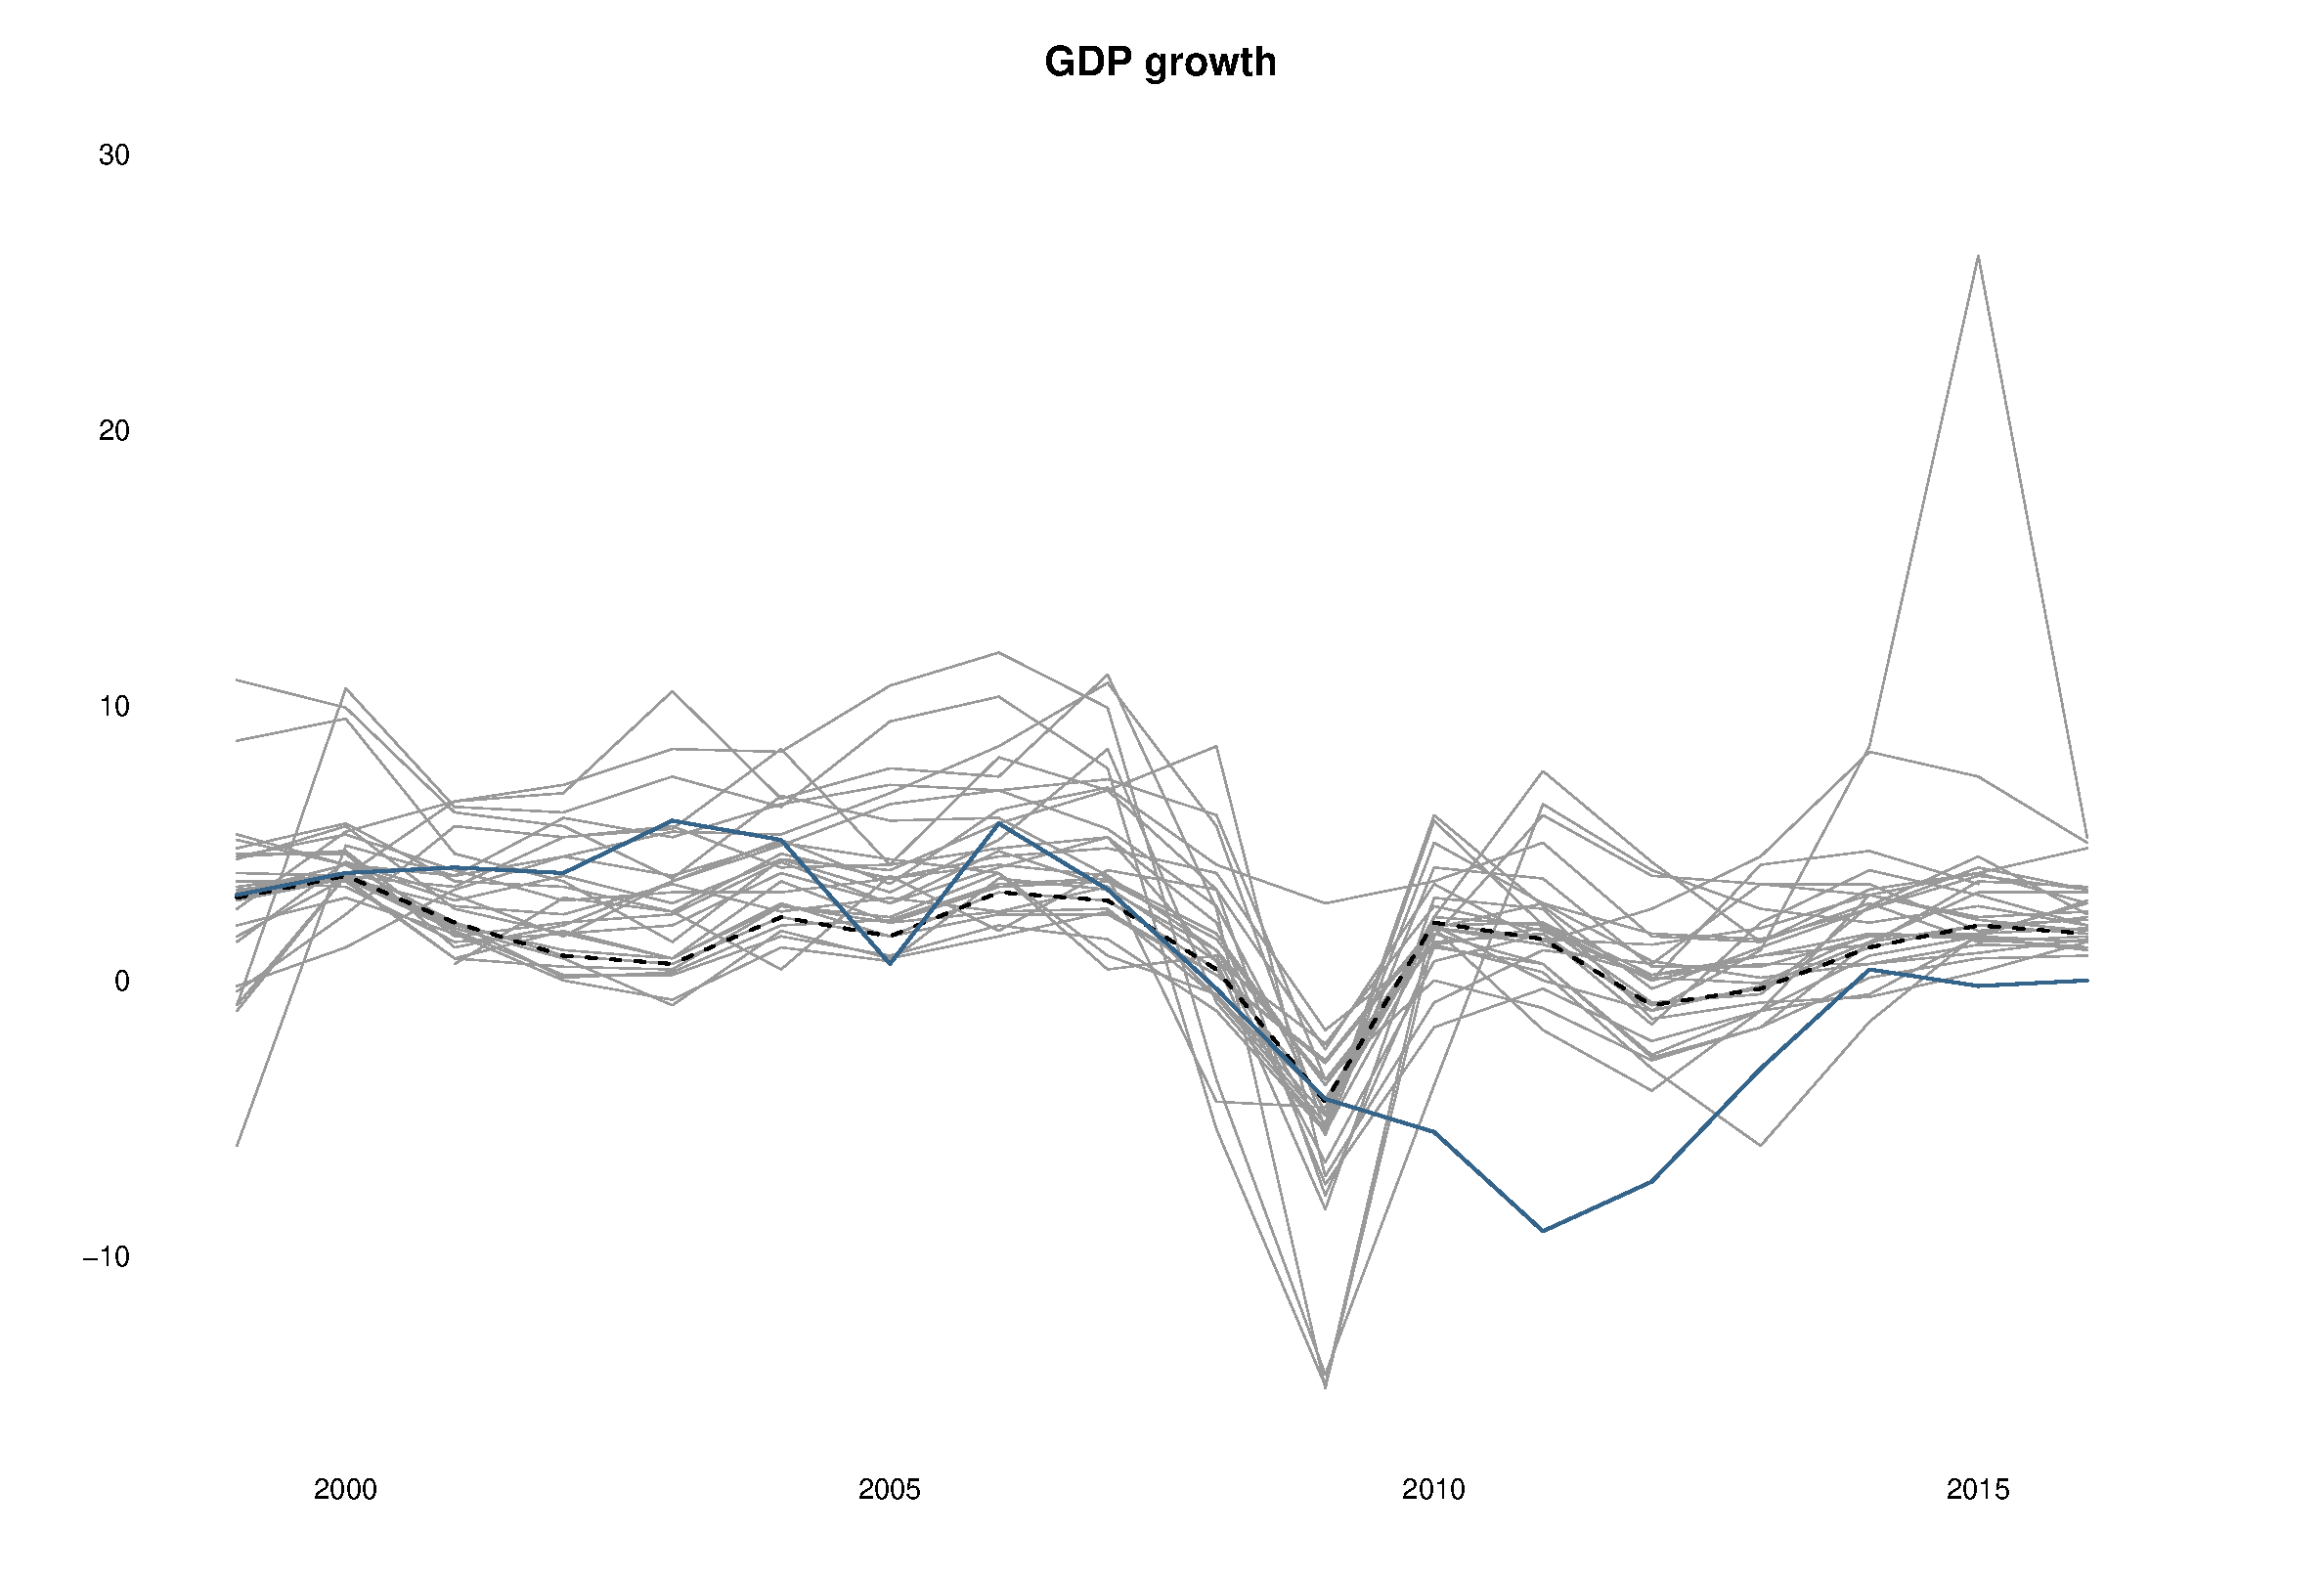
\includegraphics[scale=.3]{gdp_growth.eps}
  \end{figure}
\end{frame}
%--------------------------------------

%--------------------------------------
\begin{frame}
  \begin{figure}
    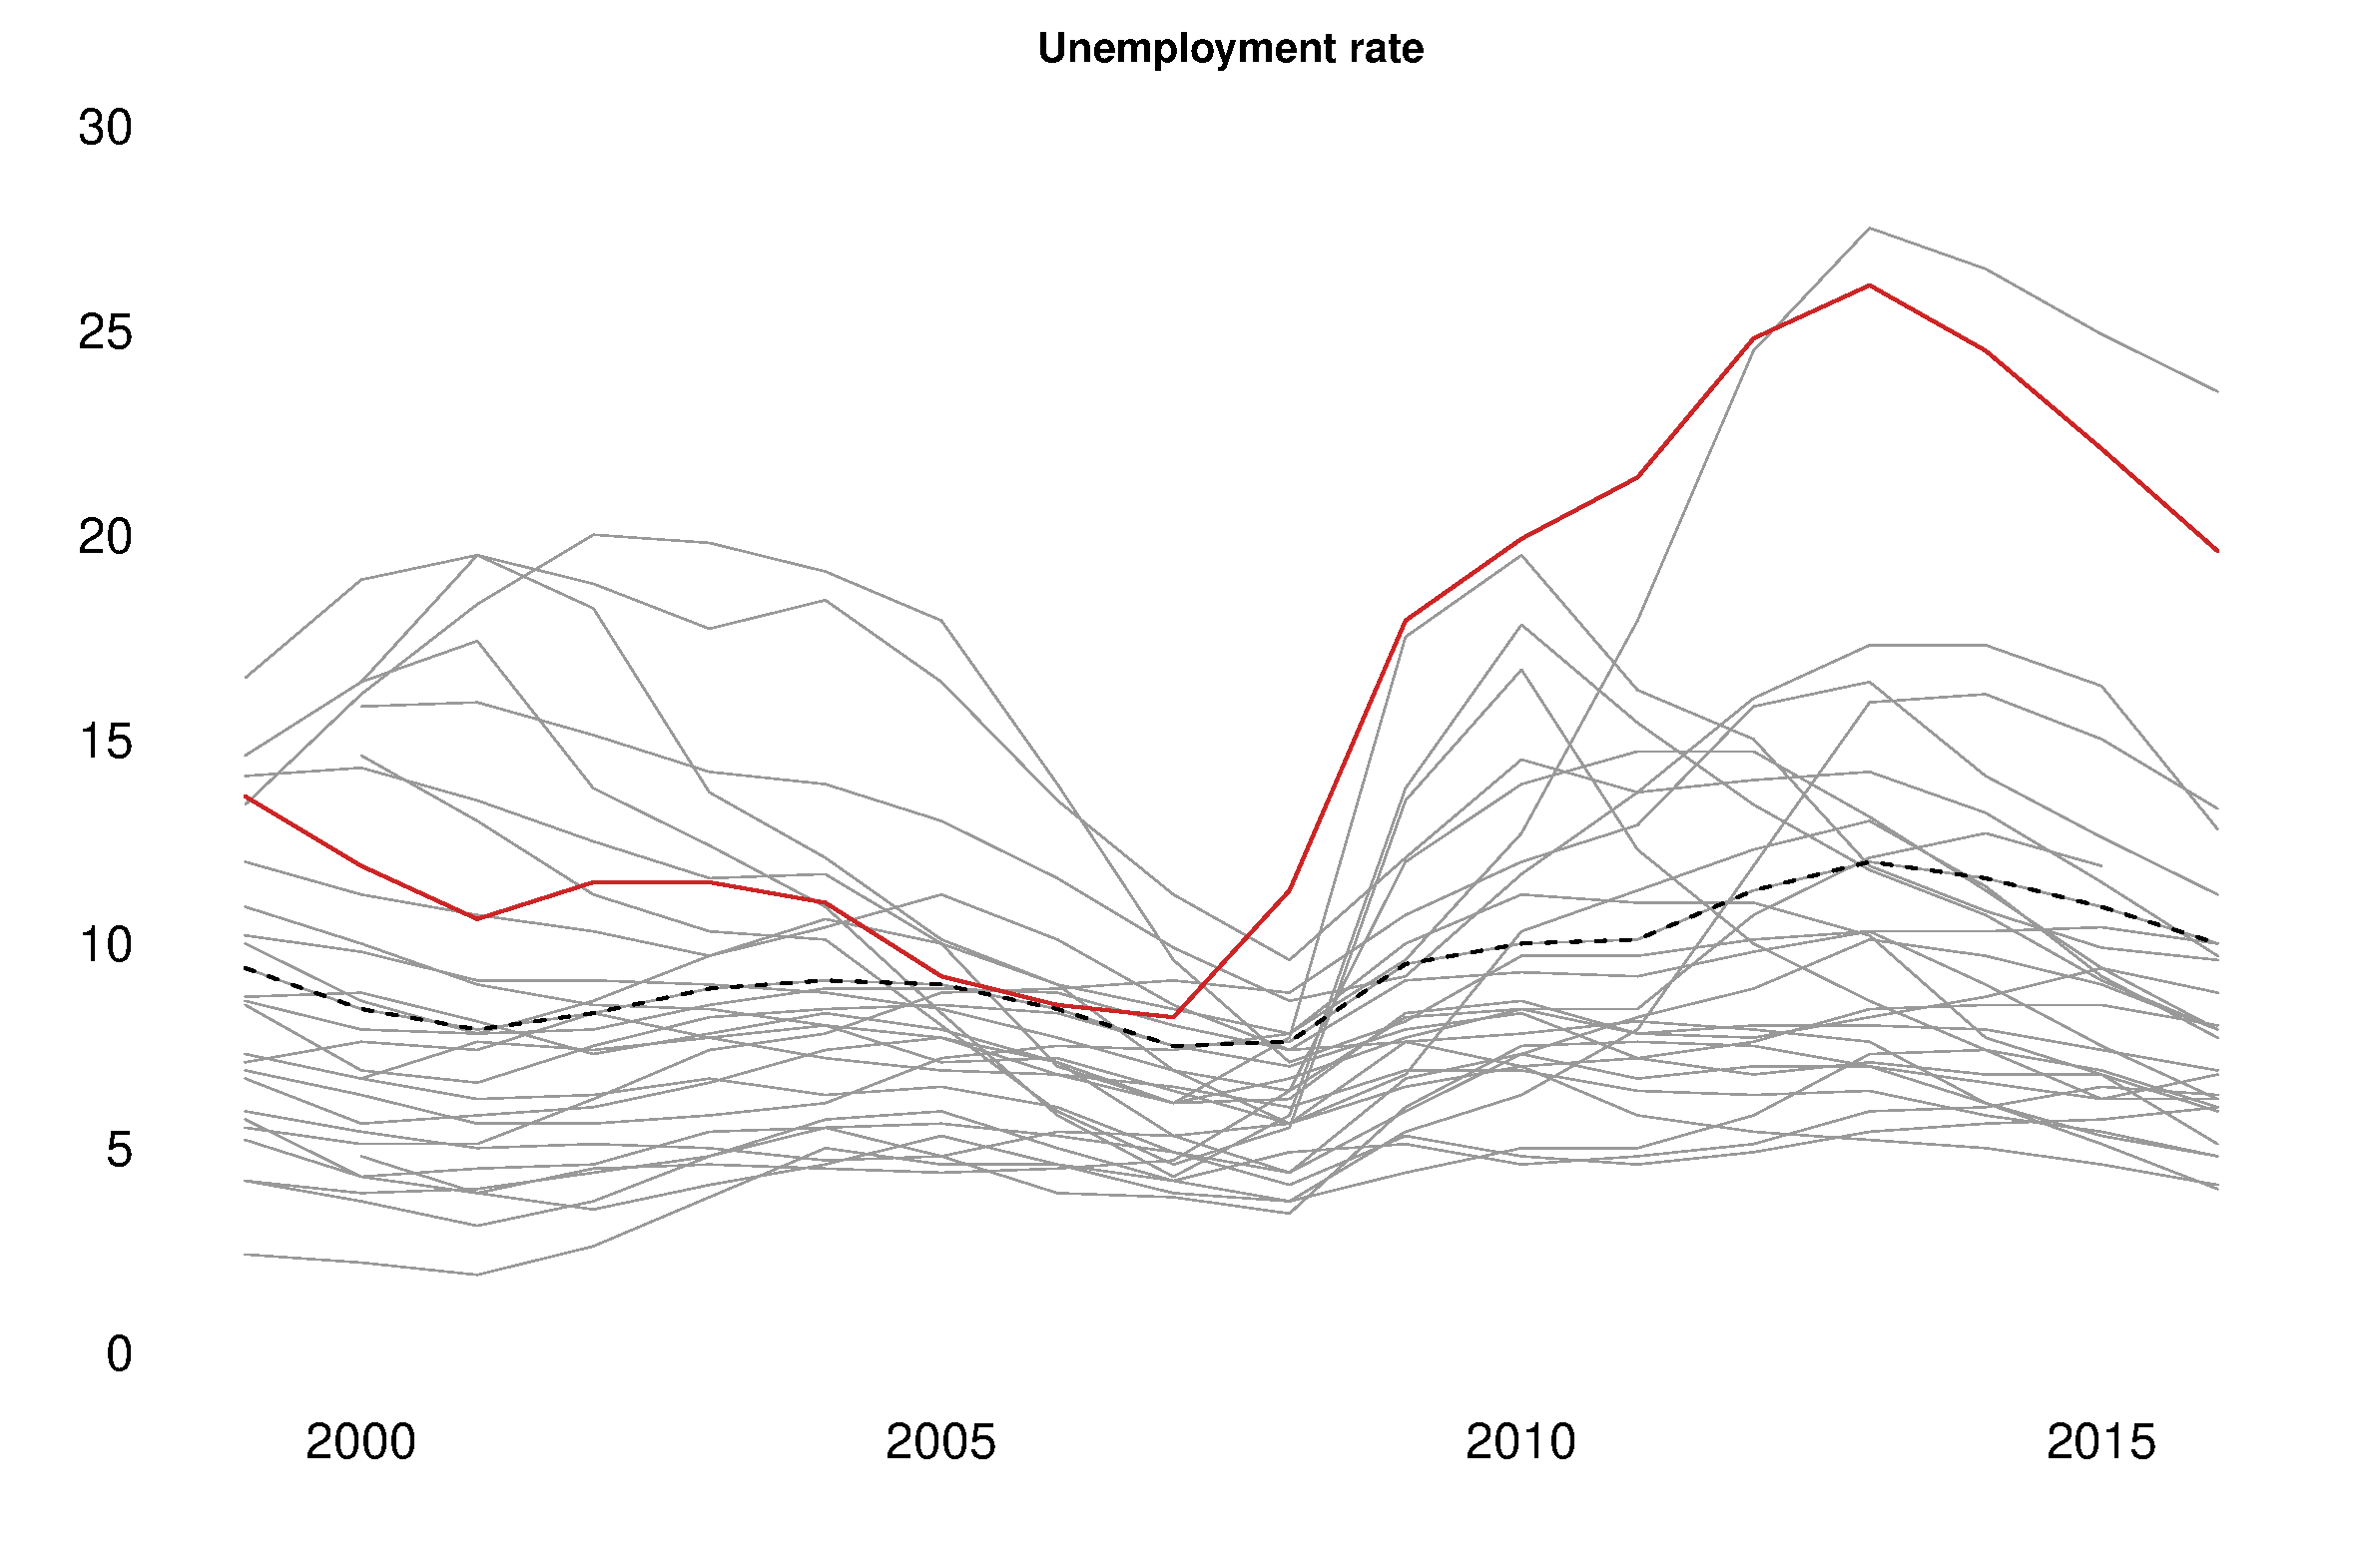
\includegraphics[scale=.3]{unemployment_all.eps}
  \end{figure}
\end{frame}
%--------------------------------------

  
%--------------------------------------
\begin{frame}
  \begin{figure}
    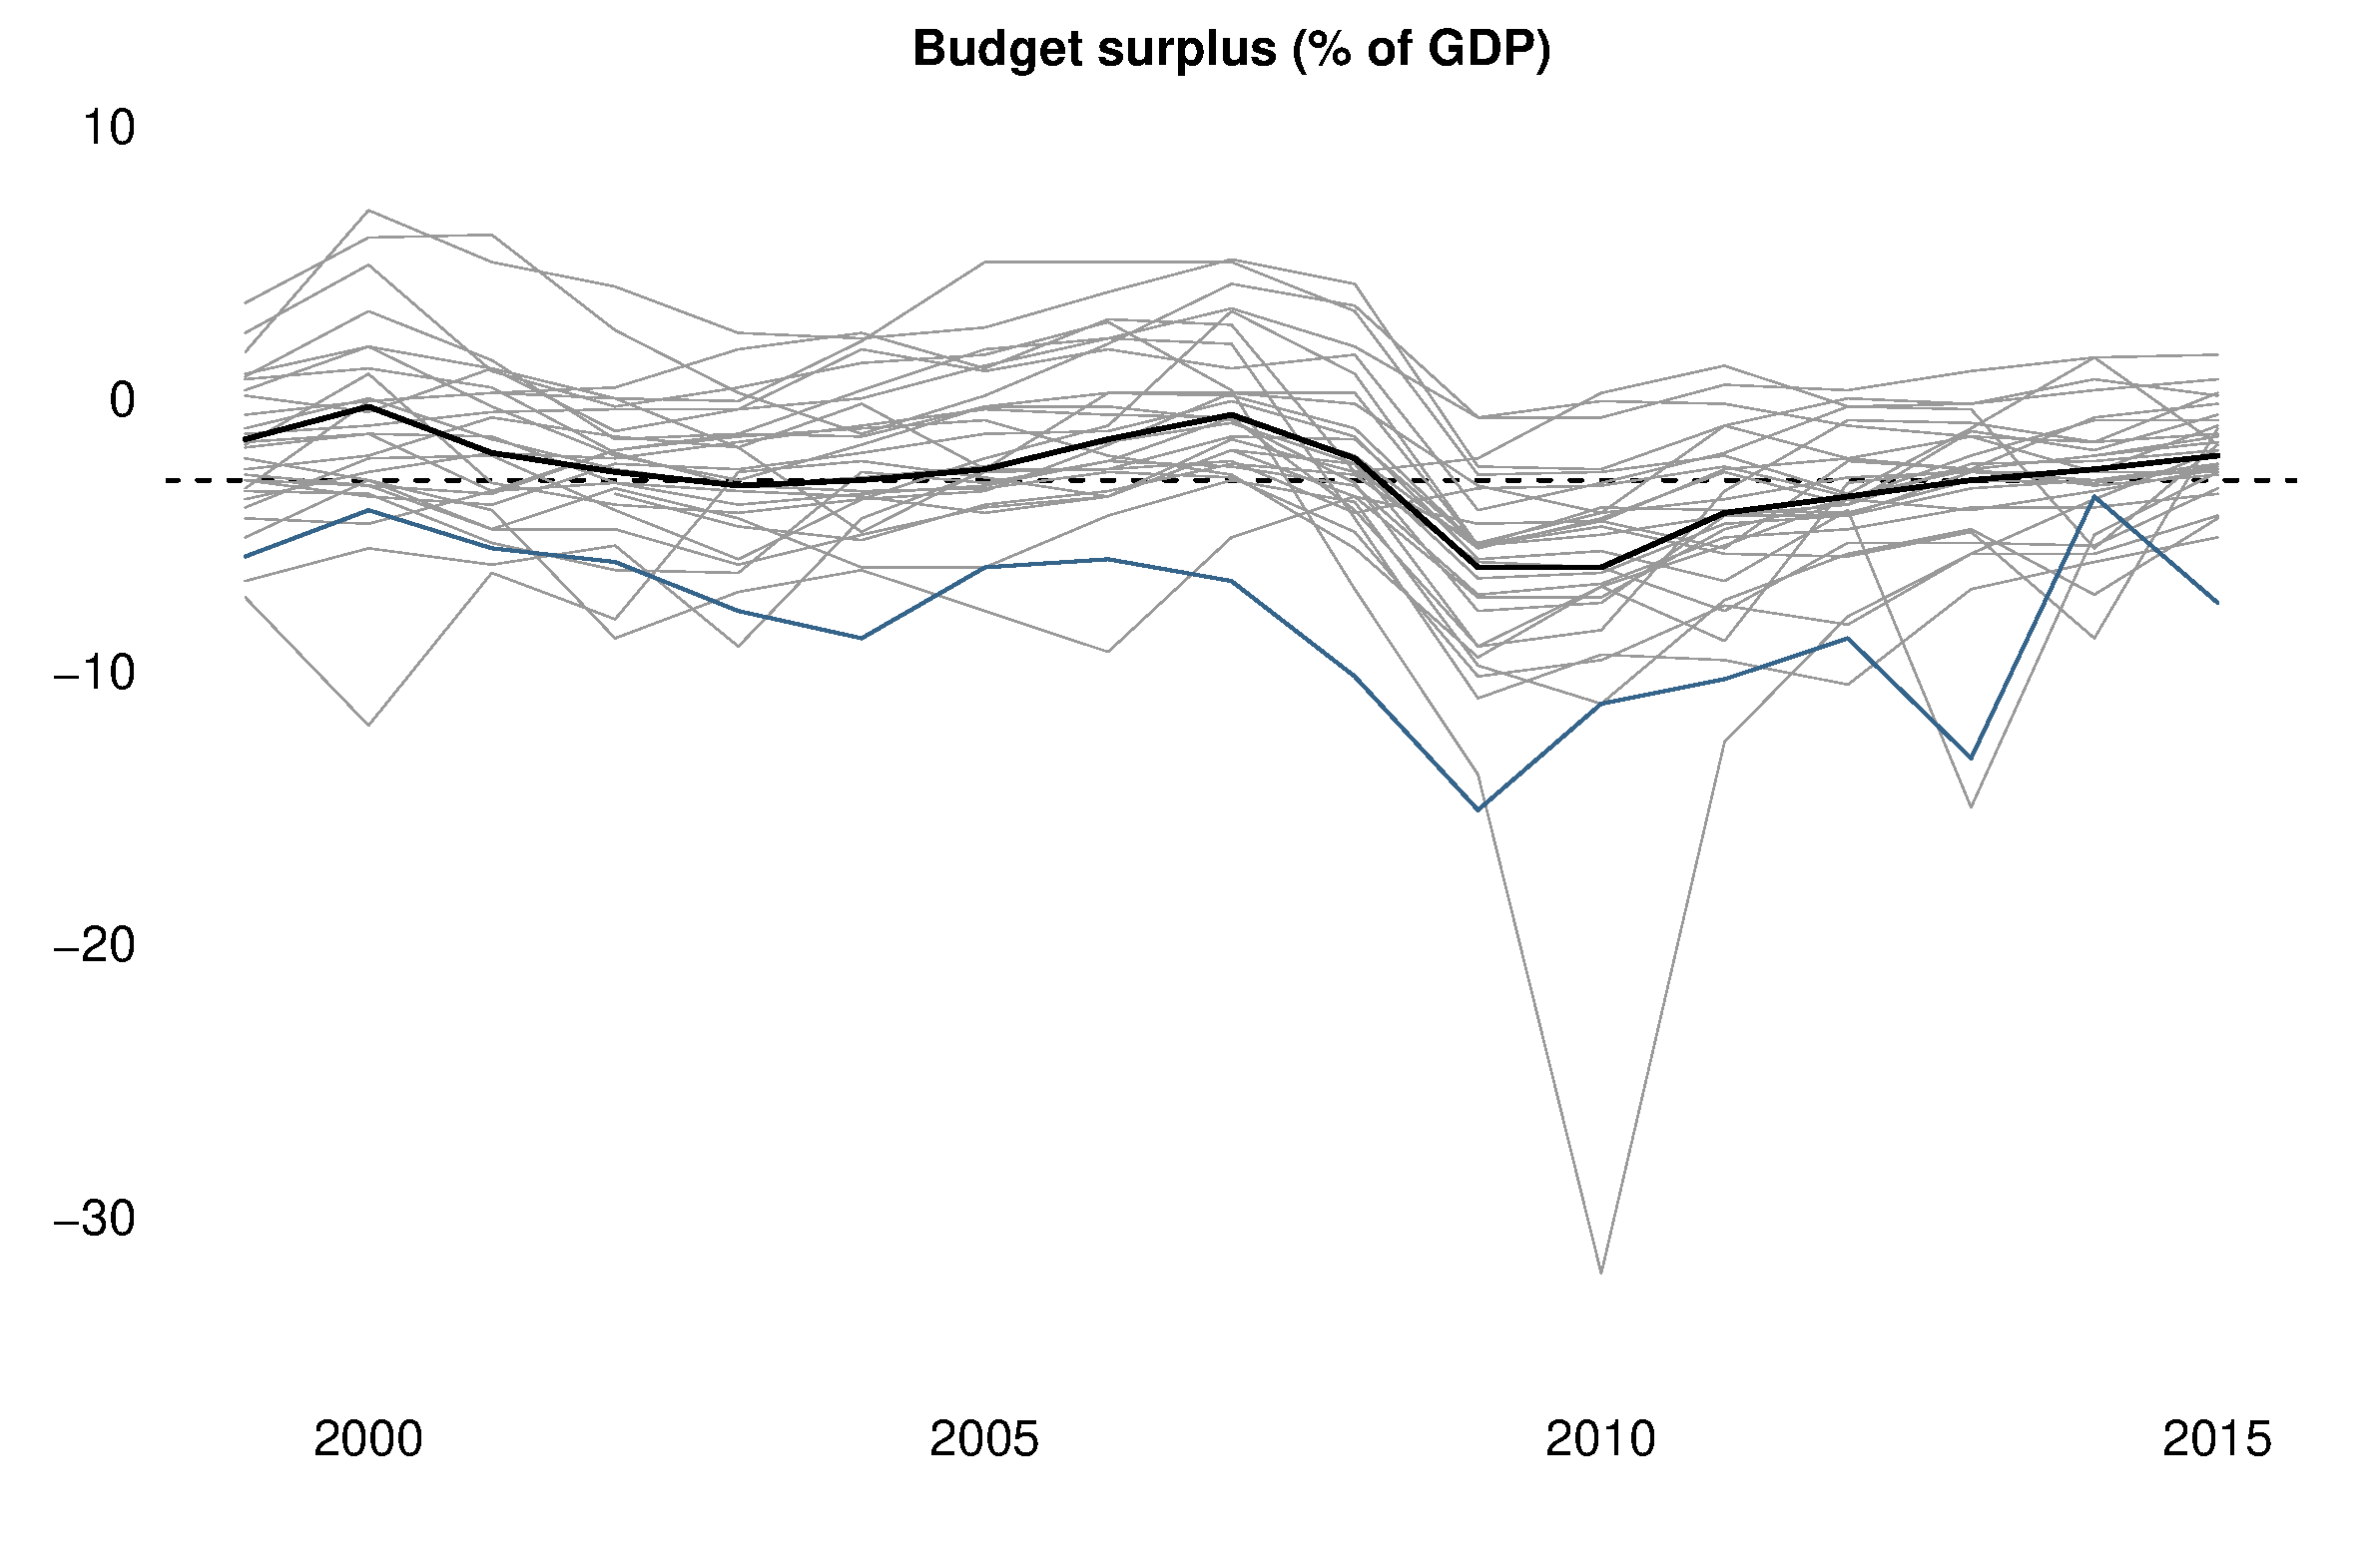
\includegraphics[scale=.3]{budget_surplus.eps}
  \end{figure}
\end{frame}
%--------------------------------------

%--------------------------------------
\begin{frame}
  \begin{figure}
    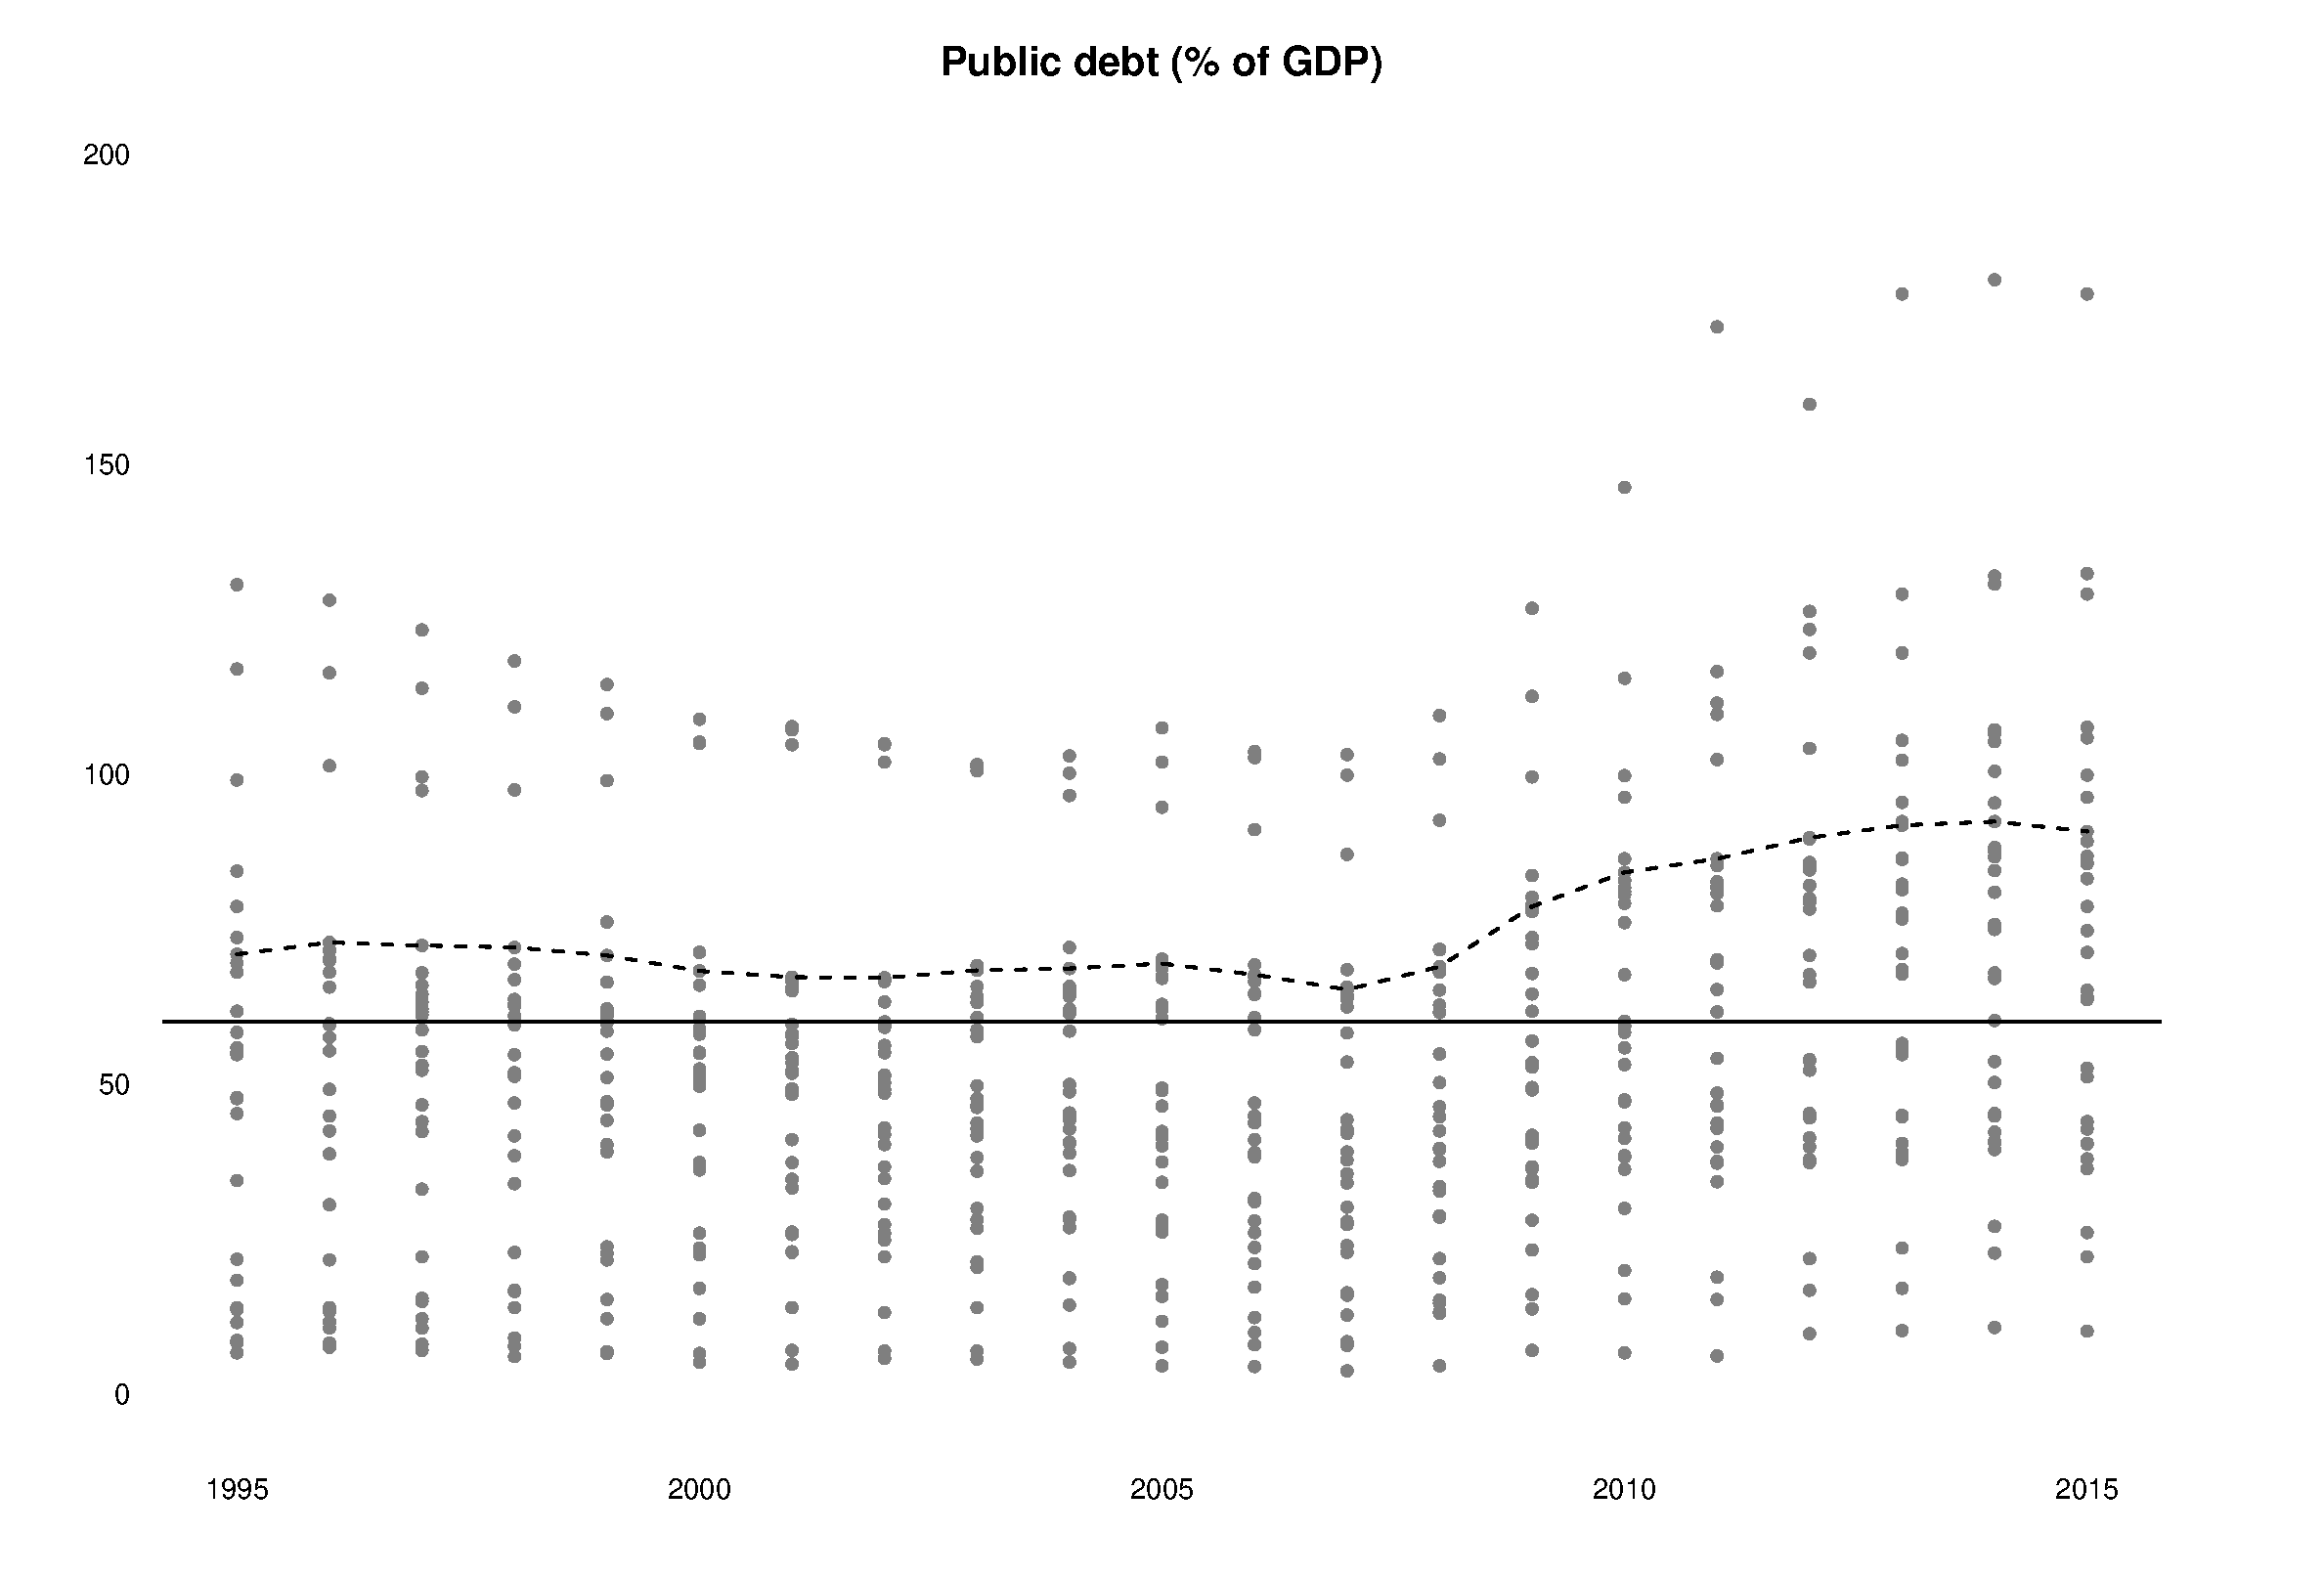
\includegraphics[scale=.3]{public_debt2.eps}
  \end{figure}
\end{frame}
%--------------------------------------

%--------------------------------------
\begin{frame}
  Eurocrisis made two things very clear
  \begin{enumerate}    
    \item Euro design faults
    \item Political inertia
  \end{enumerate}
\end{frame}
%--------------------------------------

%--------------------------------------
\begin{frame}
  \textbf{Euro design faults}\\
  Currency union with common monetary but not fiscal policy
  \begin{itemize}
    \item Complicates matters in terms of crisis response
    \item Even with EU coordination on fiscal policy (differences in debt levels)
  \end{itemize}  
\end{frame}
%--------------------------------------

%--------------------------------------
\begin{frame}
\textbf{Lisbon treaty} article 125
\scalebox{.7}{
\begin{quote}
  1. The Union shall not be liable for or assume the commitments of central governments, regional, local or other public authorities, other bodies governed by public law, or public undertakings of any Member State, without prejudice to mutual financial guarantees for the joint execution of a specific project. A Member State shall not be liable for or assume the commitments of central governments, regional, local or other public authorities, other bodies governed by public law, or public undertakings of another Member State, without prejudice to mutual financial guarantees for the joint execution of a specific project.

  2. The Council, on a proposal from the Commission and after consulting the European Parliament, may, as required, specify definitions for the application of the prohibitions referred to in Articles 123 and 124 and in this Article.
\end{quote}}
\end{frame}
%--------------------------------------

%--------------------------------------
\begin{frame}
  \textbf{Lisbon treaty} article 122
  \scalebox{.7}{
  \begin{quote}
    1. Without prejudice to any other procedures provided for in the Treaties, the Council, on a proposal from the Commission, may decide, in a spirit of solidarity between Member States, upon the measures appropriate to the economic situation, in particular if severe difficulties arise in the supply of certain products, notably in the area of energy.

    2. Where a Member State is in difficulties or is seriously threatened with severe difficulties caused by natural disasters or exceptional occurrences beyond its control, the Council, on a proposal from the Commission, may grant, under certain conditions, Union financial assistance to the Member State concerned. The President of the Council shall inform the European Parliament of the decision taken.
  \end{quote}}
\end{frame}
%--------------------------------------


%--------------------------------------
\begin{frame}
  \begin{figure}
    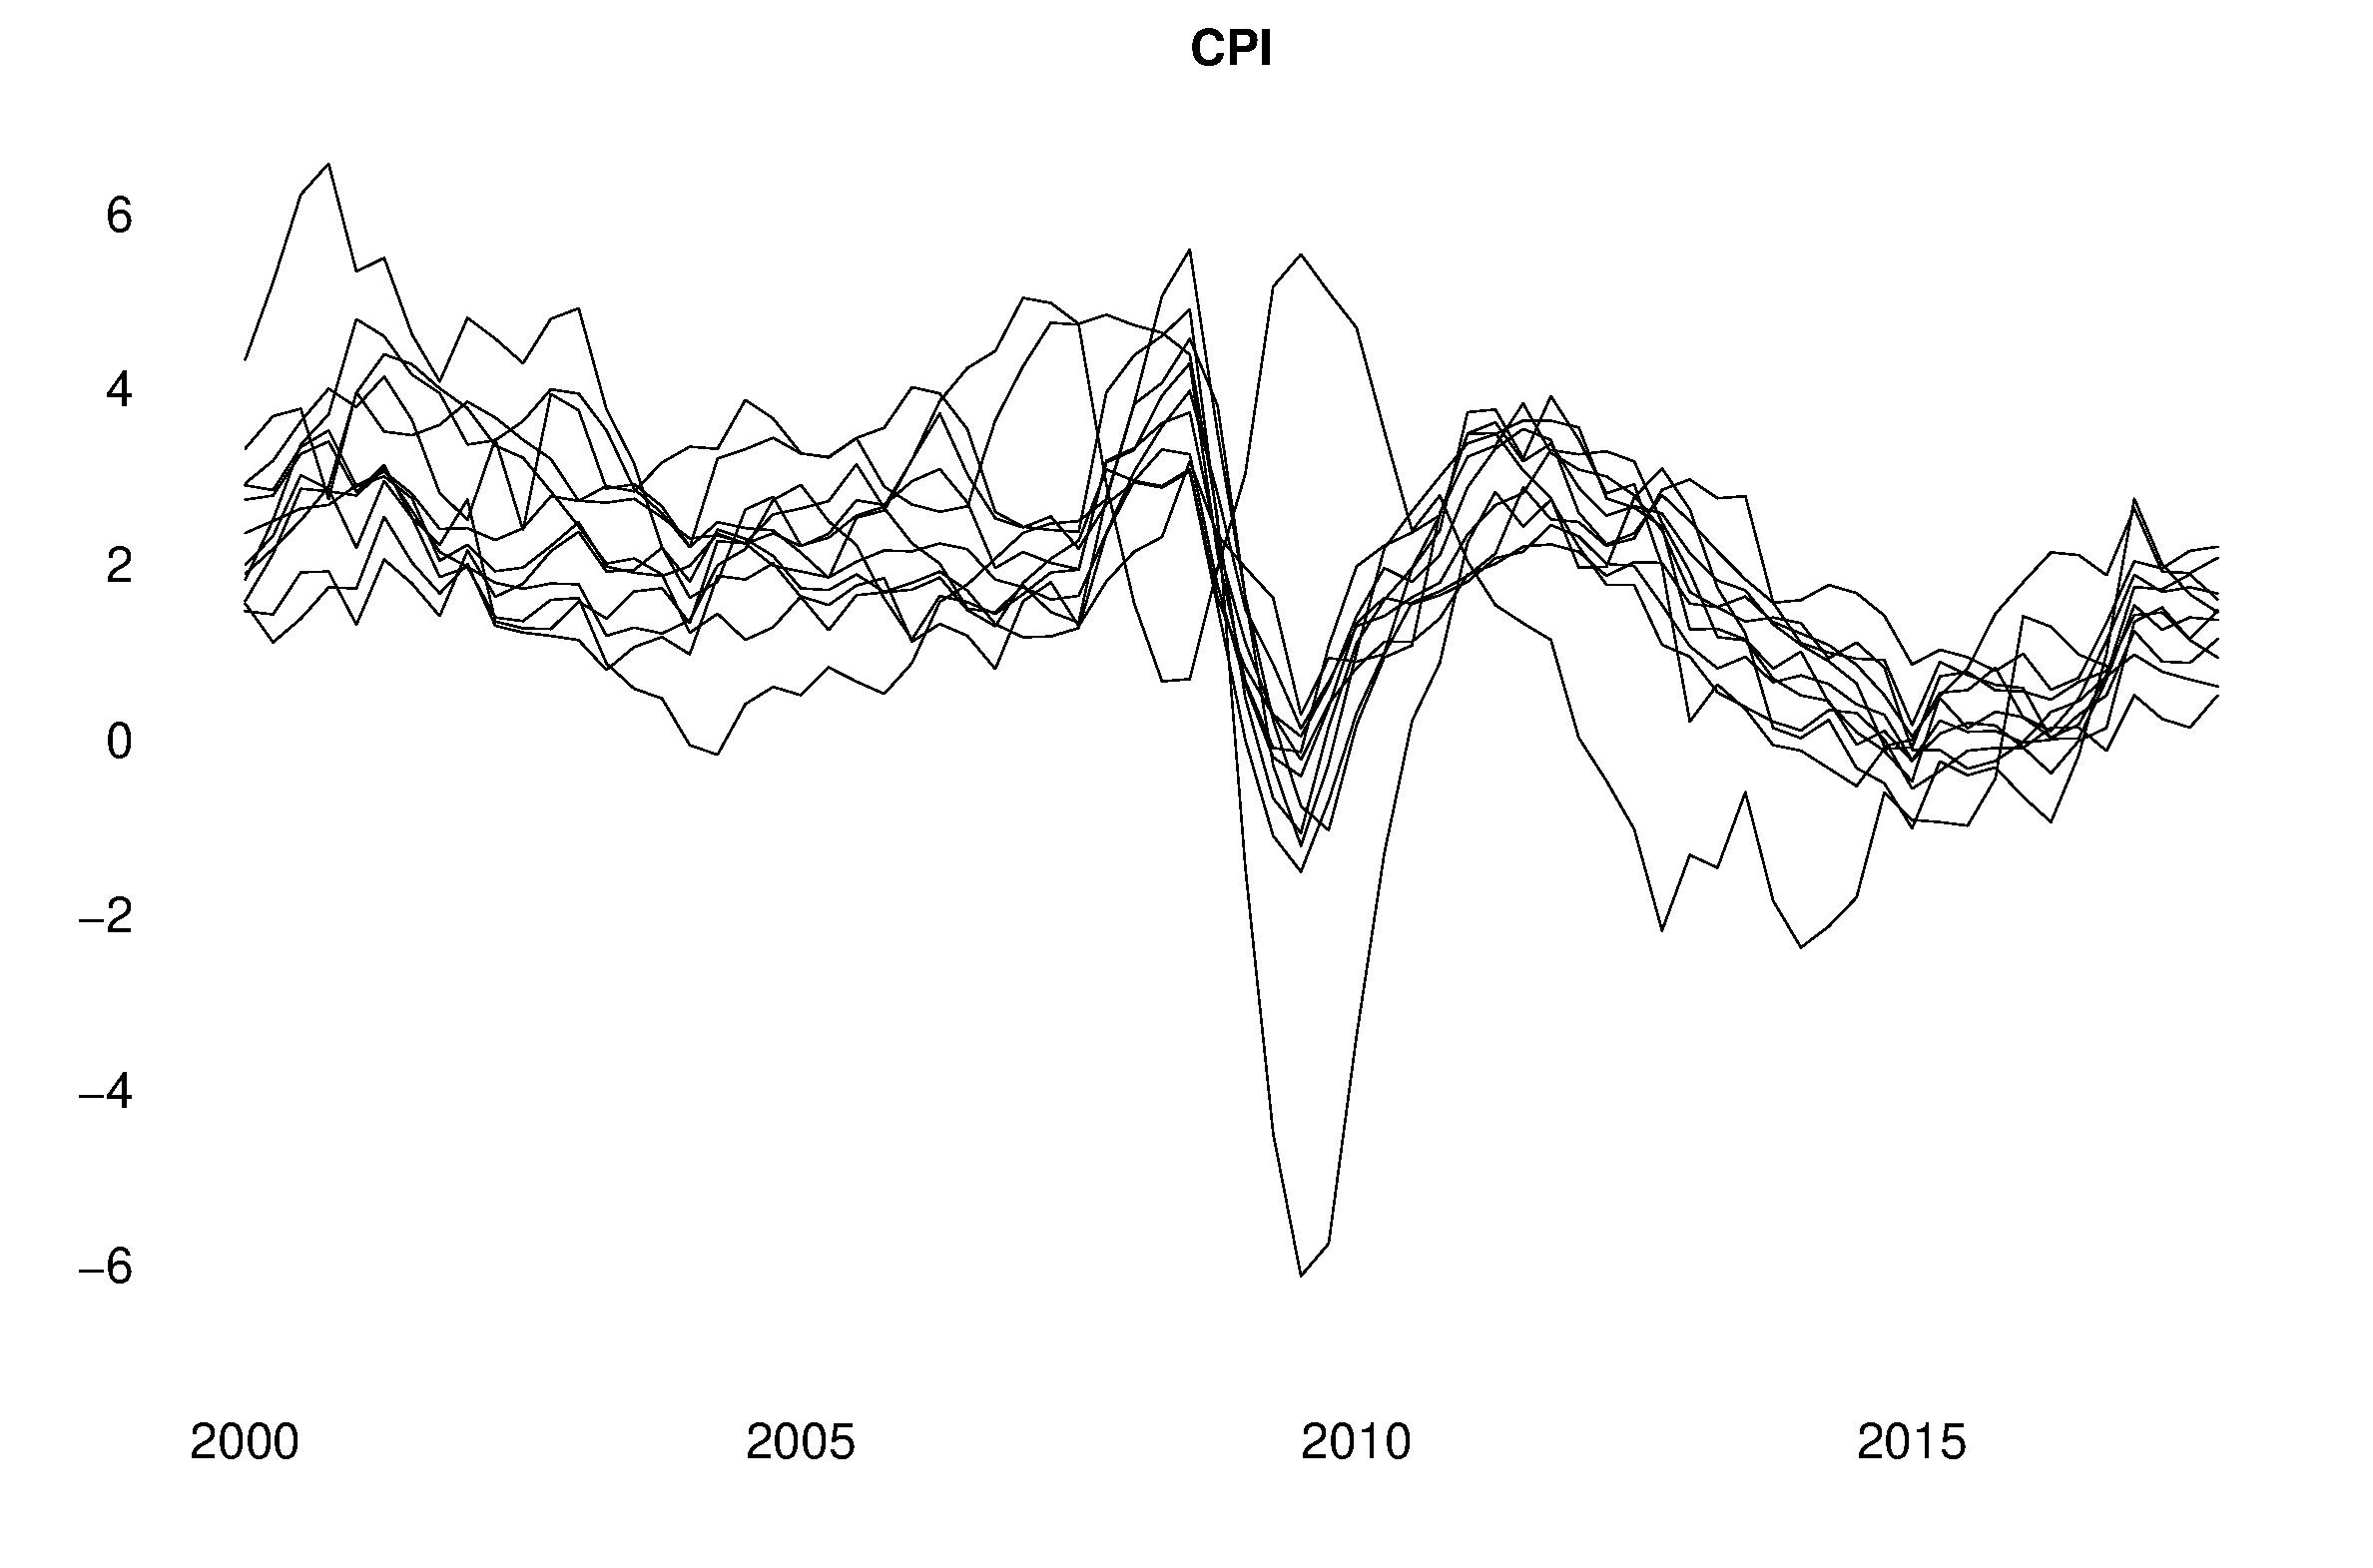
\includegraphics[scale=.3]{inflation_eurozone2.eps}
  \end{figure}
\end{frame}
%--------------------------------------

%--------------------------------------
\begin{frame}
  \textbf{Inflation differences}\\
  OCA theory emphasises risk of 
  \begin{enumerate}
    \item Asymmetric shocks
    \item Symmetric shock with asymmetric effect (e.g. Great recession)
  \end{enumerate}
  \medskip
  Main issue: inflation rates
  \begin{itemize}
    \item e.g. Greece/Italy persistent higher inflation rates compared to Germany
  \end{itemize}
  \medskip
  Countries cannot devalue their currency to regain competitiveness 
  \begin{itemize}
    \item ECB sets monetary policy
    \item Appreciation of real exchange rate
  \end{itemize}  
\end{frame}
%--------------------------------------

%--------------------------------------
\begin{frame}
  Consider one good which is sold in two countries
  \begin{enumerate}
    \item Italy
    \item Germany
  \end{enumerate}
  Price in Italy is: $p$\\
  Price in Germany is: $p^*$\\
  \medskip  
  Pre-euro: compare prices using exchange rate $E$.\\
  Real exchange rate given by
  \begin{align}
    \frac{Ep}{p^*}
  \end{align}  
\end{frame}
%--------------------------------------

%--------------------------------------
\begin{frame}  
  With  euro $E$ is fixed; inflation causes increase in 
  \begin{align}
    \frac{p}{p^*}
  \end{align}
  \medskip
  Appreciation in 
  \begin{align}
    \frac{Ep}{p^*}
  \end{align}
  \medskip
  Result: loss in competitiveness. 
\end{frame}
%--------------------------------------

%--------------------------------------
\begin{frame}
 Various explanations for diverging inflation rates
 \begin{itemize}
   \item Balassa-Samuelson effect
   \item ECU fixed at wrong rates
 \end{itemize}
\end{frame}
%--------------------------------------

%--------------------------------------
\begin{frame}
  Various explanations for diverging inflation rates (cont.)
\begin{itemize}  
  \item Autonomous wage and price setting
  \begin{itemize}
    \item Wage increases caused by factors other than labour productivity decreases competitiveness
    \item e.g. raising minimum wage, bargaining by sectors that don't face much competition such as civil servants, administered prices in transport and energy
  \end{itemize}
  \item Policy mistakes
  \begin{itemize}
    \item e.g. government increases prices/wages through expansionary fiscal policies
  \end{itemize}  
  \item Different preferences
  \begin{itemize}
    \item Inflation tax/seigniorage preferred when country is poor at collecting taxes
    \item Different consumption baskets can cause different inflations across countries with same monetary policy
  \end{itemize}
\end{itemize}
\end{frame}
%--------------------------------------

%--------------------------------------
\begin{frame}
  \textbf{Political inertia}\\
  Negotiations led to kicking the can further down the road
  \begin{itemize}
    \item Bail outs granted; no structural reforms implemented
    \item Recall; no fiscal transfers
  \end{itemize}
  \medskip
  Symmetric shock led to asymmetric effects
  \begin{itemize}
    \item Differences across countries on desired approach to deal with problem
  \end{itemize}
\end{frame}
%--------------------------------------

%--------------------------------------
\begin{frame}
  Juncker's populism
  \begin{quote}
    Financial markets are clearly wrong if they believe they can break Greece into little bits.
  \end{quote}
  \begin{quote}
    We have to strengthen the primacy of politics. We have to be able to stop financial markets. We have instruments of torture in the basement. We will display them if it becomes necessary.
  \end{quote}
\end{frame}
%--------------------------------------

%--------------------------------------
\begin{frame}
  Number of factors amplified Great Recession in Europe
  \begin{enumerate}
    \item Level of public debt
    \item Trade imbalances
    \item Financial integration
  \end{enumerate}
\end{frame}
%--------------------------------------

%--------------------------------------
\begin{frame}
  \begin{figure}
    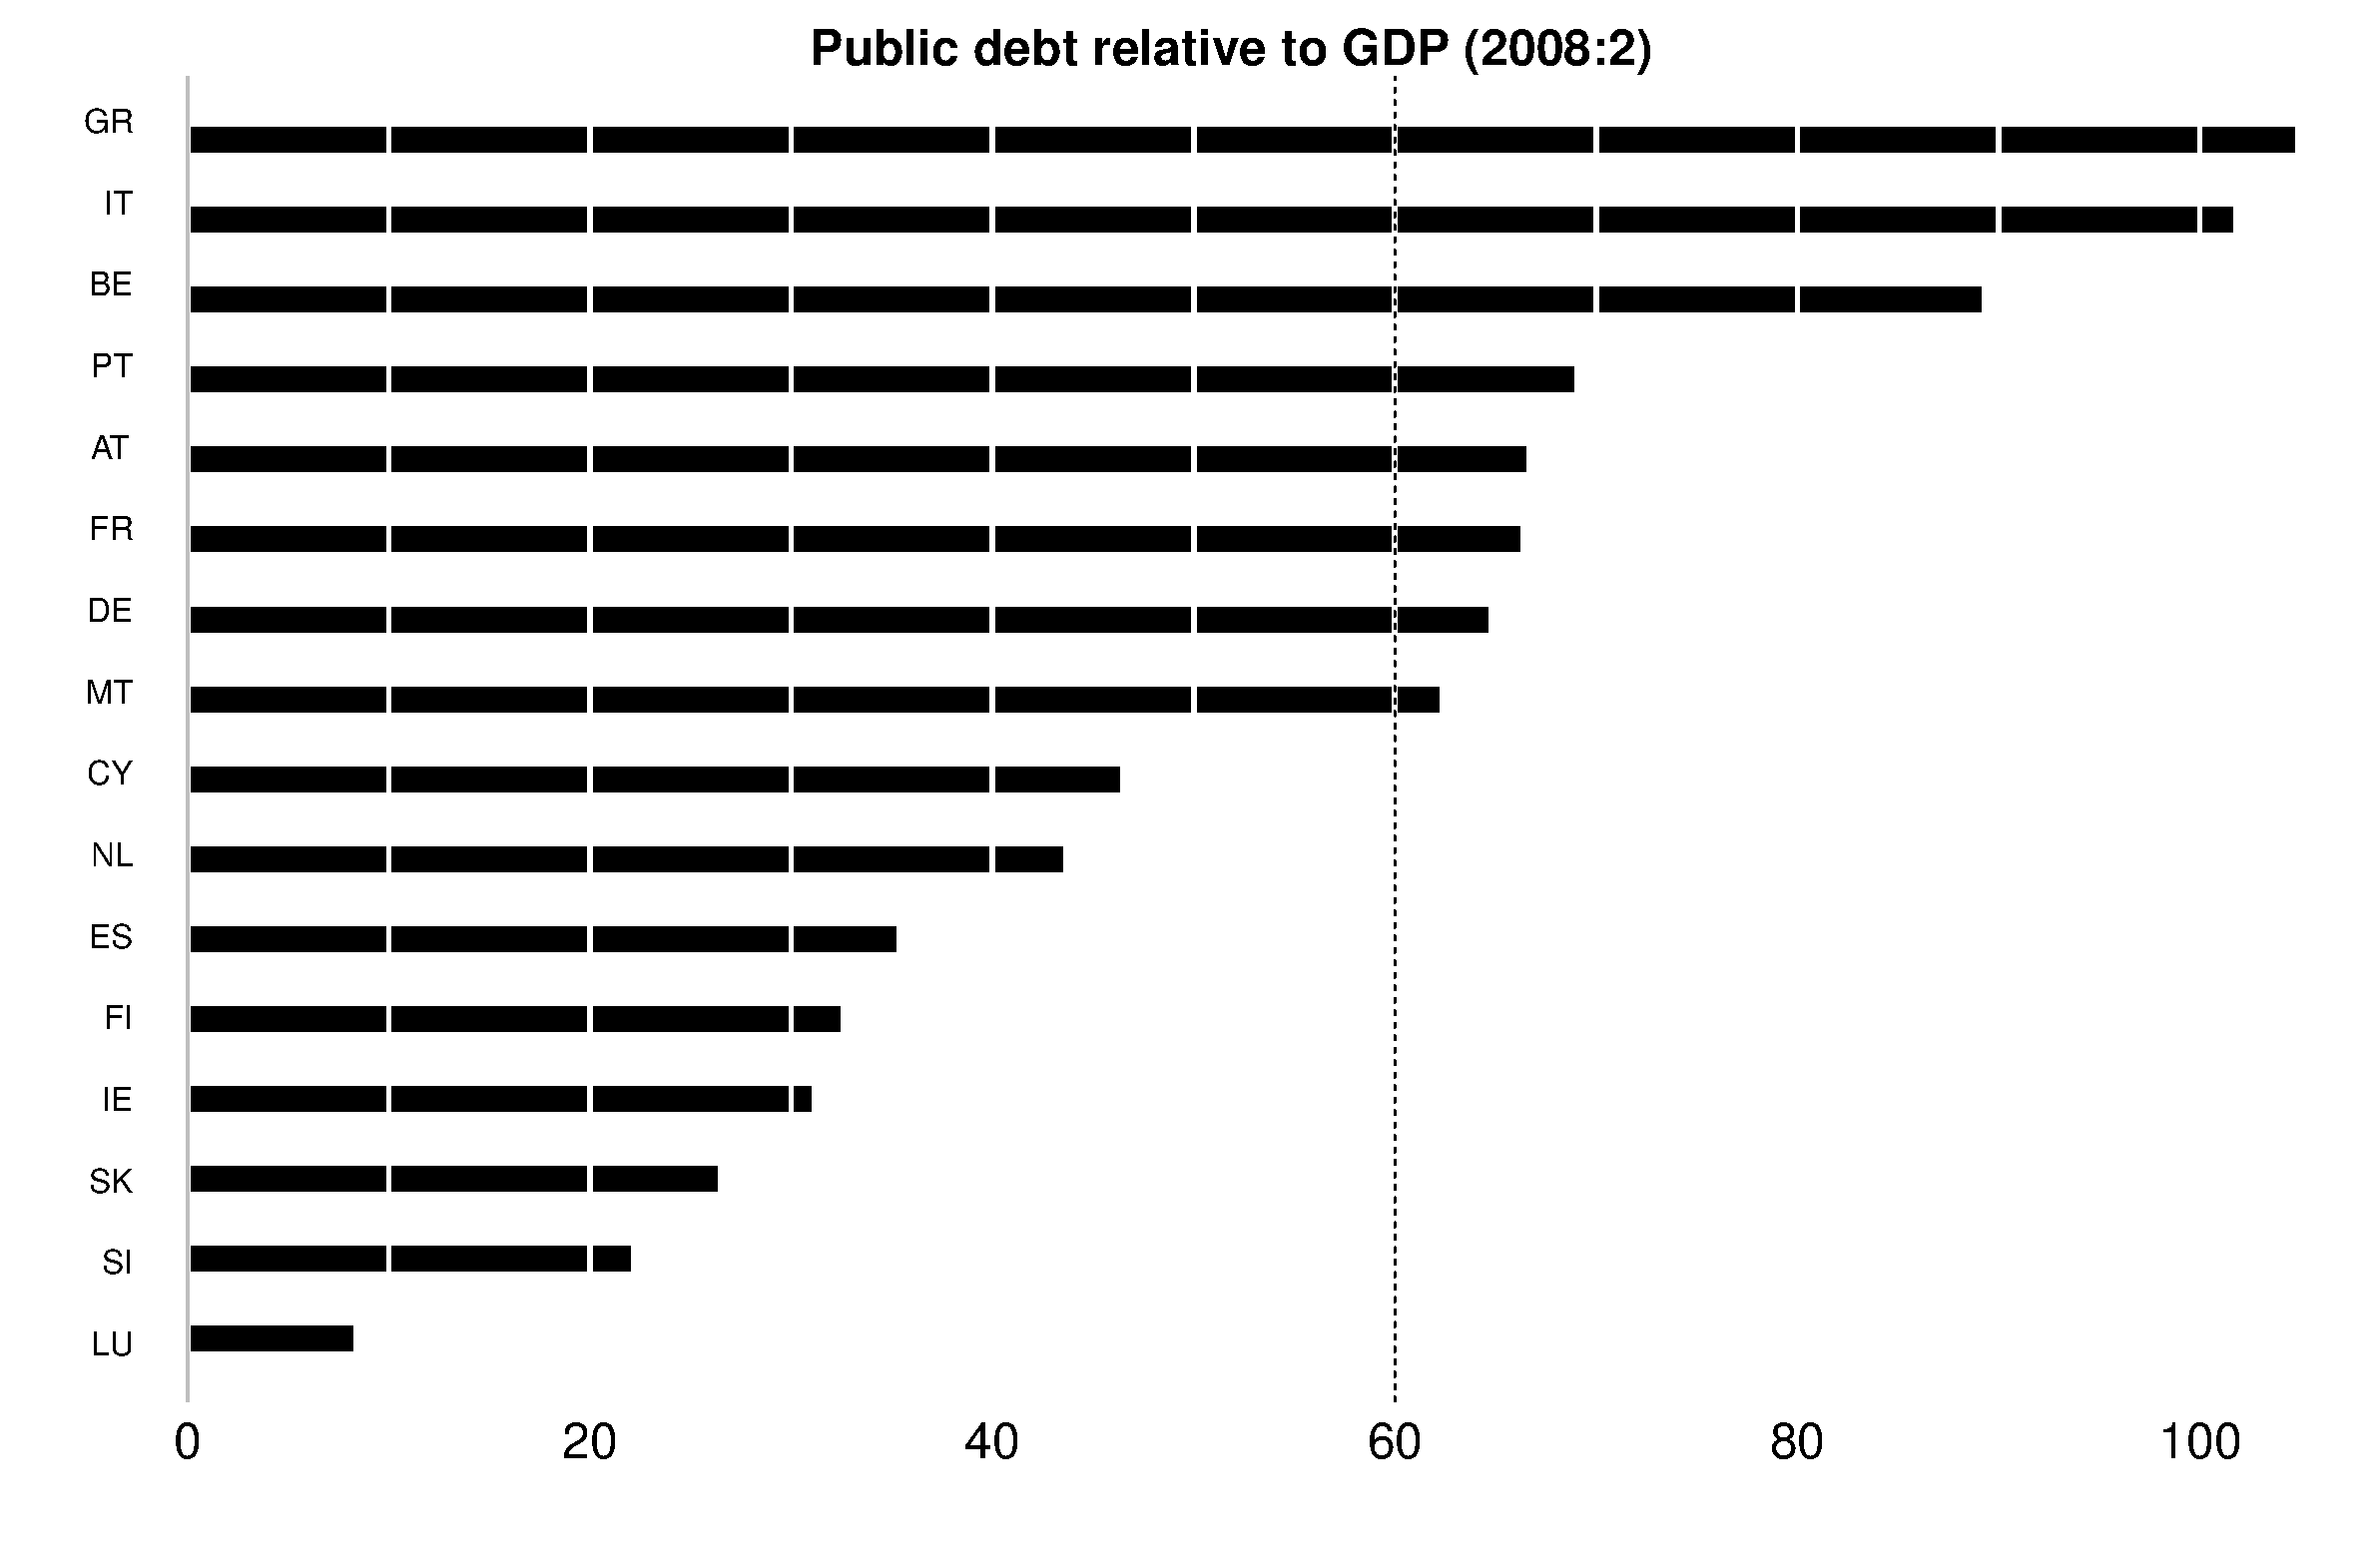
\includegraphics[scale=.3]{public_debt_eurozone2.eps}
  \end{figure}
\end{frame}
%--------------------------------------

%--------------------------------------
\begin{frame}
  \begin{figure}
    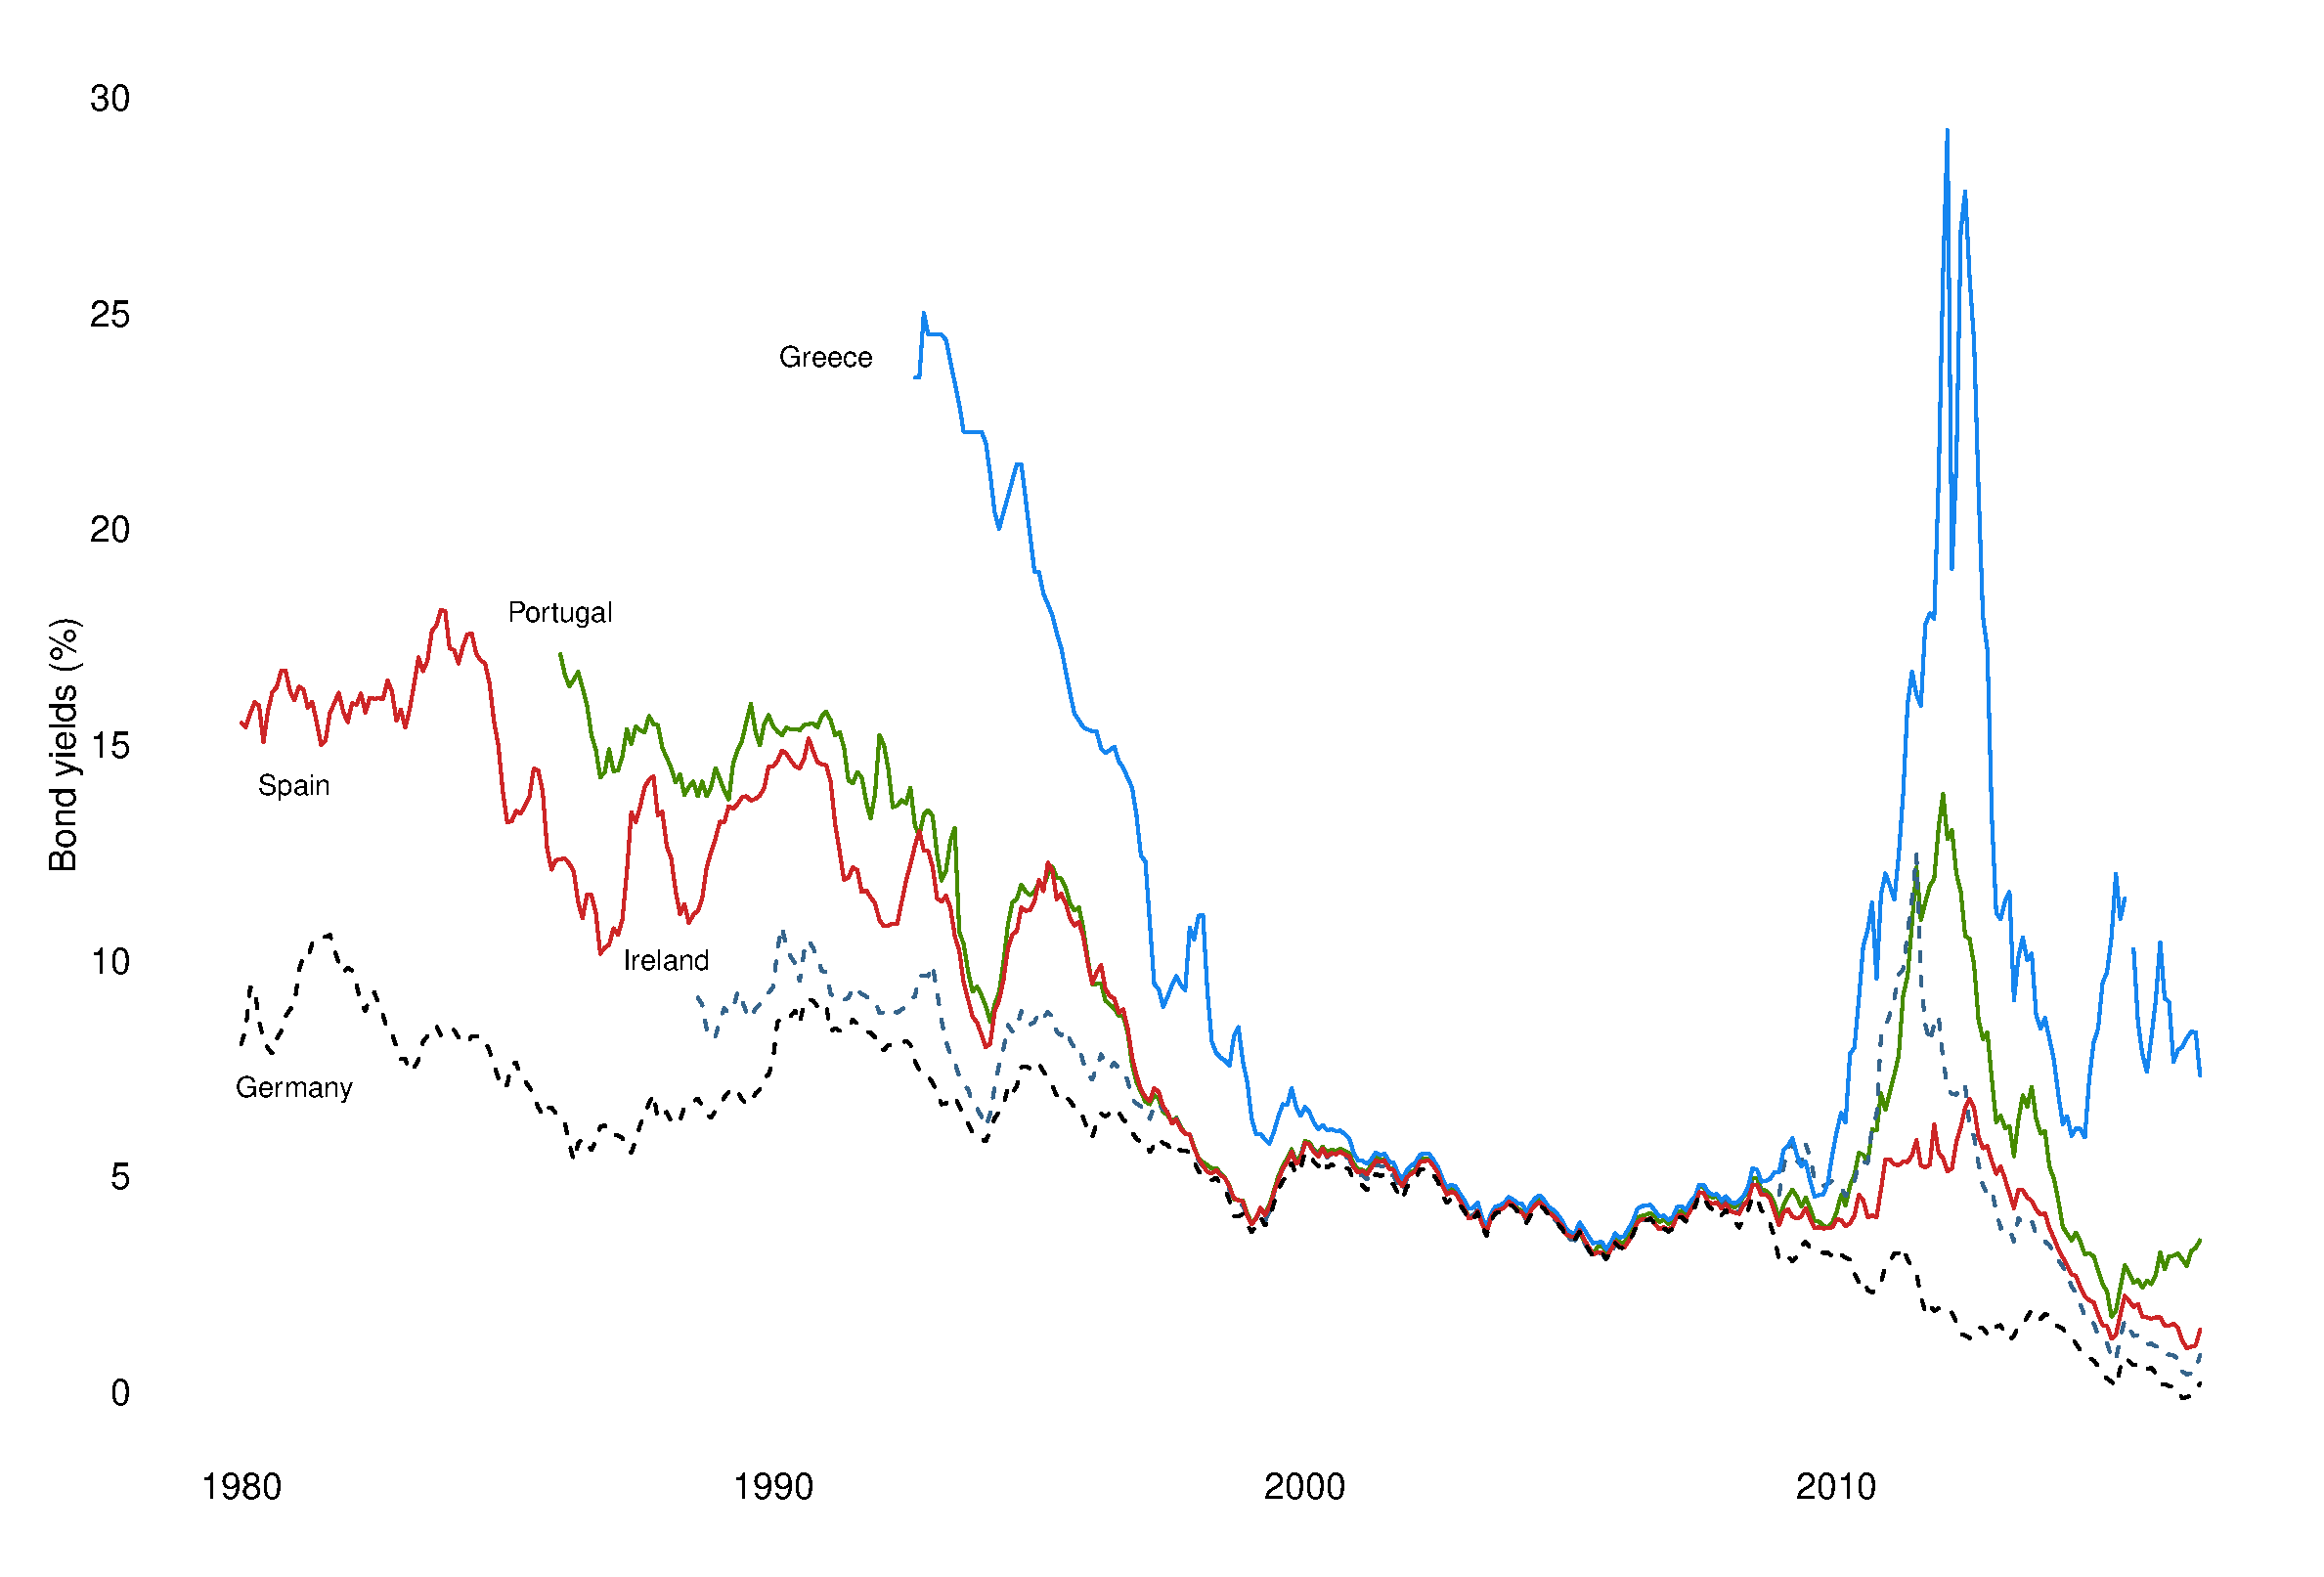
\includegraphics[scale=.3]{bonds.eps}
  \end{figure}
\end{frame}
%--------------------------------------

%--------------------------------------
\begin{frame}
  \begin{figure}
    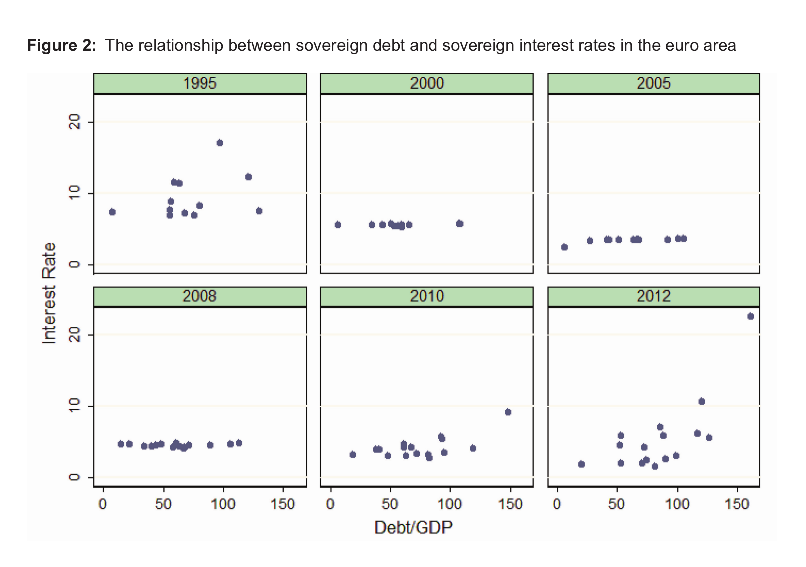
\includegraphics[scale=.9]{whelan.eps}
  \end{figure}
\end{frame}
%--------------------------------------


%--------------------------------------
\begin{frame}
  \begin{figure}
    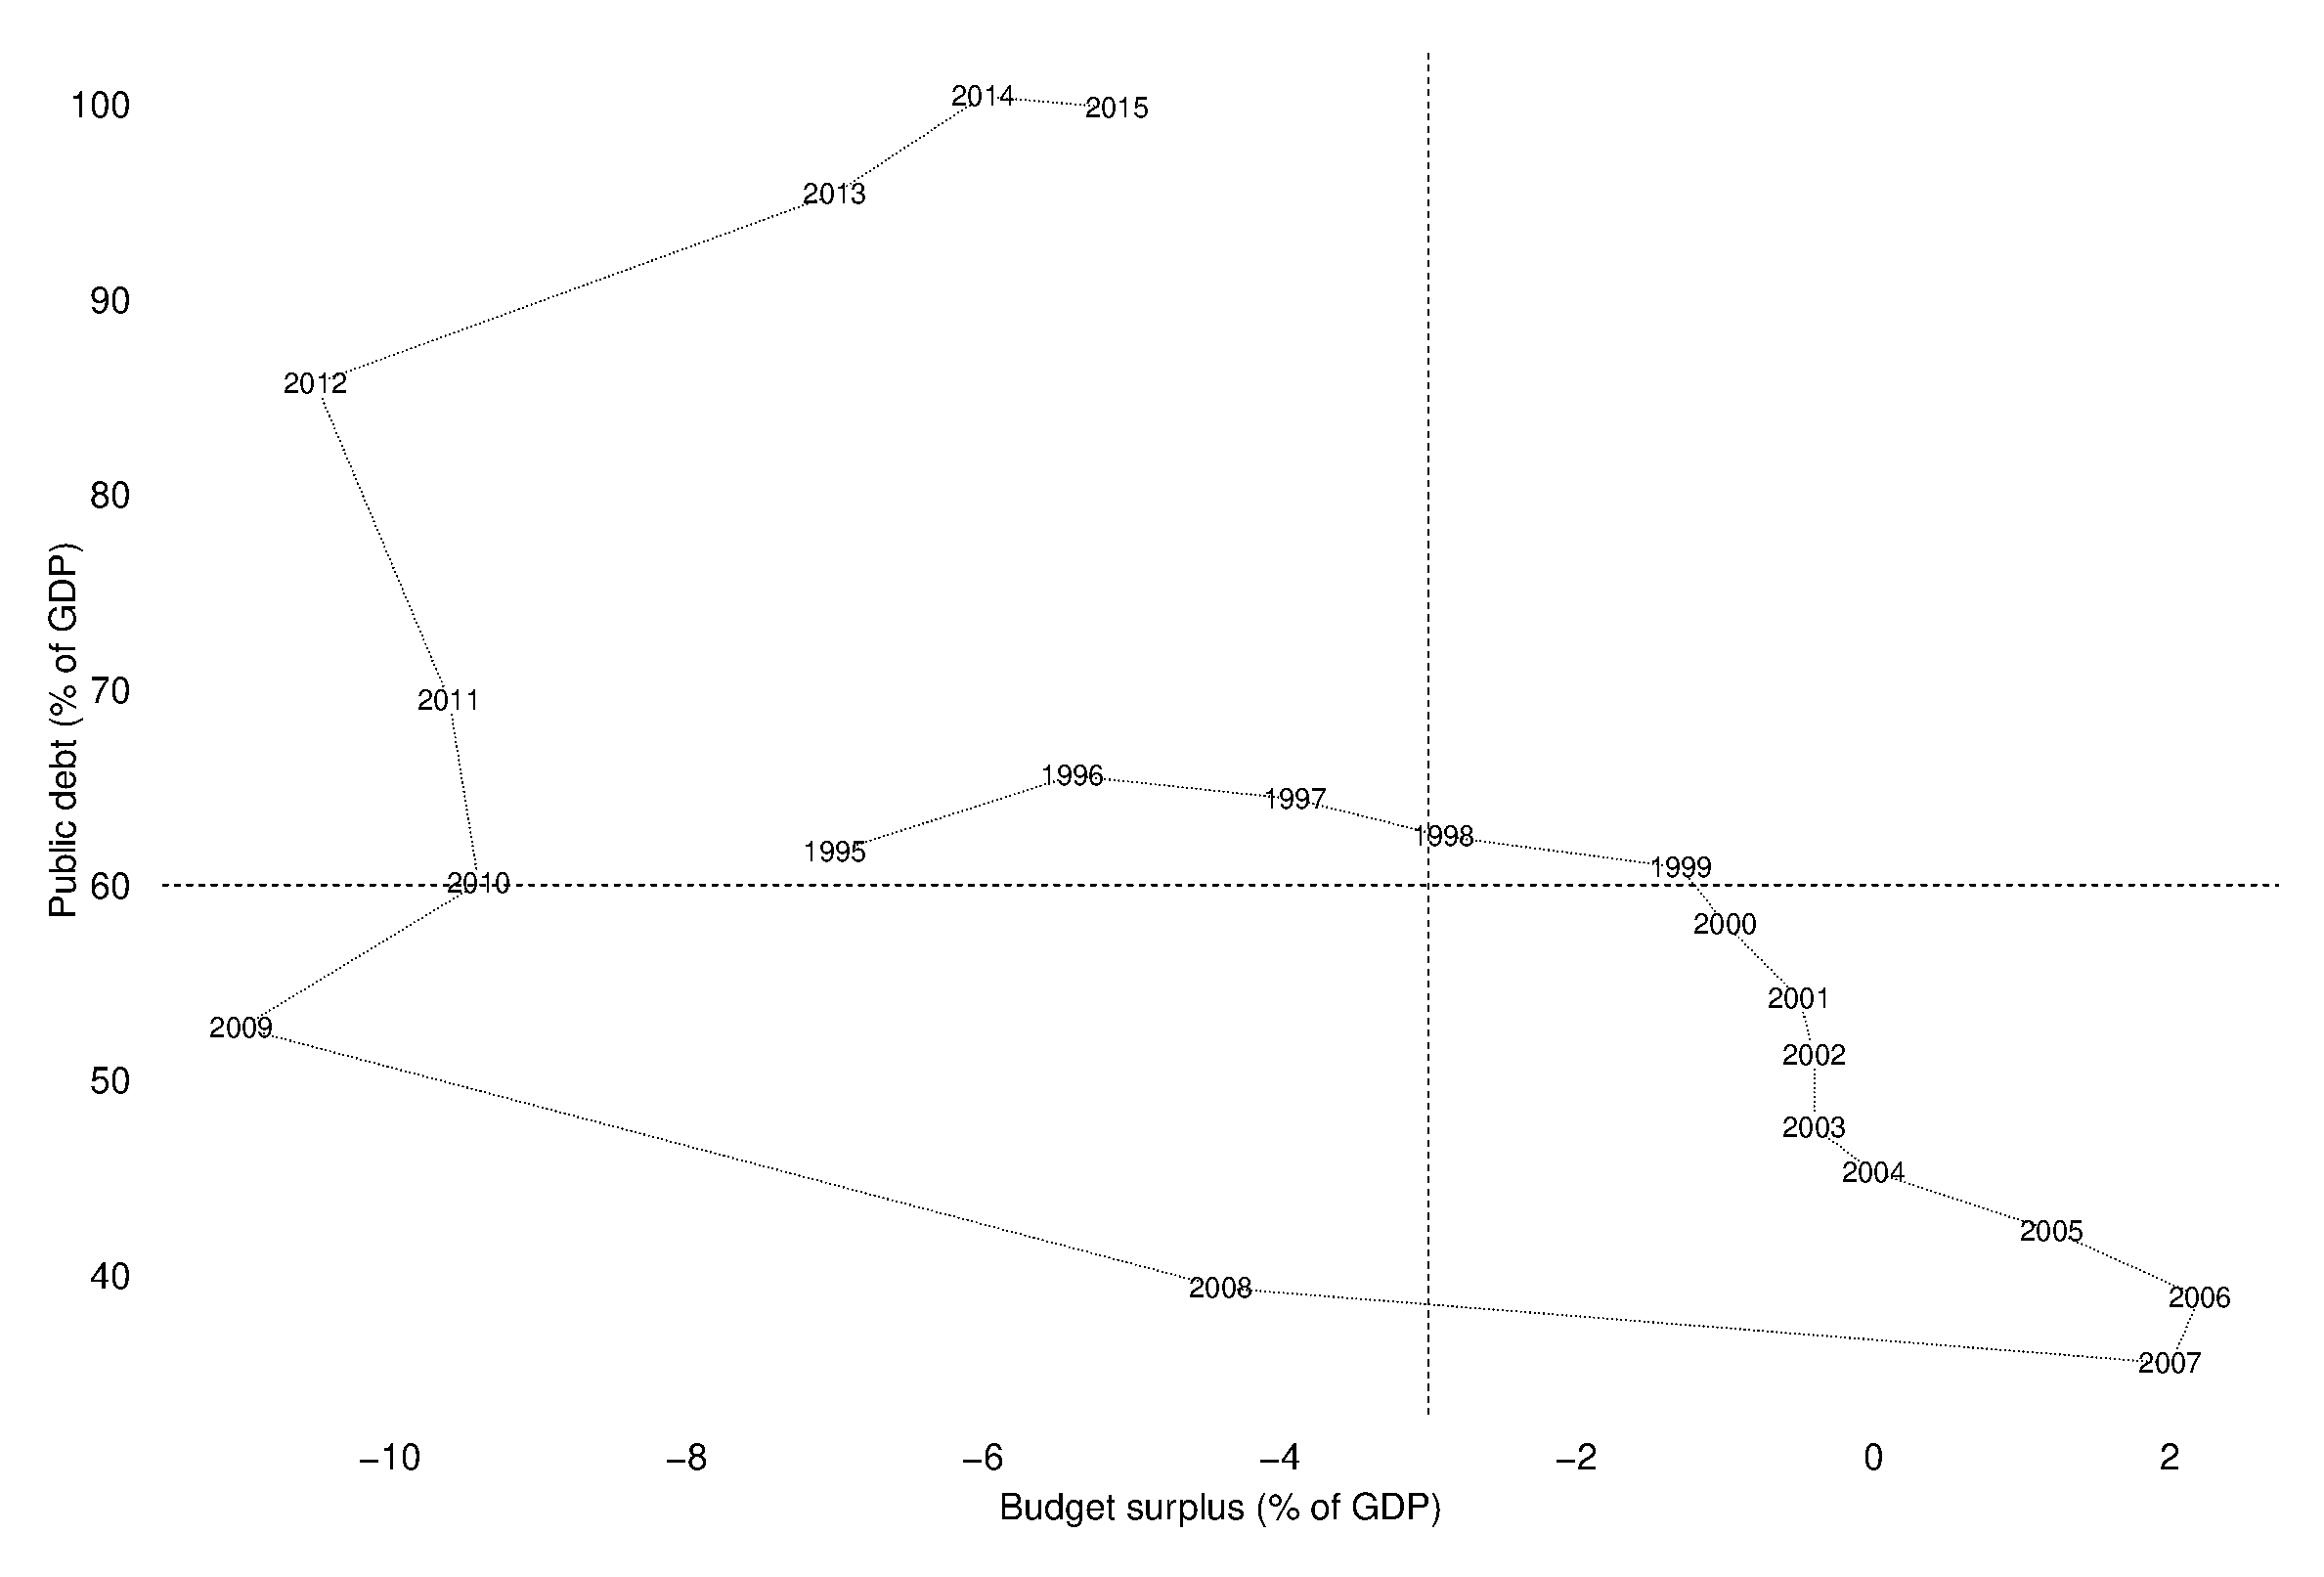
\includegraphics[scale=.3]{spain.eps}
  \end{figure}
\end{frame}
%--------------------------------------

%--------------------------------------
\begin{frame}
  \begin{figure}
    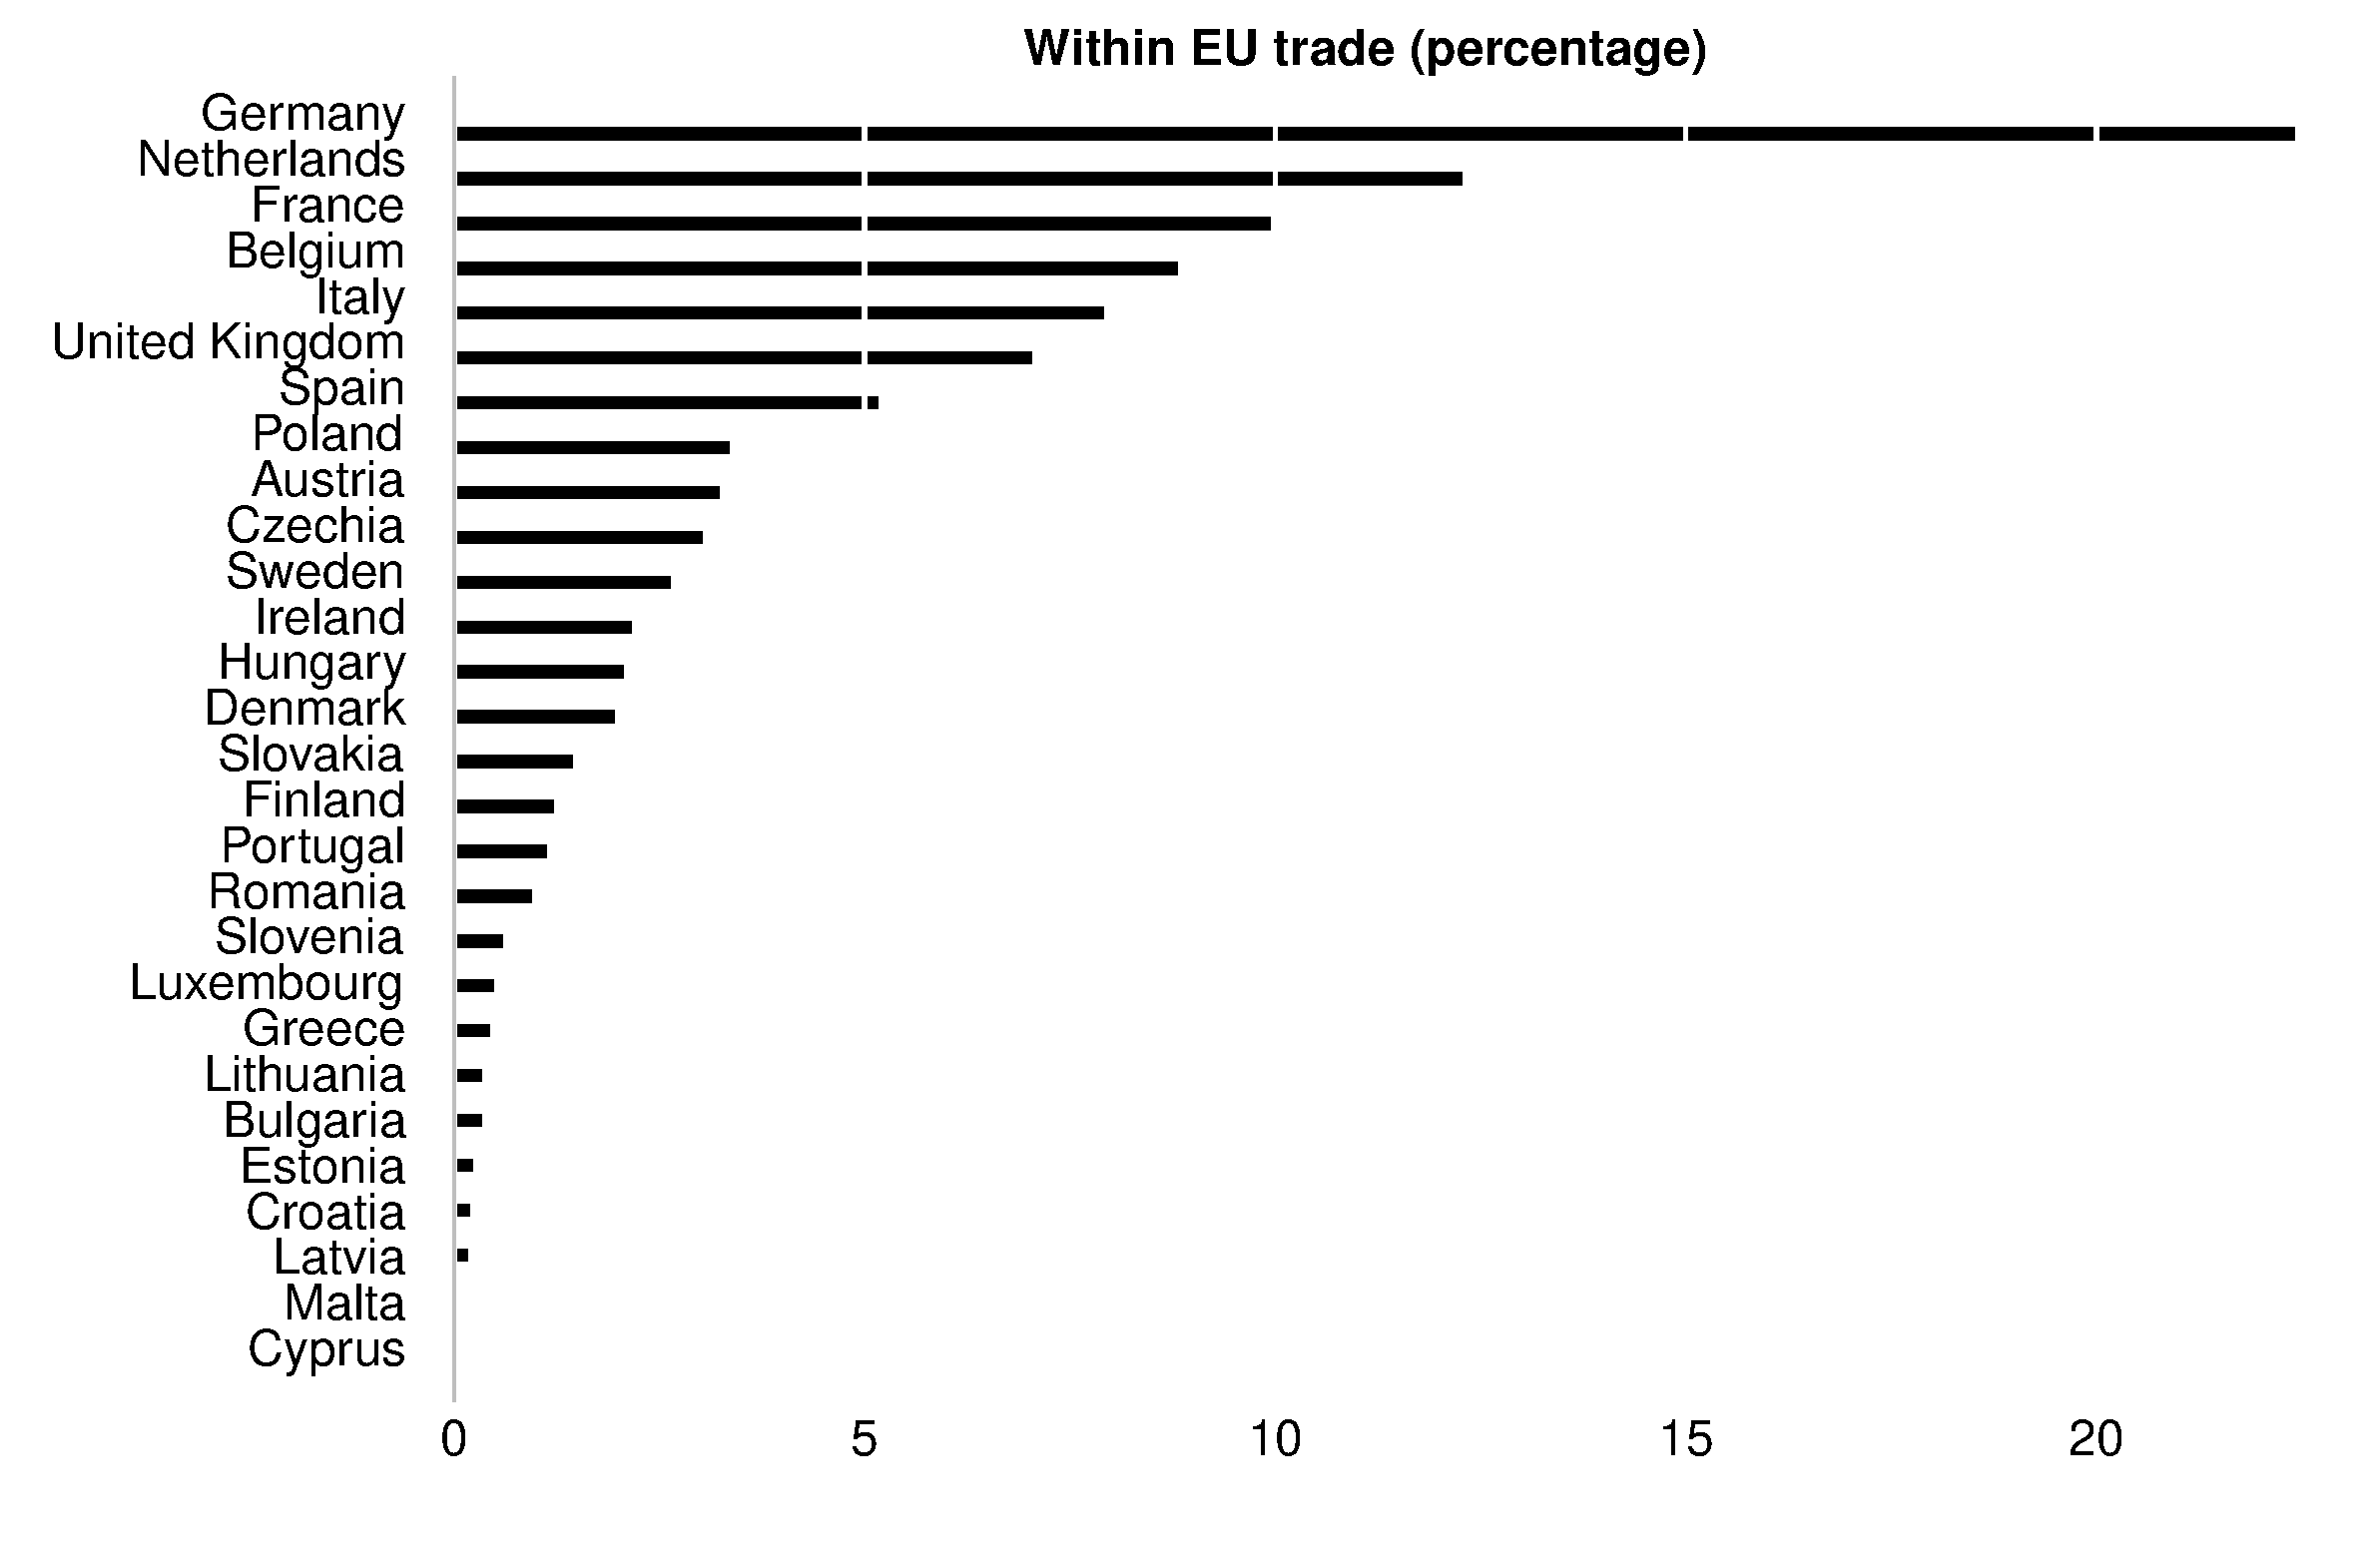
\includegraphics[scale=.3]{within_trade.eps}
  \end{figure}
\end{frame}
%--------------------------------------

%--------------------------------------
\begin{frame}
  \textbf{Trade imbalances}\\
  Cheap credit allowed countries to buy on loans
  \begin{itemize}
    \item Germany increase in trade surplus
    \item Italy, Spain, etc. increase in trade deficit
  \end{itemize}
  \medskip
  Eurozone peripheral areas rack up debts buy German goods: don't have money to pay for goods  
  \begin{itemize}
    \item Germany could export relatively cheaply because euro kept prices artificially low since it didn't appreciate
  \end{itemize}
\end{frame}
%--------------------------------------

%--------------------------------------
\begin{frame}
  \begin{figure}
    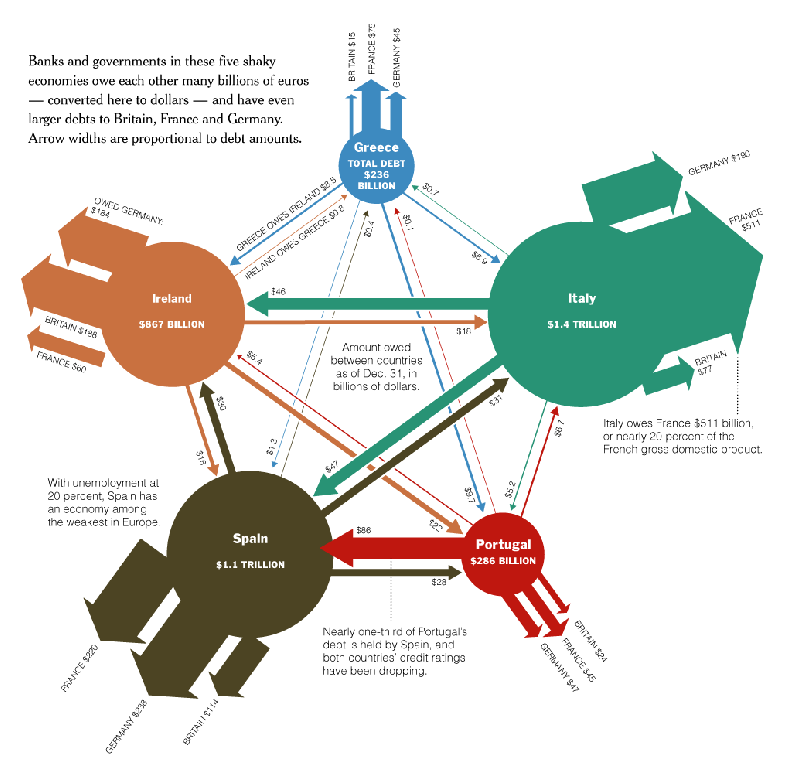
\includegraphics[scale=.6]{debt_nyt.eps}
  \end{figure}
\end{frame}
%--------------------------------------

%--------------------------------------
\begin{frame}
  \textbf{Debt and deficit}\\
  Straightforward that debt is caused by budget deficits, but how does this work in relation to GDP?\\
  \medskip
  Let $B_t$ be debt at end of year $t$ in nominal terms\\
  $D_t$ is deficit and will equal
  \begin{align}
    B_t-B_{t-1}=D_t
 \end{align}  
  \medskip
  Relative to GDP $Y$ we get  
  \begin{align}
    \frac{B_t-B_{t-1}}{Y_t} &= \frac{D_t}{Y_t}\\
    b_t-\frac{B_{t-1}}{Y_t} &= d_t    
  \end{align}
\end{frame}
%--------------------------------------

%--------------------------------------
\begin{frame}
 Can write GDP growth as
 \begin{align}
   g_t=\frac{Y_t-Y_{t-1}}{Y_{t-1}}=\frac{Y_{t}}{Y_{t-1}}-1
 \end{align}
 \medskip
 Can write
 \begin{align}
   \frac{B_{t-1}}{Y_t} = \frac{B_{t-1}}{Y_{t-1}} \cdot \frac{Y_{t-1}}{Y_t} = \frac{b_{t-1}}{1+g_t}  
 \end{align}  
\end{frame}
%--------------------------------------

%--------------------------------------
\begin{frame}
  \begin{align}
    b_t-\frac{b_{t-1}}{1+g_t} &= d_t\\ \nonumber
  b_t-b_{t-1} &= (1+g_t)d_t-g_tb_t  
  \end{align}
  \medskip
  Constant debt-to-GDP ratio requires
  \begin{align}
    b_t=b_{t-1}
  \end{align}
  \medskip Implies deficit-to-GDP ratio equaling 
\begin{align}
  (1+g_t)d_t-g_tb_t &=0 \\ \nonumber
  dt &= \frac{g_tb_t}{1+g_t} = \frac{g_t}{1+g_t}b_t
\end{align}
\end{frame}
%--------------------------------------


%--------------------------------------
\begin{frame}
  Maastricht Treaty has set convergence criteria to
  \begin{align*}
    b_t=60\%\\
    d_t=3\%
  \end{align*}
  \medskip
  Therefore, $g$ needs to equal about 5.3\%
   \begin{itemize}
     \item Implicit assumption: real GDP growth of 3\%, inflation  2\%, equaling a nominal growth rate of 5\%.  
   \end{itemize} 
   \medskip
   If a country is able to keep the debt level constant then naturally the debt-to-GDP ratio will decrease due to GDP growth. 
   \begin{itemize}
     \item This also implies that the deficit becomes larger at high nominal growth rates.  
   \end{itemize}
\end{frame}
%--------------------------------------


%--------------------------------------
\begin{frame}
  \textbf{EU response}\\
  Economic problem required solution with political backing
  \begin{itemize}
    \item Not easy given break down in confidence between member states: specifically North vs. South    
  \end{itemize}
  \medskip
  Some solutions that didn't make it
  \begin{enumerate}
    \item Eurobonds
    \item Fiscal transfers
    \item Grexit
    \item Quantitative Easing (QE)
  \end{enumerate}
 \end{frame}
%--------------------------------------

%--------------------------------------
\begin{frame}
  \textbf{Eurobonds}
  \begin{itemize}
    \item Allows government to refinance debts: high-yield countries benefit from creditworthiness low-yield countries
    \item Moral hazard problem
  \end{itemize}
  \medskip
  \textbf{Fiscal transfers}
  \begin{itemize}
    \item Richer countries pay poorer countries (peripheraid, permanent bail out)
    \item No system in place to do this: would need political backing;  unlikely to be popular with population of richer countries    
  \end{itemize}
\end{frame}
%--------------------------------------

%--------------------------------------
\begin{frame}
  \begin{figure}
    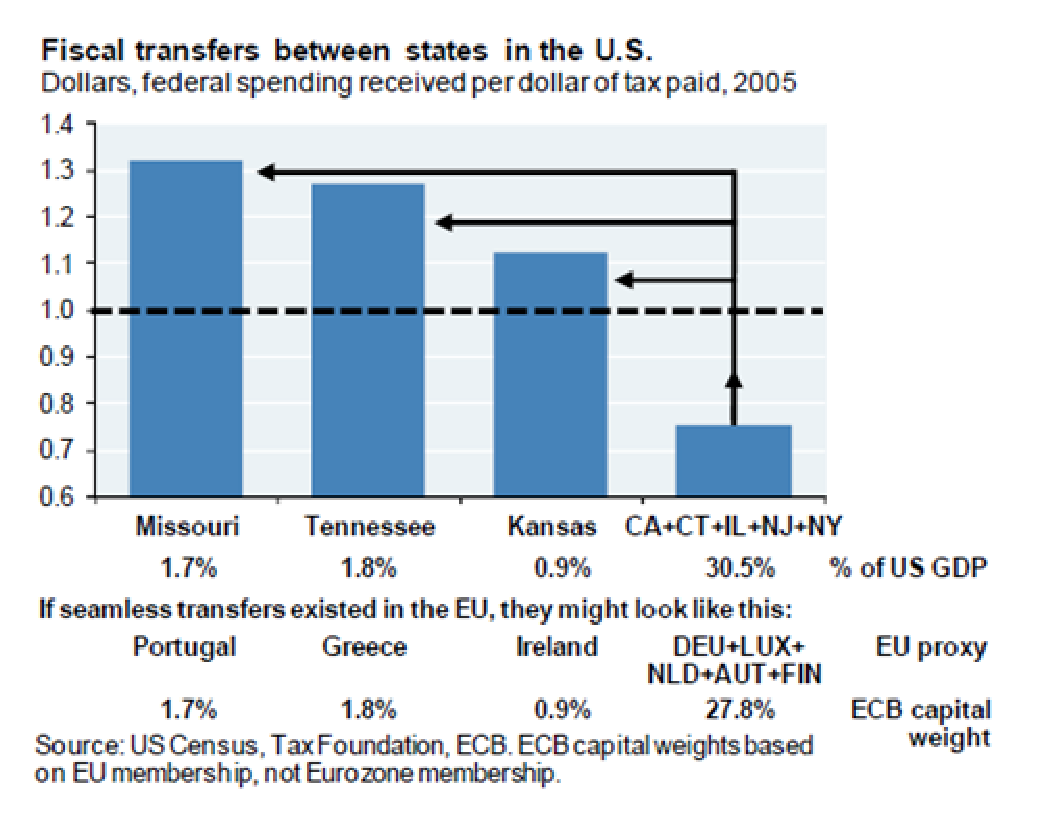
\includegraphics[scale=.6]{peripheraid.eps}
  \end{figure}
\end{frame}
%--------------------------------------

%--------------------------------------
\begin{frame}
  \textbf{Grexit}
  \begin{itemize}
    \item Return to drachme: Greece would be able to set own monetary policy and regain competitiveness    
    \item Would create undesired precedent and risk stability of the whole euro project
  \end{itemize}
  \medskip
  \textbf{QE}
  \begin{itemize}
    \item Help boost economic activity (e.g. Japan)
    \item Germany not a fan (ECB did engage in form of QE eventually)    
  \end{itemize}
\end{frame}
%--------------------------------------

%--------------------------------------
\begin{frame}
  EU took following measures (2010)
  \begin{itemize}
    \item European Financial Stability Facility (EFSF) 
    \item European Financial Stabilisation Mechanism (EFSM) 
  \end{itemize}
  \medskip
  More or less temporary measures followed up by a more formalised structure to assist eurozone member states under the European Stability Mechanism (ESM) in 2012.
\end{frame}
%--------------------------------------

%--------------------------------------
\begin{frame}
  \textbf{European Financial Stability Facility}\\
  Temporary crisis resolution mechanism for euro area member states financed through the issuance of bonds and other debt instruments
  \begin{itemize}
    \item Capacity of 500B EU
    \item Guaranteed by other eurozone member states (so sort of eurobonds)
  \end{itemize}
    \medskip
   Assistance was used to provide loans, recapitalise banks, or buy sovereign debt    
   \begin{itemize}
     \item For Ireland, Portugal, Greece
   \end{itemize}
\end{frame}
%--------------------------------------

%--------------------------------------
\begin{frame}
  \textbf{European Financial Stabilisation Mechanism}\\
   Provides financial assistance to any EU member state which is facing severe financial disturbances
   \begin{itemize}
     \item Country can get up to 60B EUR in assistance from the European Commission 
     \item The fund is financed through  bond sales, using EU budget as collateral    
    \item Provided assistance to Ireland and Portugal, and a short term loan to Greece
   \end{itemize}
\end{frame}
%--------------------------------------

%--------------------------------------
\begin{frame}
  \textbf{European Stability Mechanism}\\
  Aimed to help overcome the problem for countries facing a debt crisis that they couldn't get credit from international financial markets or at unfavourable rates
  \begin{itemize}
    \item Basically extension of EFSF
  \end{itemize}
  Budget of 700B EUR
  Between 2012-2016, the programme disbursed about 250B EUR to five countries
\begin{itemize}
  \item Ireland, Portugal, Greece (2x), Spain, Cyprus February 2011 (part of EFSF)
\end{itemize}
\end{frame}
%--------------------------------------

%--------------------------------------
\begin{frame}
  \textbf{The Greek Depression}\\
  Focal point of eurocrisis when it emerged in late 2009 that they had been understating their debt figures
  \begin{itemize}
    \item Misreported numbers at Eurostat
    \item Led to serious doubts about the state of the Greek economy and government finances in particular leading to high yields on its bonds, effectively barring the country from lending money on the international market.
  \end{itemize}
  \medskip
  Although the country experienced a substantial period of growth from 1995 onwards, the crisis destroyed much of the progress made over the years with current GDP being at the level of 2000.
\end{frame}
%--------------------------------------

%--------------------------------------
\begin{frame}
  \scalebox{.7}{
  \begin{quote}
    Greece is an important country in the European Union, given its history in Europe, its strategic position in the Eastern Mediterranean, and its potential
in the services industries. Europe’s commitment to Greece is manifested in the heavy transfers it makes every year. It is in Europe’s interest to wean countries like Greece and Portugal from these transfer payments and the best chance to do so is to help Greece to establish the conditions for bringing its economy into macroeconomic balance. That could best be achieved by allowing Greece to enter the EMU. If 14 countries were to qualify for EMU, and Greece made a concerted effort to bring its economy into balance, the marginal cost of allowing Greece to enter would be small compared to its huge benefits
  \end{quote}}
   \textbf{Mundell} (1997)
\end{frame}
%--------------------------------------

%--------------------------------------
\begin{frame}
  \begin{figure}
    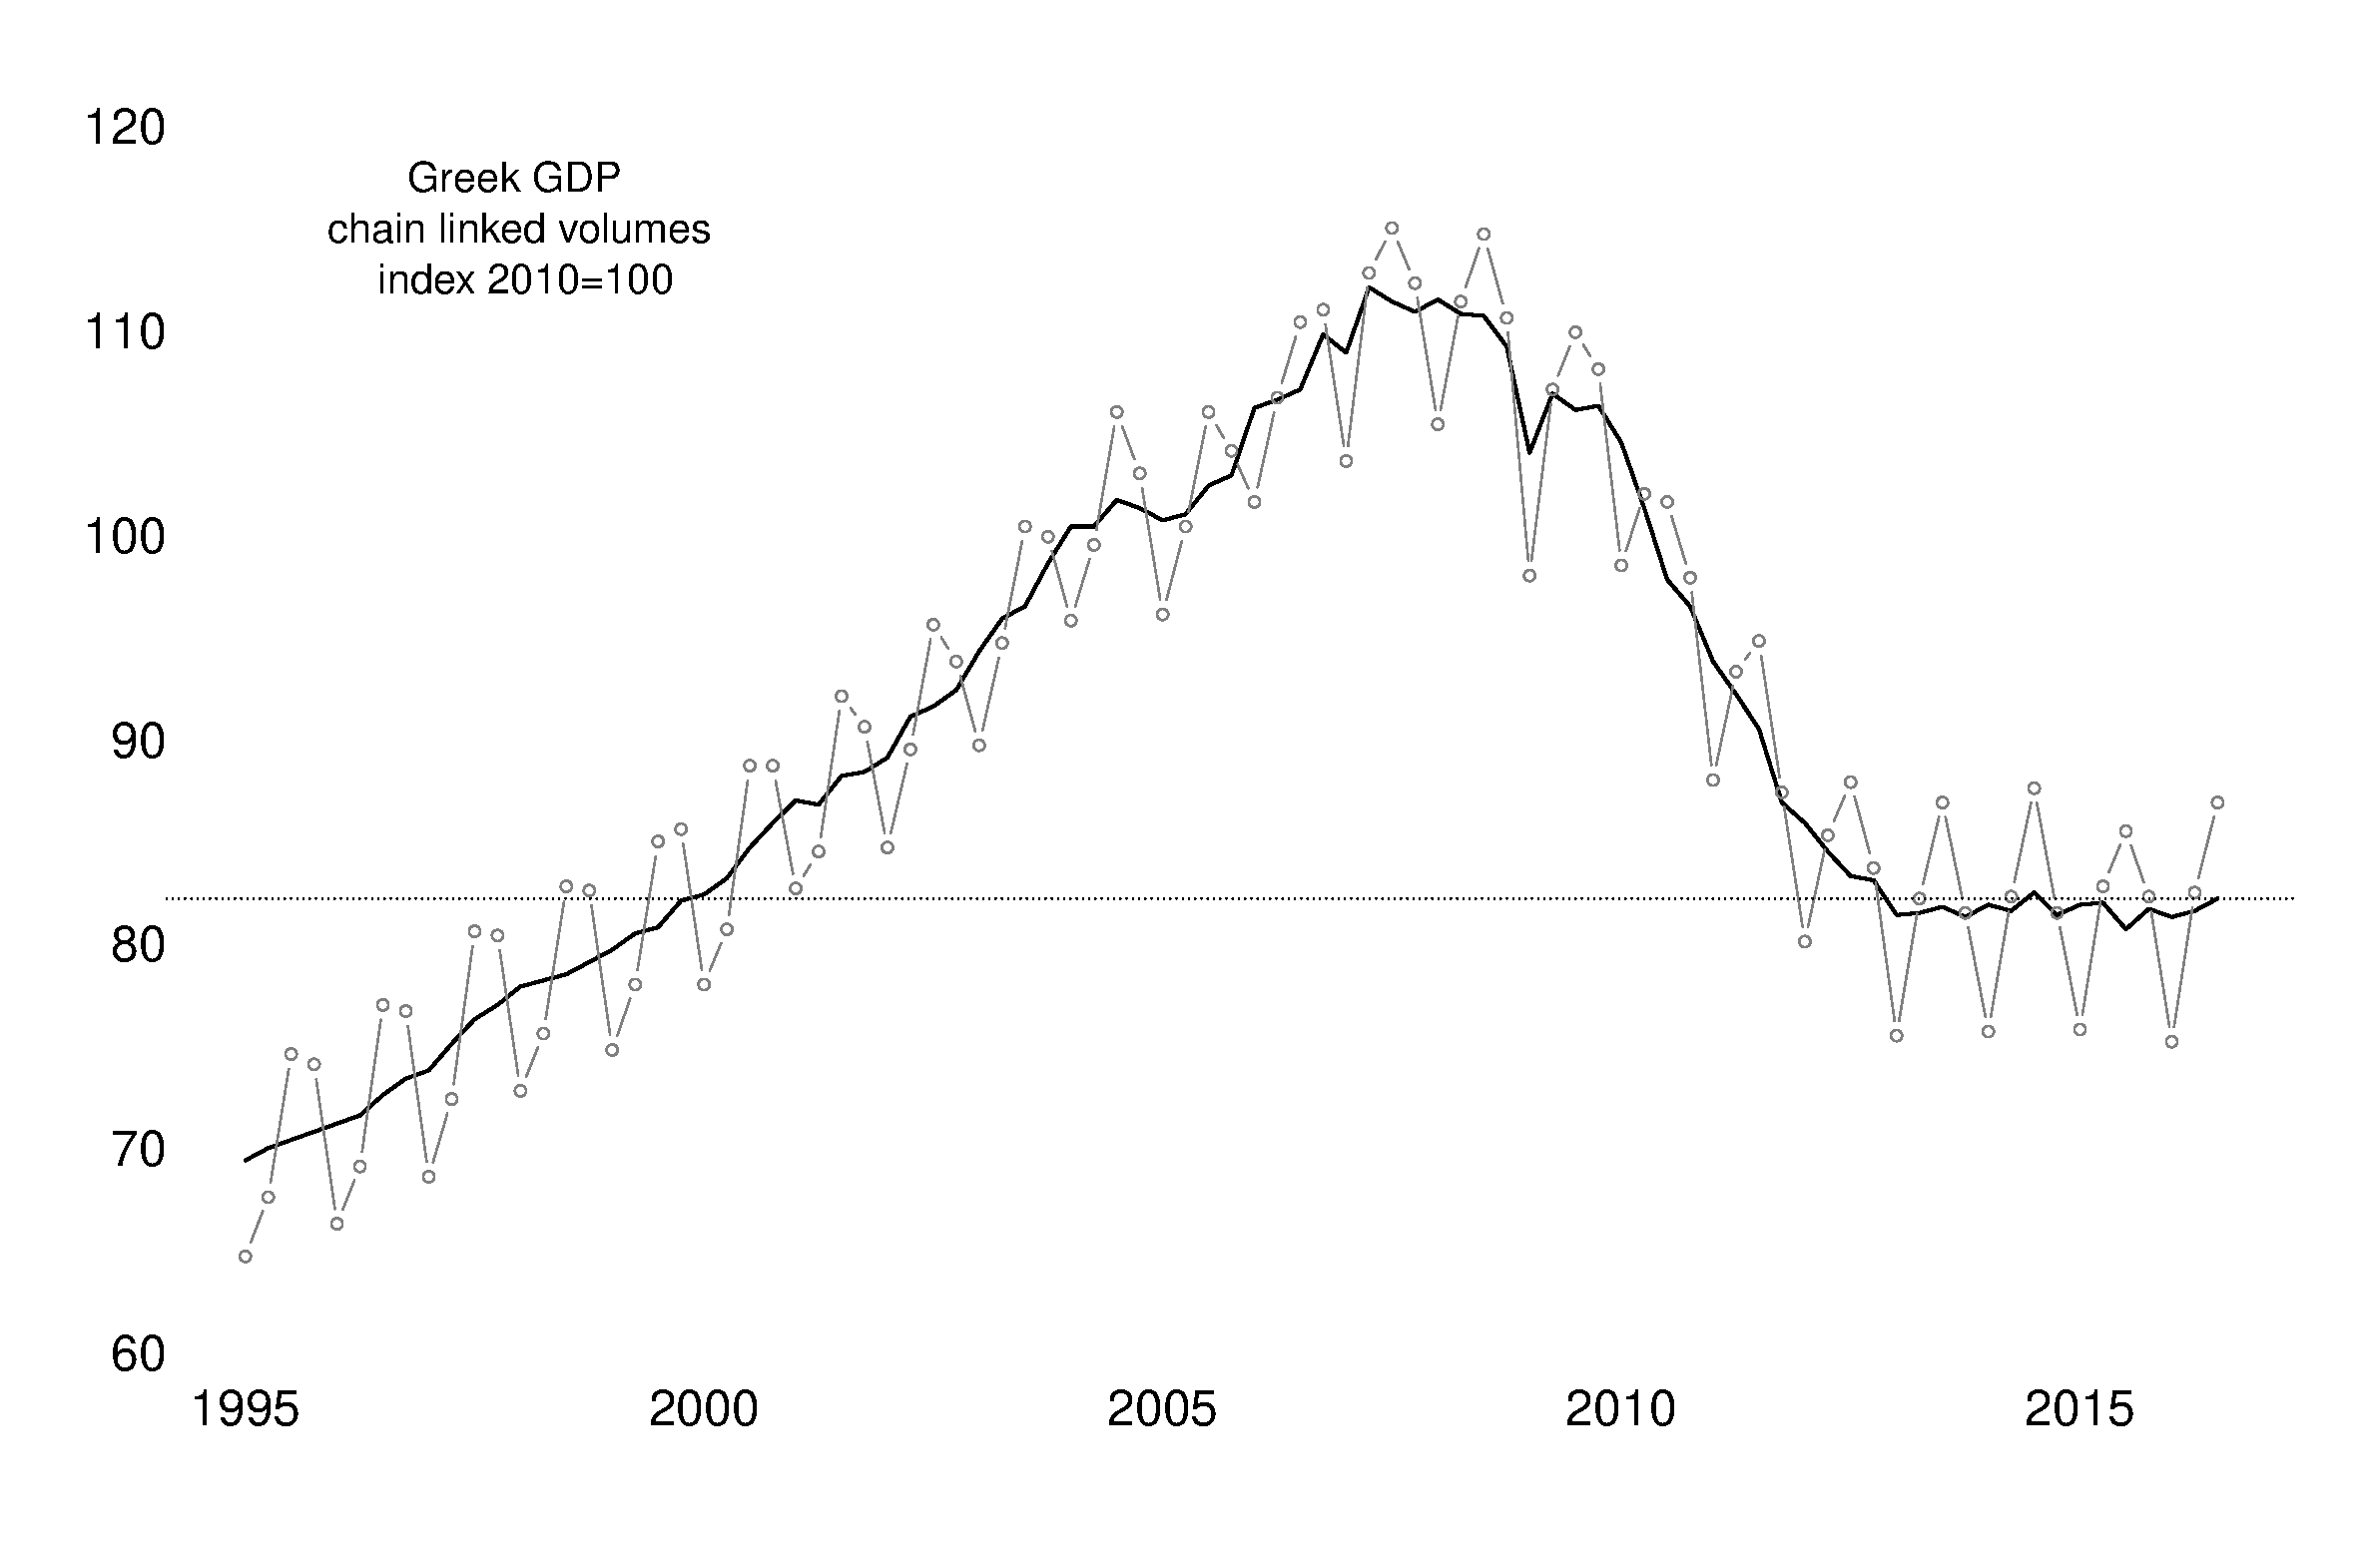
\includegraphics[scale=.3]{greece1.eps}
  \end{figure}
\end{frame}
%--------------------------------------

%--------------------------------------
\begin{frame}
  \begin{figure}
    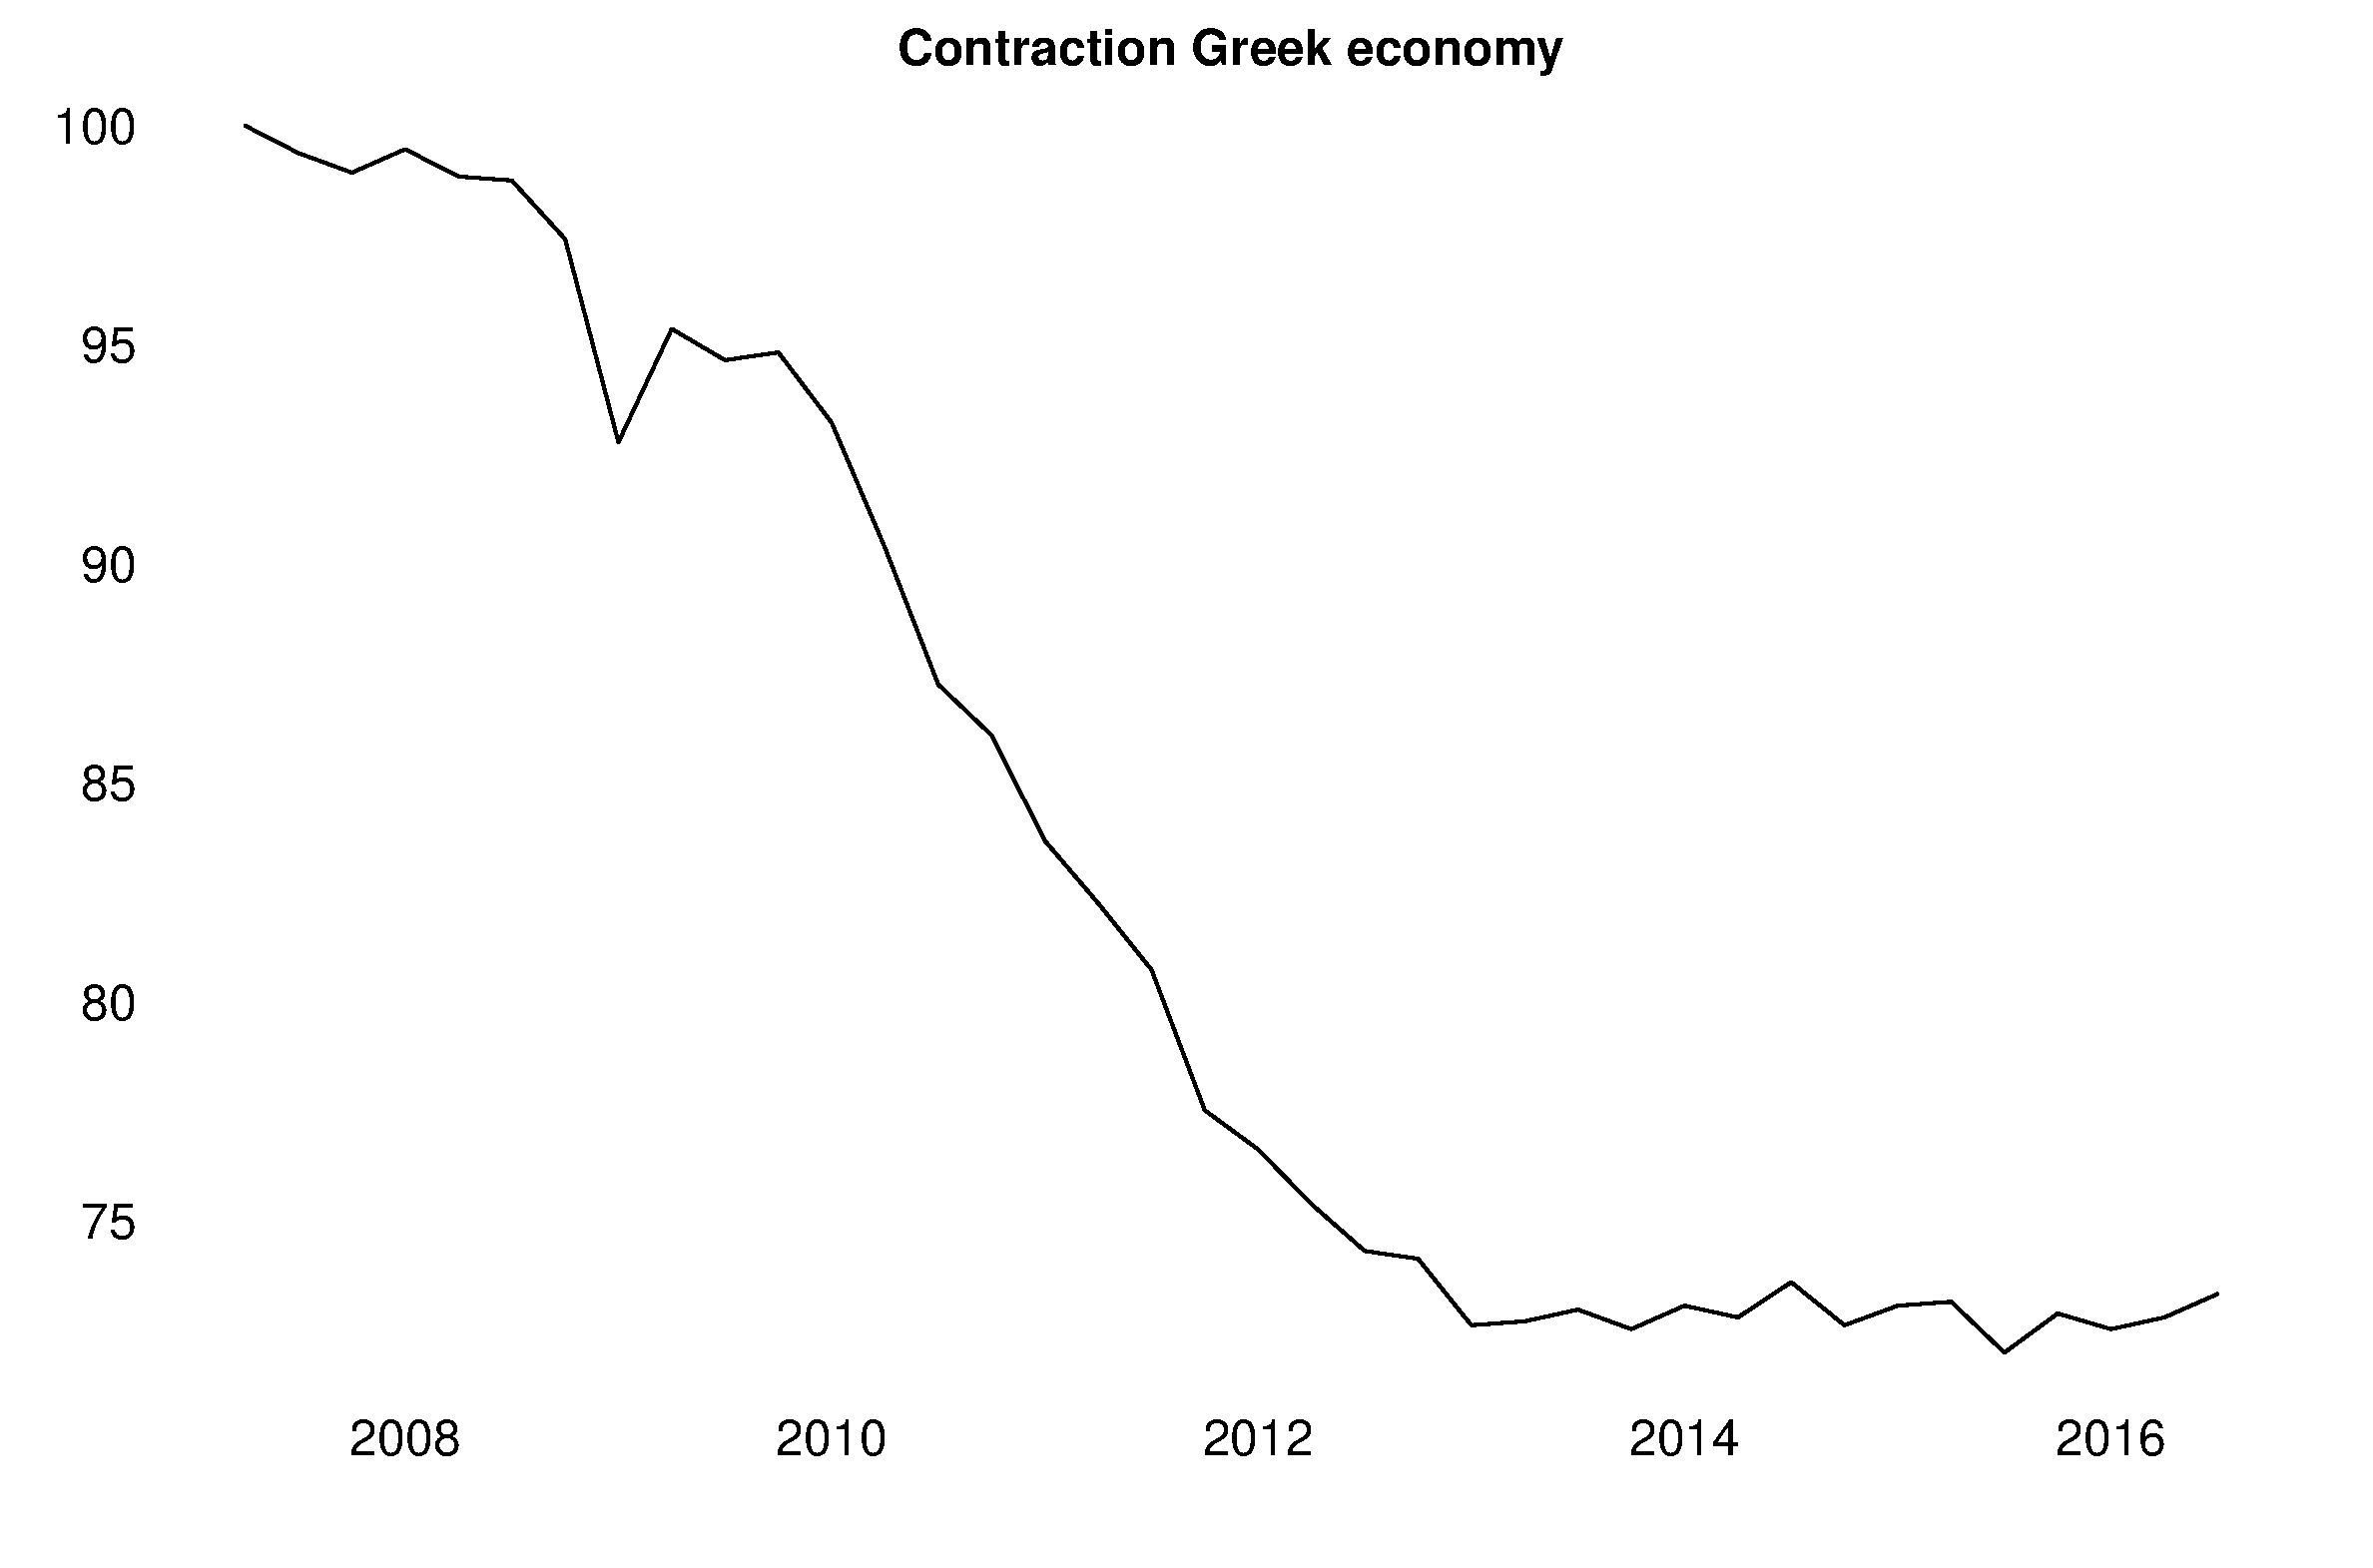
\includegraphics[scale=.3]{greece2.eps}
  \end{figure}
\end{frame}
%--------------------------------------

%--------------------------------------
\begin{frame}
  \textbf{Debt reduction schemes}
  \begin{enumerate}
    \item Unilateral debt forgiveness
    \item Third party buy-backs
    \item Debt restructuring (haircut)
    \item Debt swaps
    \item Default (nuclear option)
  \end{enumerate}  
\end{frame}
%--------------------------------------

%--------------------------------------
\begin{frame}
  \textbf{Greek debt reduction scheme}
  \begin{itemize}
    \item \textbf{21 Jan. 2010} Greek-German spread for 10-y debt reaches 300 basis points
    \begin{itemize}
      \item Default only option without outside help
    \end{itemize}
    \item \textbf{2 May 2010} Troika agree to 140B EUR bail-out package
    \begin{itemize}
      \item Guarantee Greek public debt: debt swap
    \end{itemize}
    \item \textbf{27 Oct. 2011} Major private bond holders agree on haircut
    \begin{itemize}
      \item 50\%: 83.5\% of Greek bond holders participate
    \end{itemize}
    \item \textbf{2012-2014} Arrangement becomes third party buy-back: ECB buys out large fraction and lowers interest rates
  	\item \textbf{Feb. 2014} Greek debt/GDP >170\%: Greece hopes for debt forgiveness from Troika
  	\item \textbf{2015} Greece defaults on IMF loan
  \end{itemize}
\end{frame}
%--------------------------------------

%--------------------------------------
\begin{frame}
  \begin{figure}
    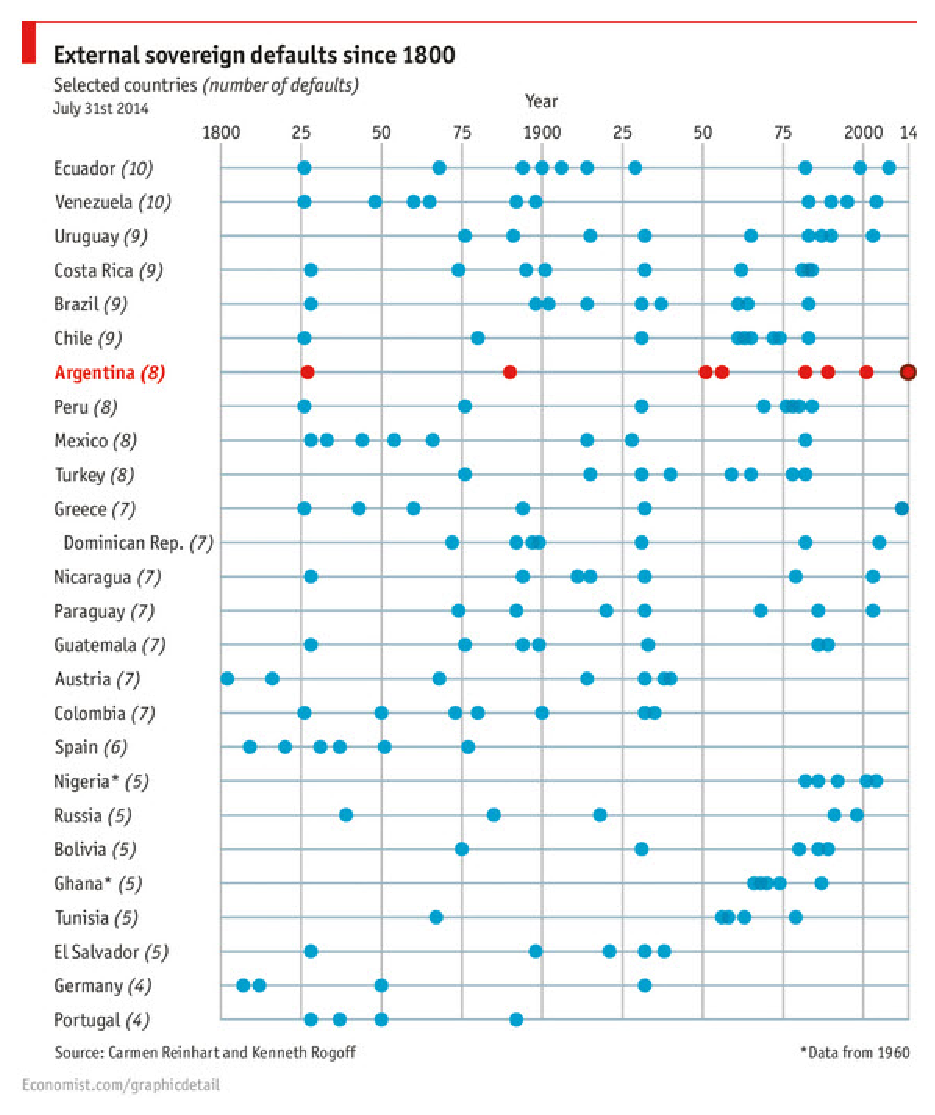
\includegraphics[scale=.5]{defaults.eps}
  \end{figure}
\end{frame}
%--------------------------------------

%--------------------------------------
\begin{frame}
  Consider country has $P(default)=0.1$ over next year; leading to 50\% default on outstanding debt
  \begin{itemize}
    \item Country needs to pay 5\% premium on debt relative to safe assets
  \end{itemize}
  \medskip
  Premium imposes additional burden on government
  \begin{itemize}
    \item Interest costs rise above the funds that country can access to pay off the interest payments
    \item Alternatively the country's GDP could expand in order to keep debt stable
  \end{itemize}
  Market for government bonds might cease to operate as the country is deemed not credit-worthy: risk goes from unlikely to likely
  \begin{itemize}
    \item Closing of a bond market is an rare and abrupt events: People often don't see it coming
  \end{itemize}
  After a default a country needs to restructure it debt which often involves writing off part of it, in order to restore the debt level to a more sustainable level. 
\end{frame}
%--------------------------------------

%--------------------------------------
\begin{frame}
  \textbf{Terms and conditions apply}
  \begin{itemize}
    \item Harsh austerity terms 
  \begin{itemize}
    \item Cuts in public spending such as investments 
    \item Tax increases    
  \end{itemize}
  \item Government overhaul
  \begin{itemize}
    \item Reducing size of the government apparatus
    \item Cutting back on pensions
    \item Importantly there were no cuts to defense spending in terms of percentage GDP    
  \end{itemize}
  \item Ending tax evasion by its citizens
  \item Making business in Greece easier  
  \end{itemize}
\end{frame}
%--------------------------------------

%--------------------------------------
\begin{frame}
  \begin{figure}
    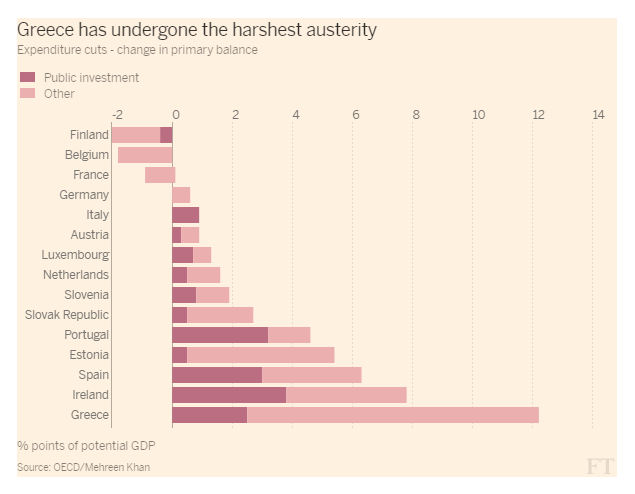
\includegraphics[scale=.8]{austerity.eps}
  \end{figure}
\end{frame}
%--------------------------------------

%--------------------------------------
\begin{frame}
  \begin{figure}
    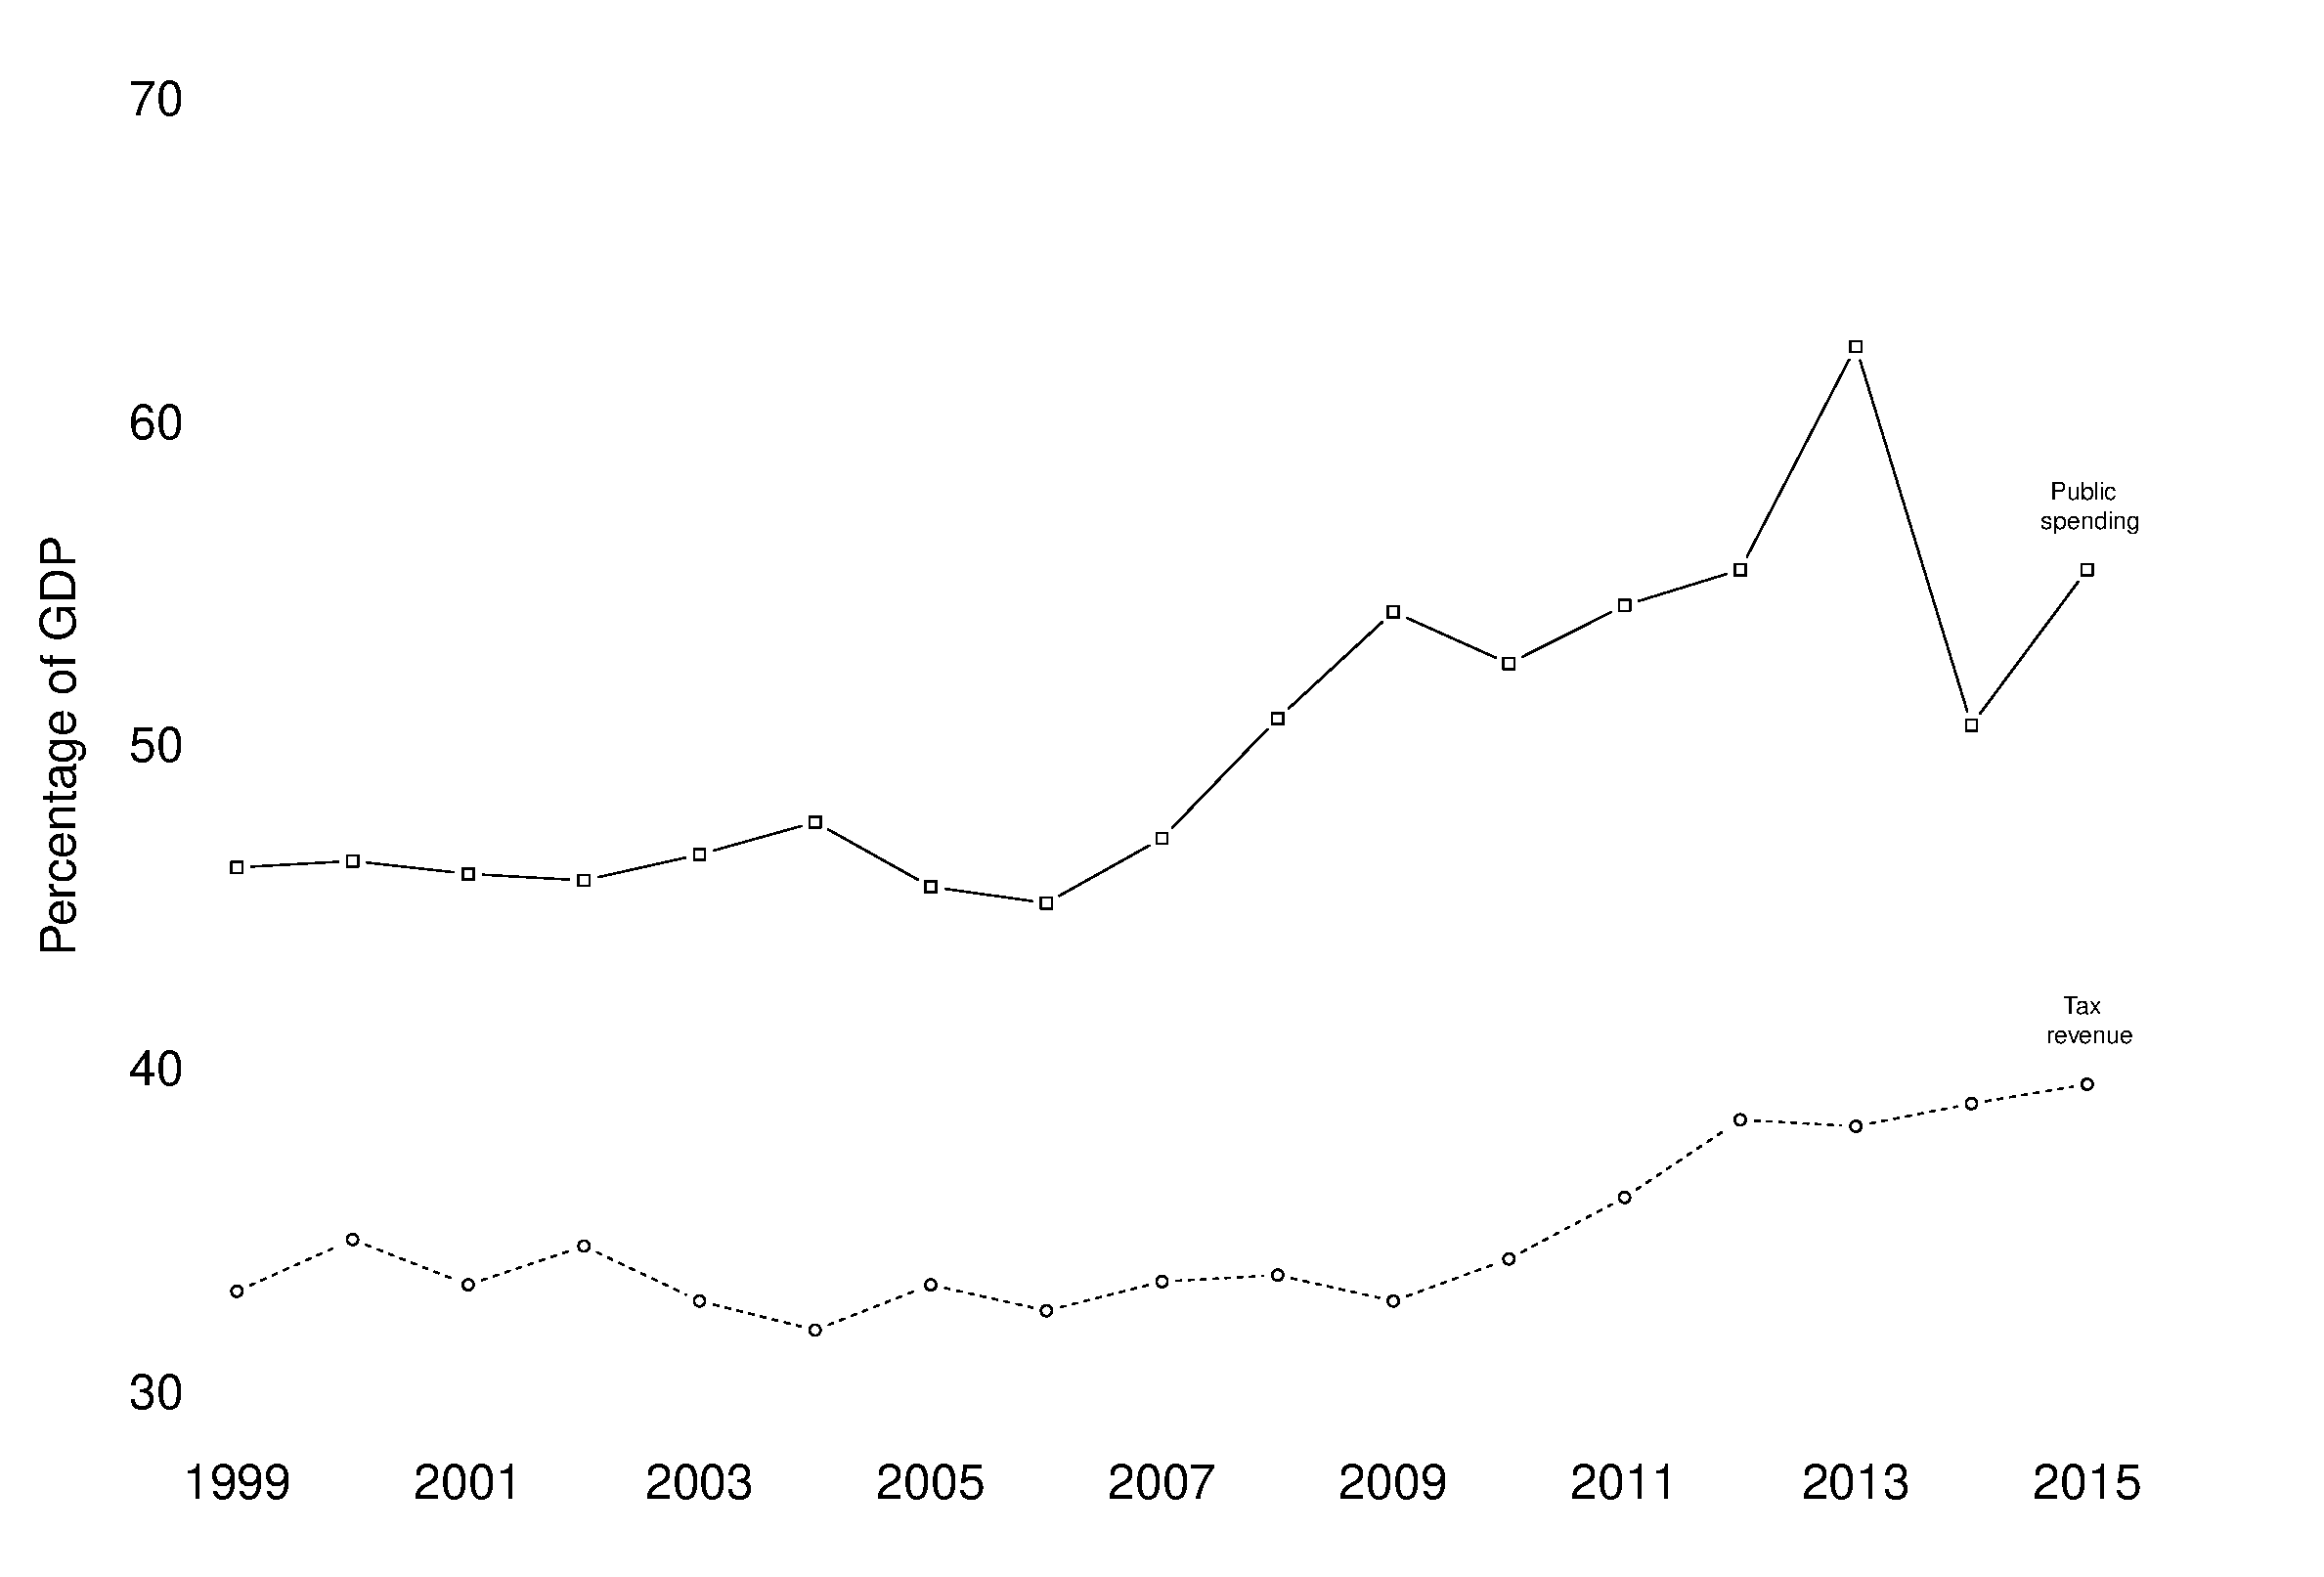
\includegraphics[scale=.3]{greece3.eps}
  \end{figure}
\end{frame}
%--------------------------------------

%--------------------------------------
\begin{frame}
  \begin{figure}
    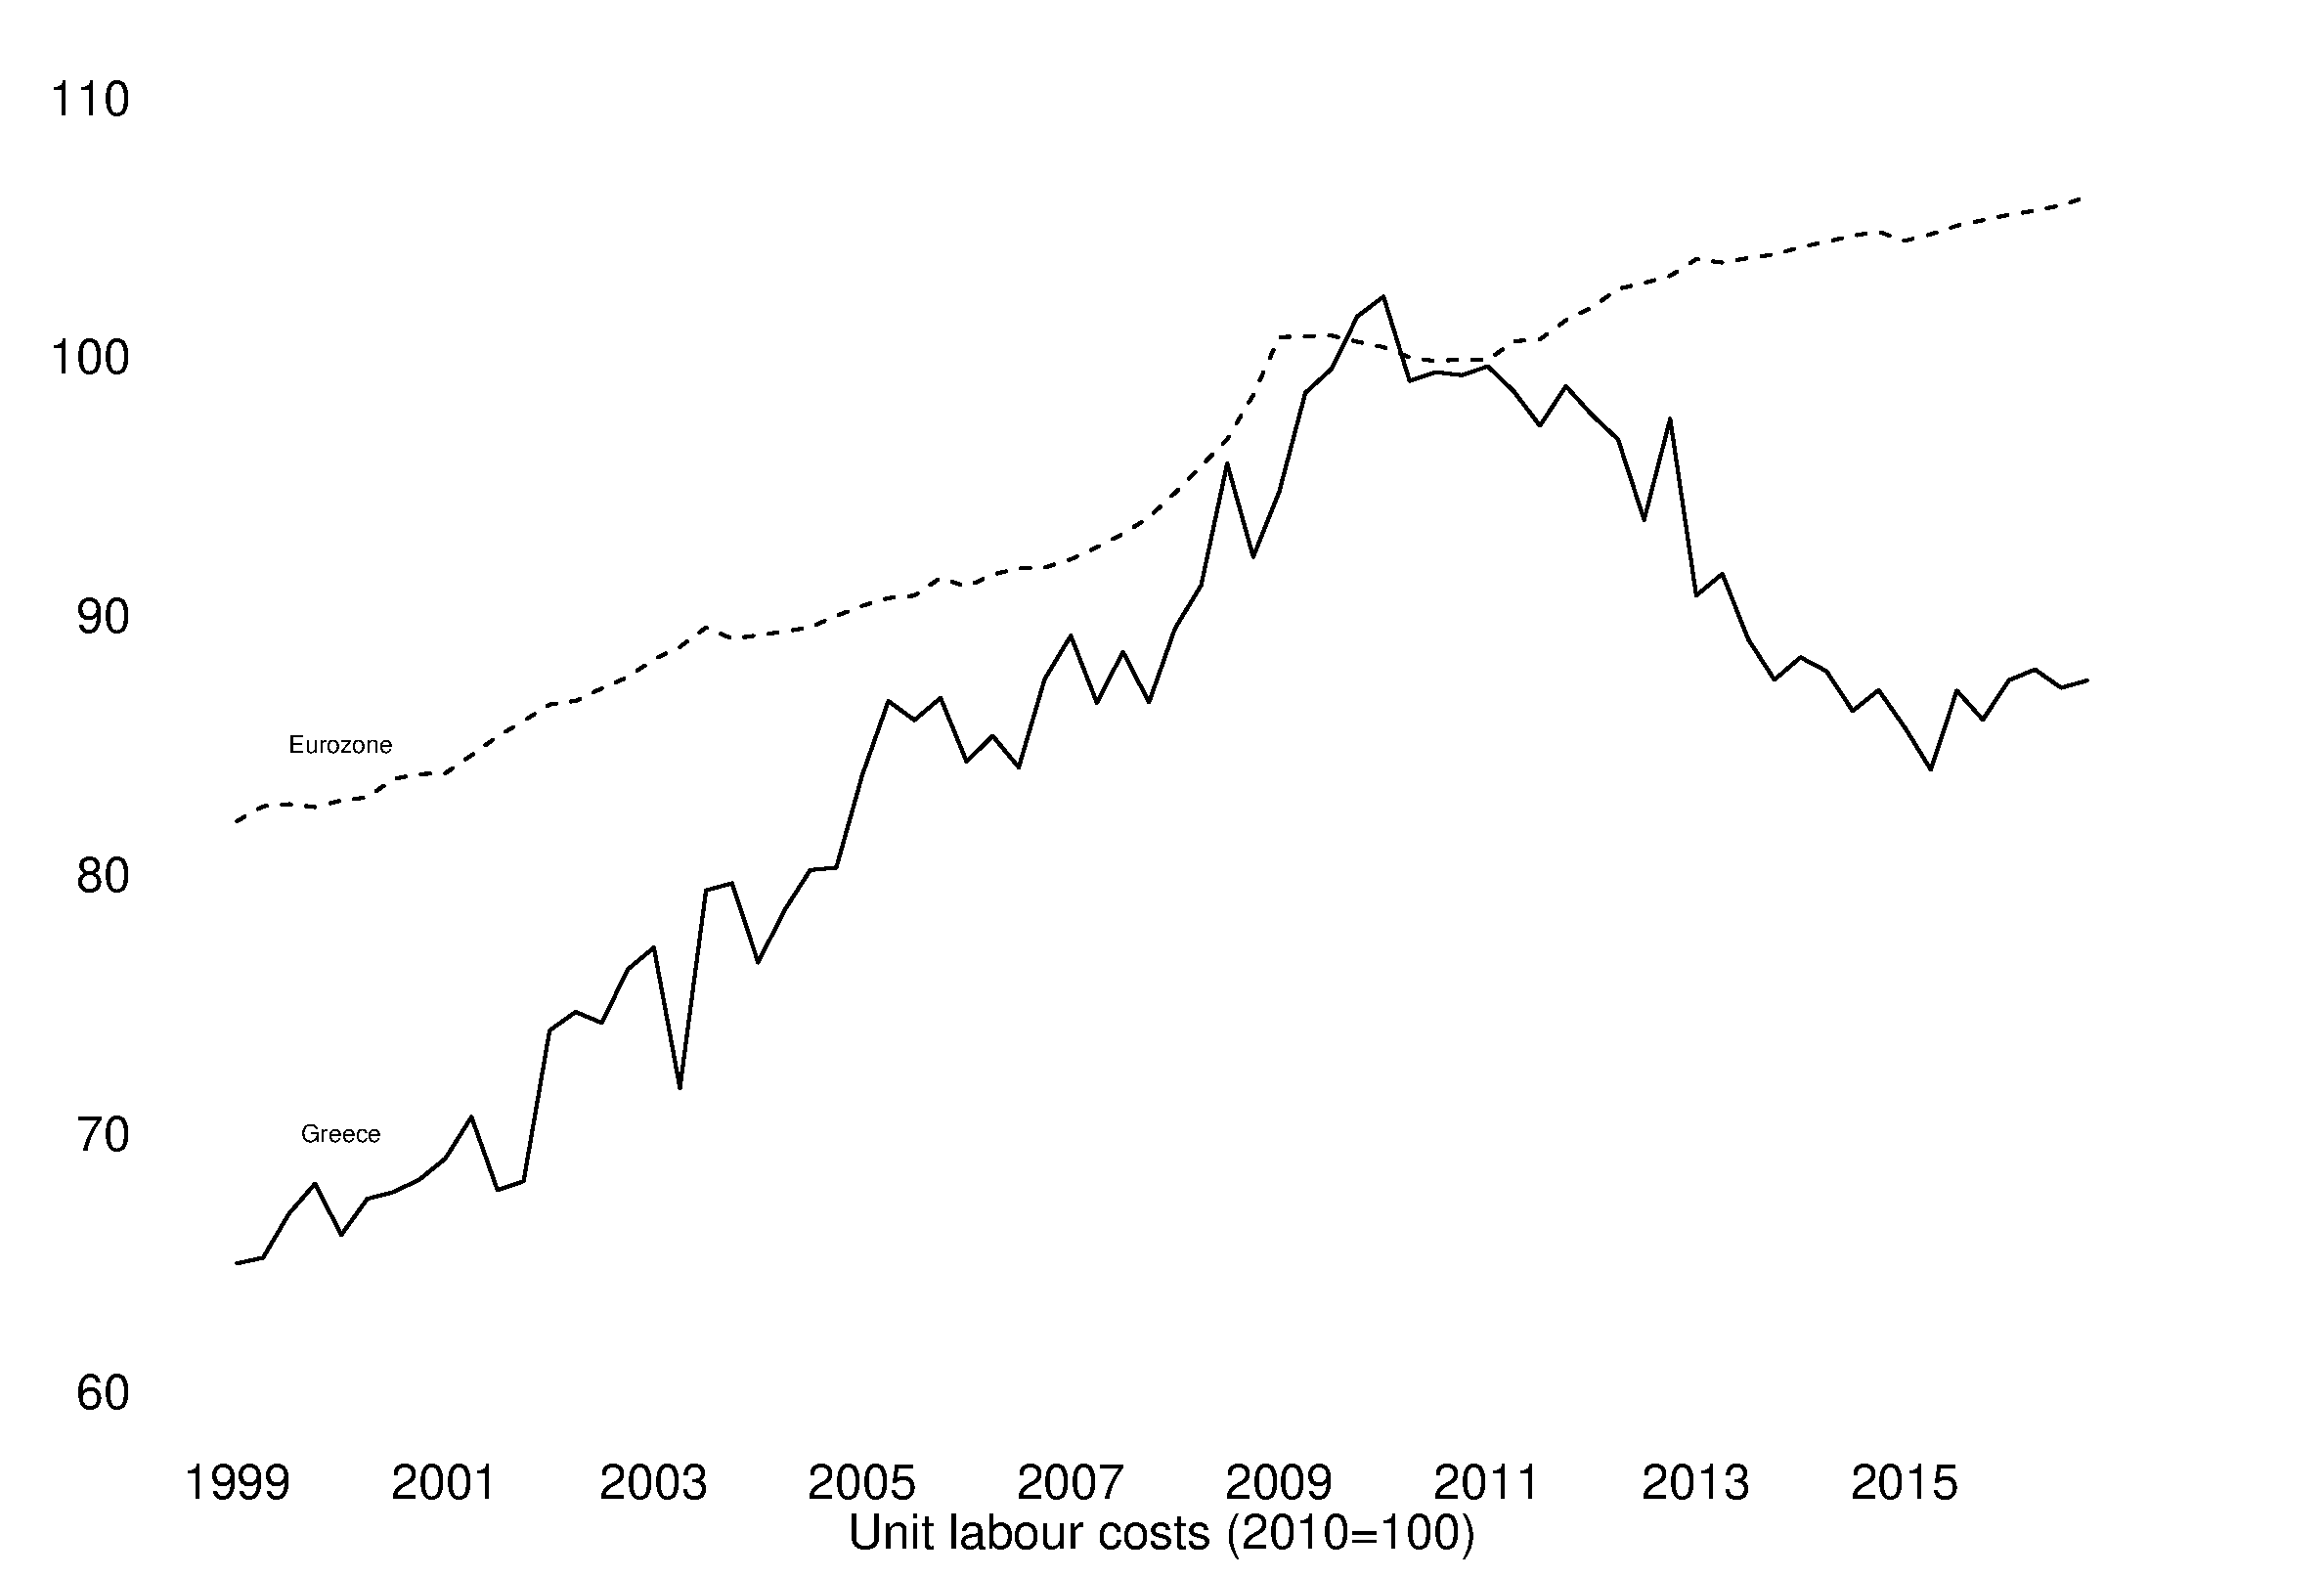
\includegraphics[scale=.3]{greece4.eps}
  \end{figure}
\end{frame}
%--------------------------------------

%--------------------------------------
\begin{frame}
  \begin{figure}
    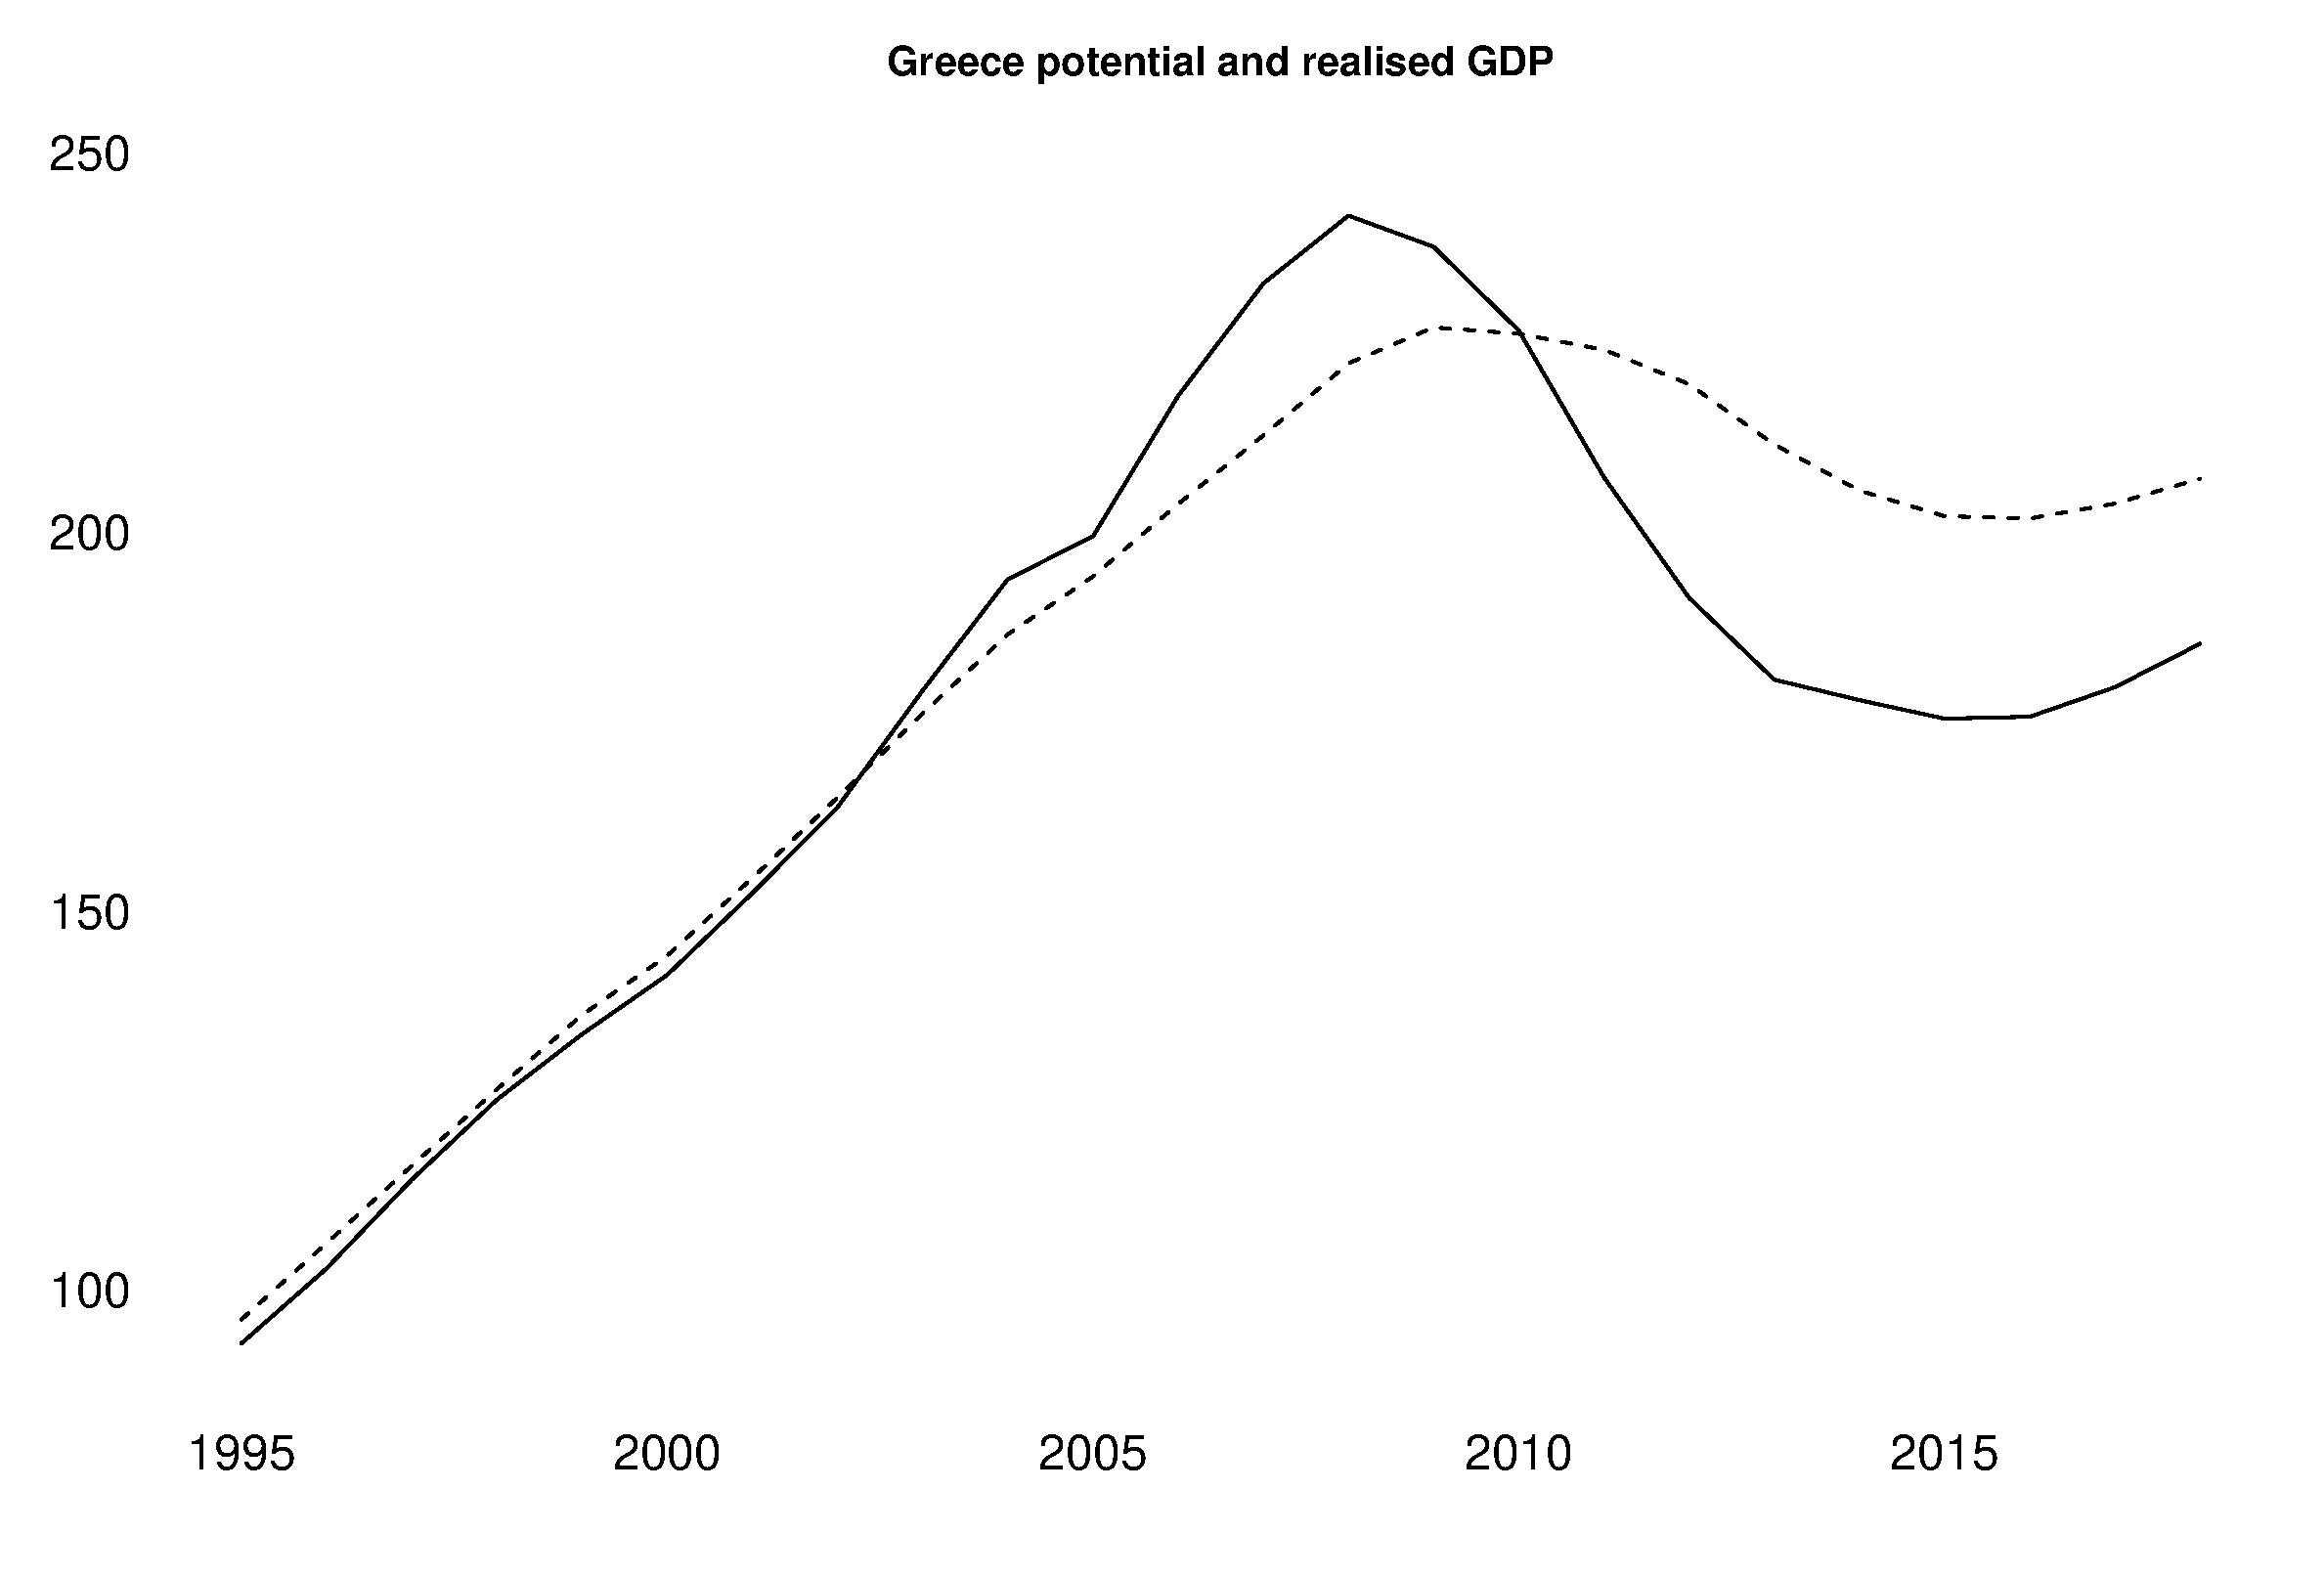
\includegraphics[scale=.3]{greece5.eps}
  \end{figure}
\end{frame}
%--------------------------------------


%--------------------------------------
\begin{frame}
  \textbf{ECB response} to eurocrisis\\
   ECB's preferred course of action: do nothing
   \begin{itemize}
      \item Governments should clear up mess
      \item Recall ECB independence: in order to limit government interference in its policy
    \end{itemize} 
    \medskip
    Unatainable as crisis progressed    
    \begin{itemize}
      \item Main fear: contagion of crisis from periphery to central economies
      \item Serious risk: Italy owed France about 20\% of French GDP
    \end{itemize}
\end{frame}
%--------------------------------------

%--------------------------------------
\begin{frame}
  \textbf{Lisbon treaty} article 123
  \scalebox{.7}{
  \begin{quote}
    1. Overdraft facilities or any other type of credit facility with the European Central Bank or with the central banks of the Member States (hereinafter referred to as ‘national central banks’) in favour of Union institutions, bodies, offices or agencies, central governments, regional, local or other public authorities, other bodies governed by public law, or public undertakings of Member States shall be prohibited, as shall the purchase directly from them by the European Central Bank or national central banks of debt instruments.

    2. Paragraph 1 shall not apply to publicly owned credit institutions which, in the context of the supply of reserves by central banks, shall be given the same treatment by national central banks and the European Central Bank as private credit institutions.
    \end{quote}}
\end{frame}
%--------------------------------------


%--------------------------------------
\begin{frame}
  ECB took two measures
  \begin{enumerate}
    \item Standard
  \begin{itemize}
    \item Downward adjustment of key interest rates
    \item Taken due to the macroeconomic circumstances and the risk for price stability
    \item Short-term interest rates are close to zero at the moment
  \end{itemize}
  \medskip
  \item Non-Standard
  \begin{itemize}
    \item Includes fixed rate lending, providing longer maturity liquidity, expanding set of assets that can serve as collateral
    \item Taken because banking system wasn't functioning properly: ECB needs proper transmission mechanisms for monetary policy    
  \end{itemize}
  \end{enumerate}
\end{frame}
%--------------------------------------


%--------------------------------------
\begin{frame}
  ECB also took number of unconventional steps
  \begin{enumerate}    
    \item Securities Market Program (SMP)
    \item Long Term Refinancing Operations (LTRO)
    \item Outright Money Transactions (OMT) 
  \end{enumerate}
\end{frame}
%--------------------------------------

%--------------------------------------
\begin{frame}
  \textbf{Securities Market Program}
  \begin{itemize}
    \item Purchasing government and private debt, from countries facing problems
    \item Similar to QE, main difference is that ECB keeps the books balanced; offsetting the purchases by offering the banks interest-bearing deposits
  \end{itemize}
  \medskip
  \textbf{Long Term Refinancing Operations}
  \begin{itemize}
    \item ECB committed to refinancing operations for multiple years, rather than couple of months which is common    
    \item ECB serves as lender of first resort to troubled banks, these banks could then help struggling governments by purchasing debt    
  \end{itemize}
  \medskip  
  \textbf{Outright Money Transactions}
  \begin{itemize}
    \item Under certain circumstances a state could request the ECB to buy bonds     
    \item OMTs haven't been used yet as none of the candidate countries met the criteria
  \end{itemize}
\end{frame}
%--------------------------------------

%--------------------------------------
\begin{frame}
  \begin{figure}
    \includegraphics[scale=.4]{ecb.eps}
  \end{figure}
\end{frame}
%--------------------------------------

%--------------------------------------
\begin{frame} 
  EU economic and monetary integration is all about convergence
  \begin{itemize}
    \item Raising living standards
    \item Reducing gap between Western Europe and the rest
  \end{itemize}
  \medskip
  Went well for long time; early 2000s seemed promising
  \begin{itemize}
    \item Crisis put serious dent in progress: setting countries back a decade
    \item Led to new divergence
  \end{itemize}
\end{frame}
%--------------------------------------

%--------------------------------------
\begin{frame}
  \begin{figure}
    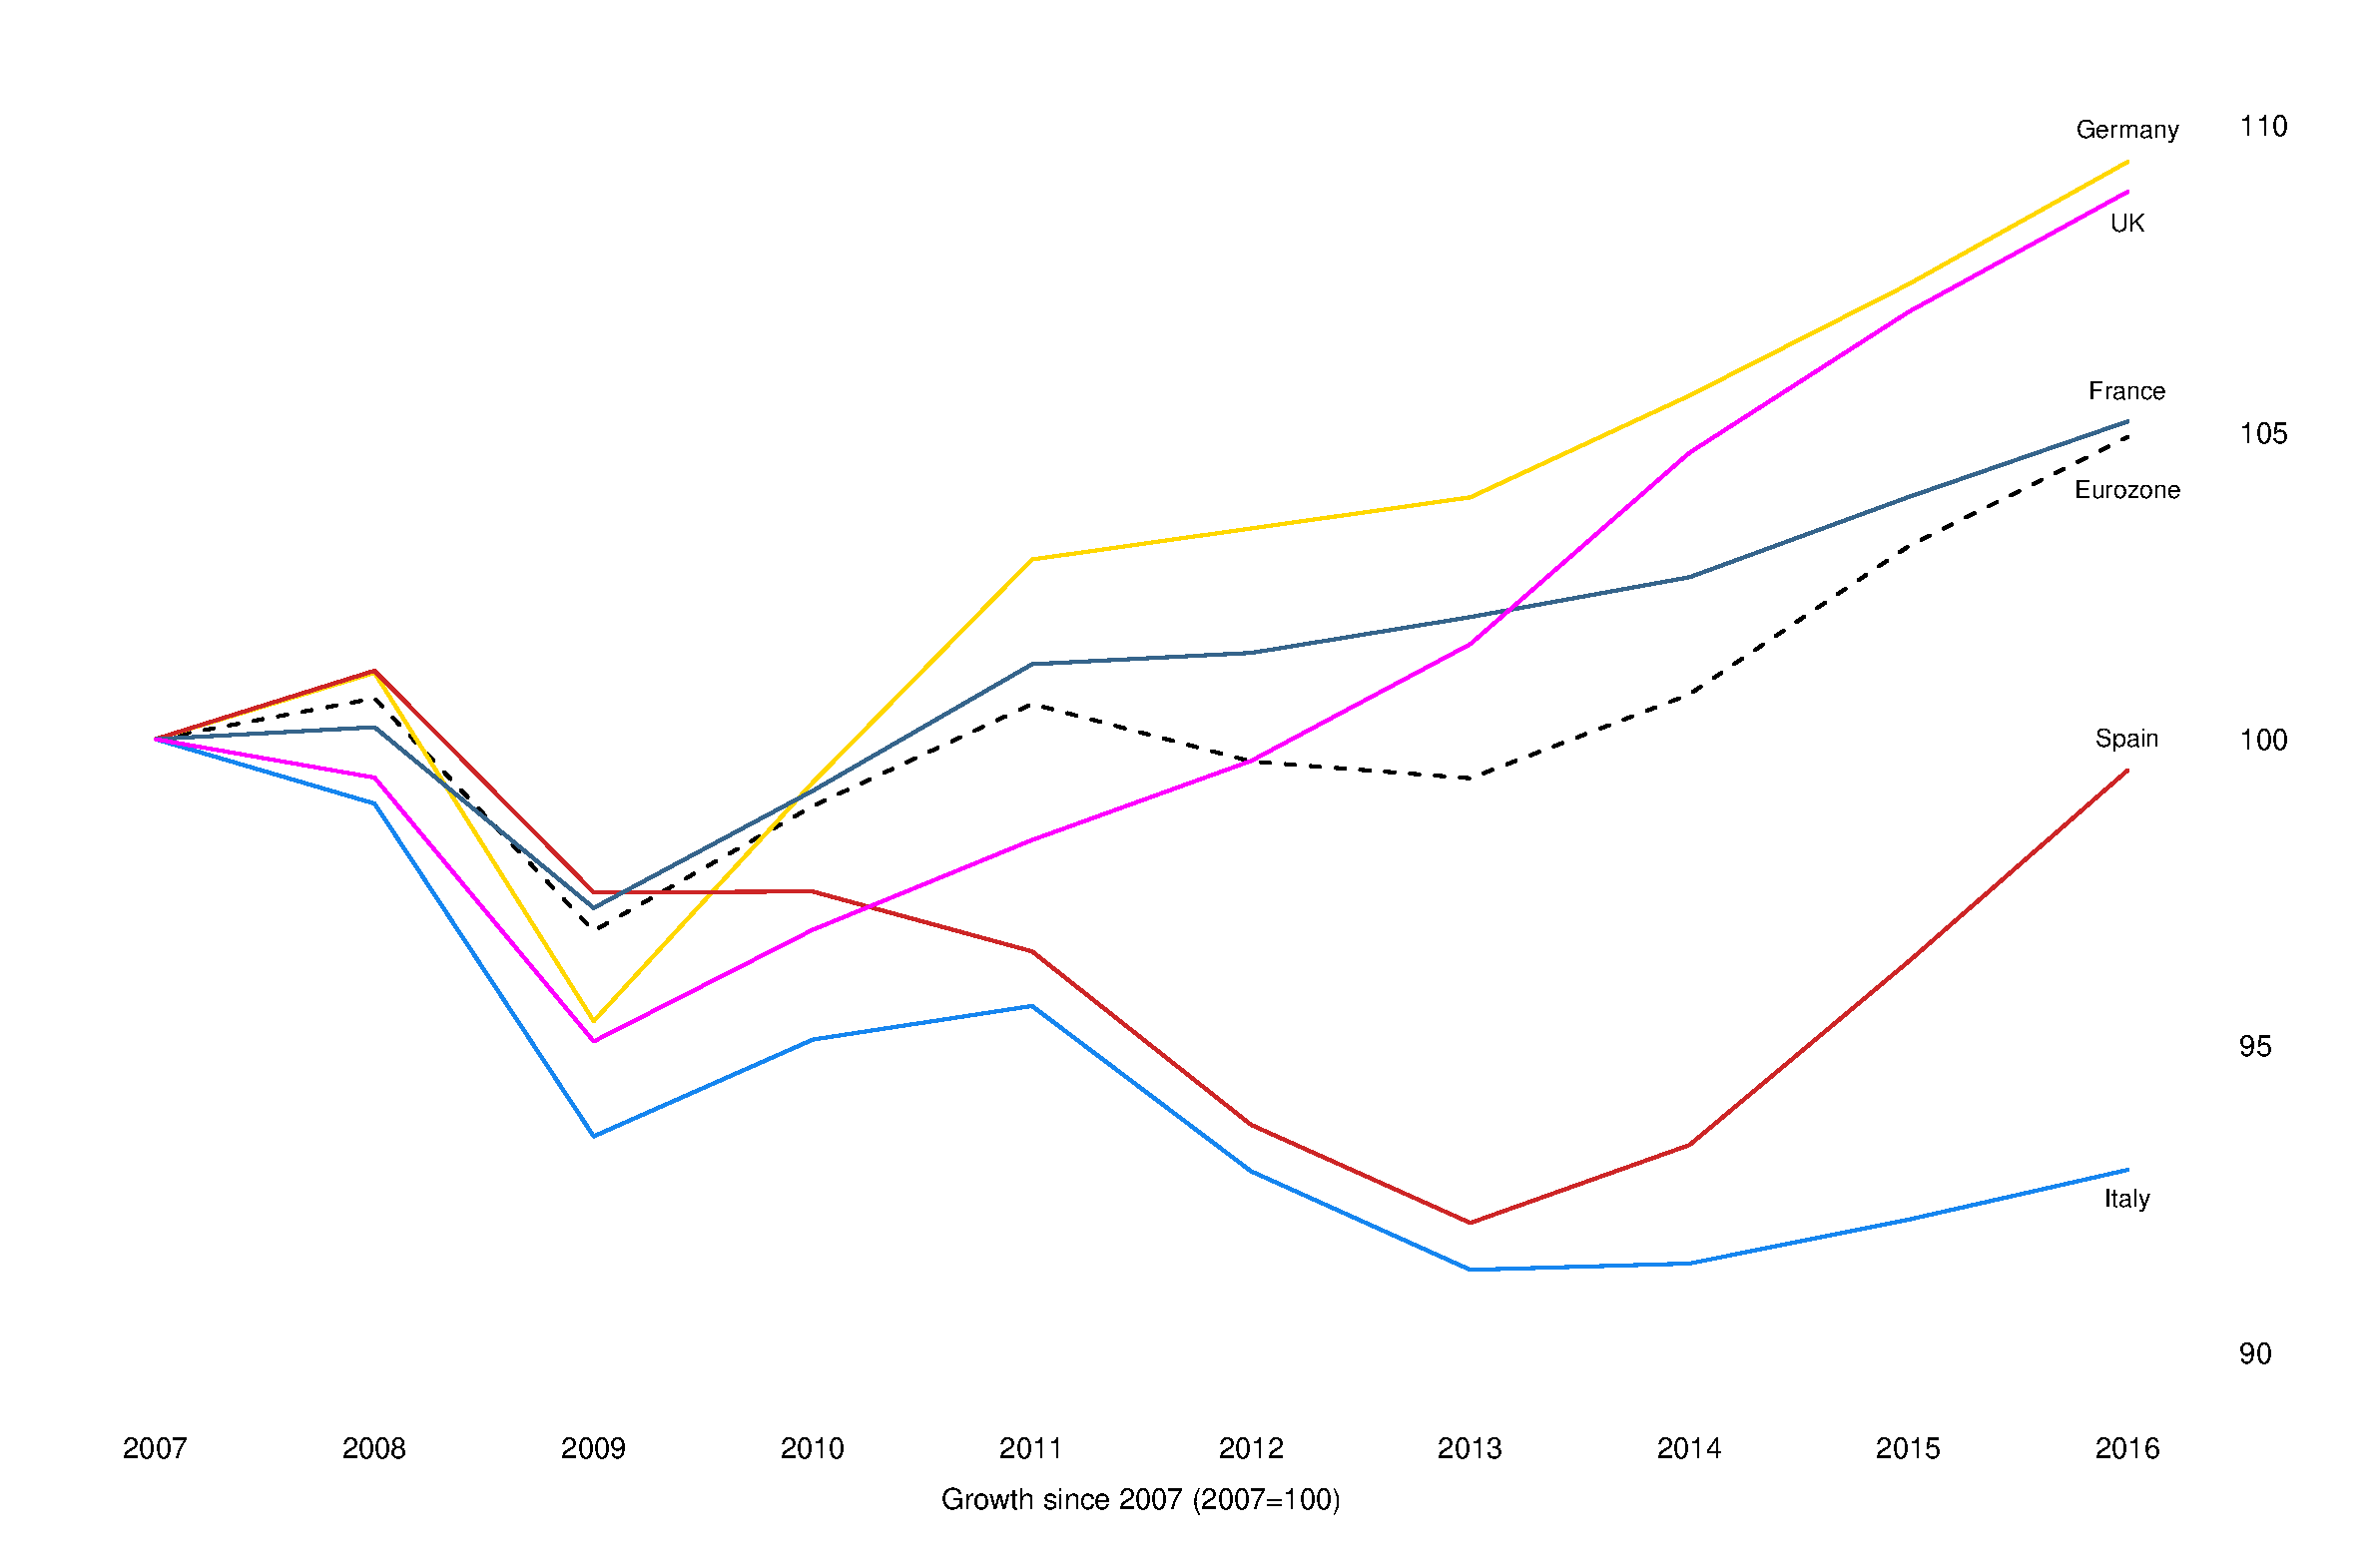
\includegraphics[scale=.3]{economic_growth.eps}
  \end{figure}
\end{frame}
%--------------------------------------

%--------------------------------------
\begin{frame}
  \begin{figure}
    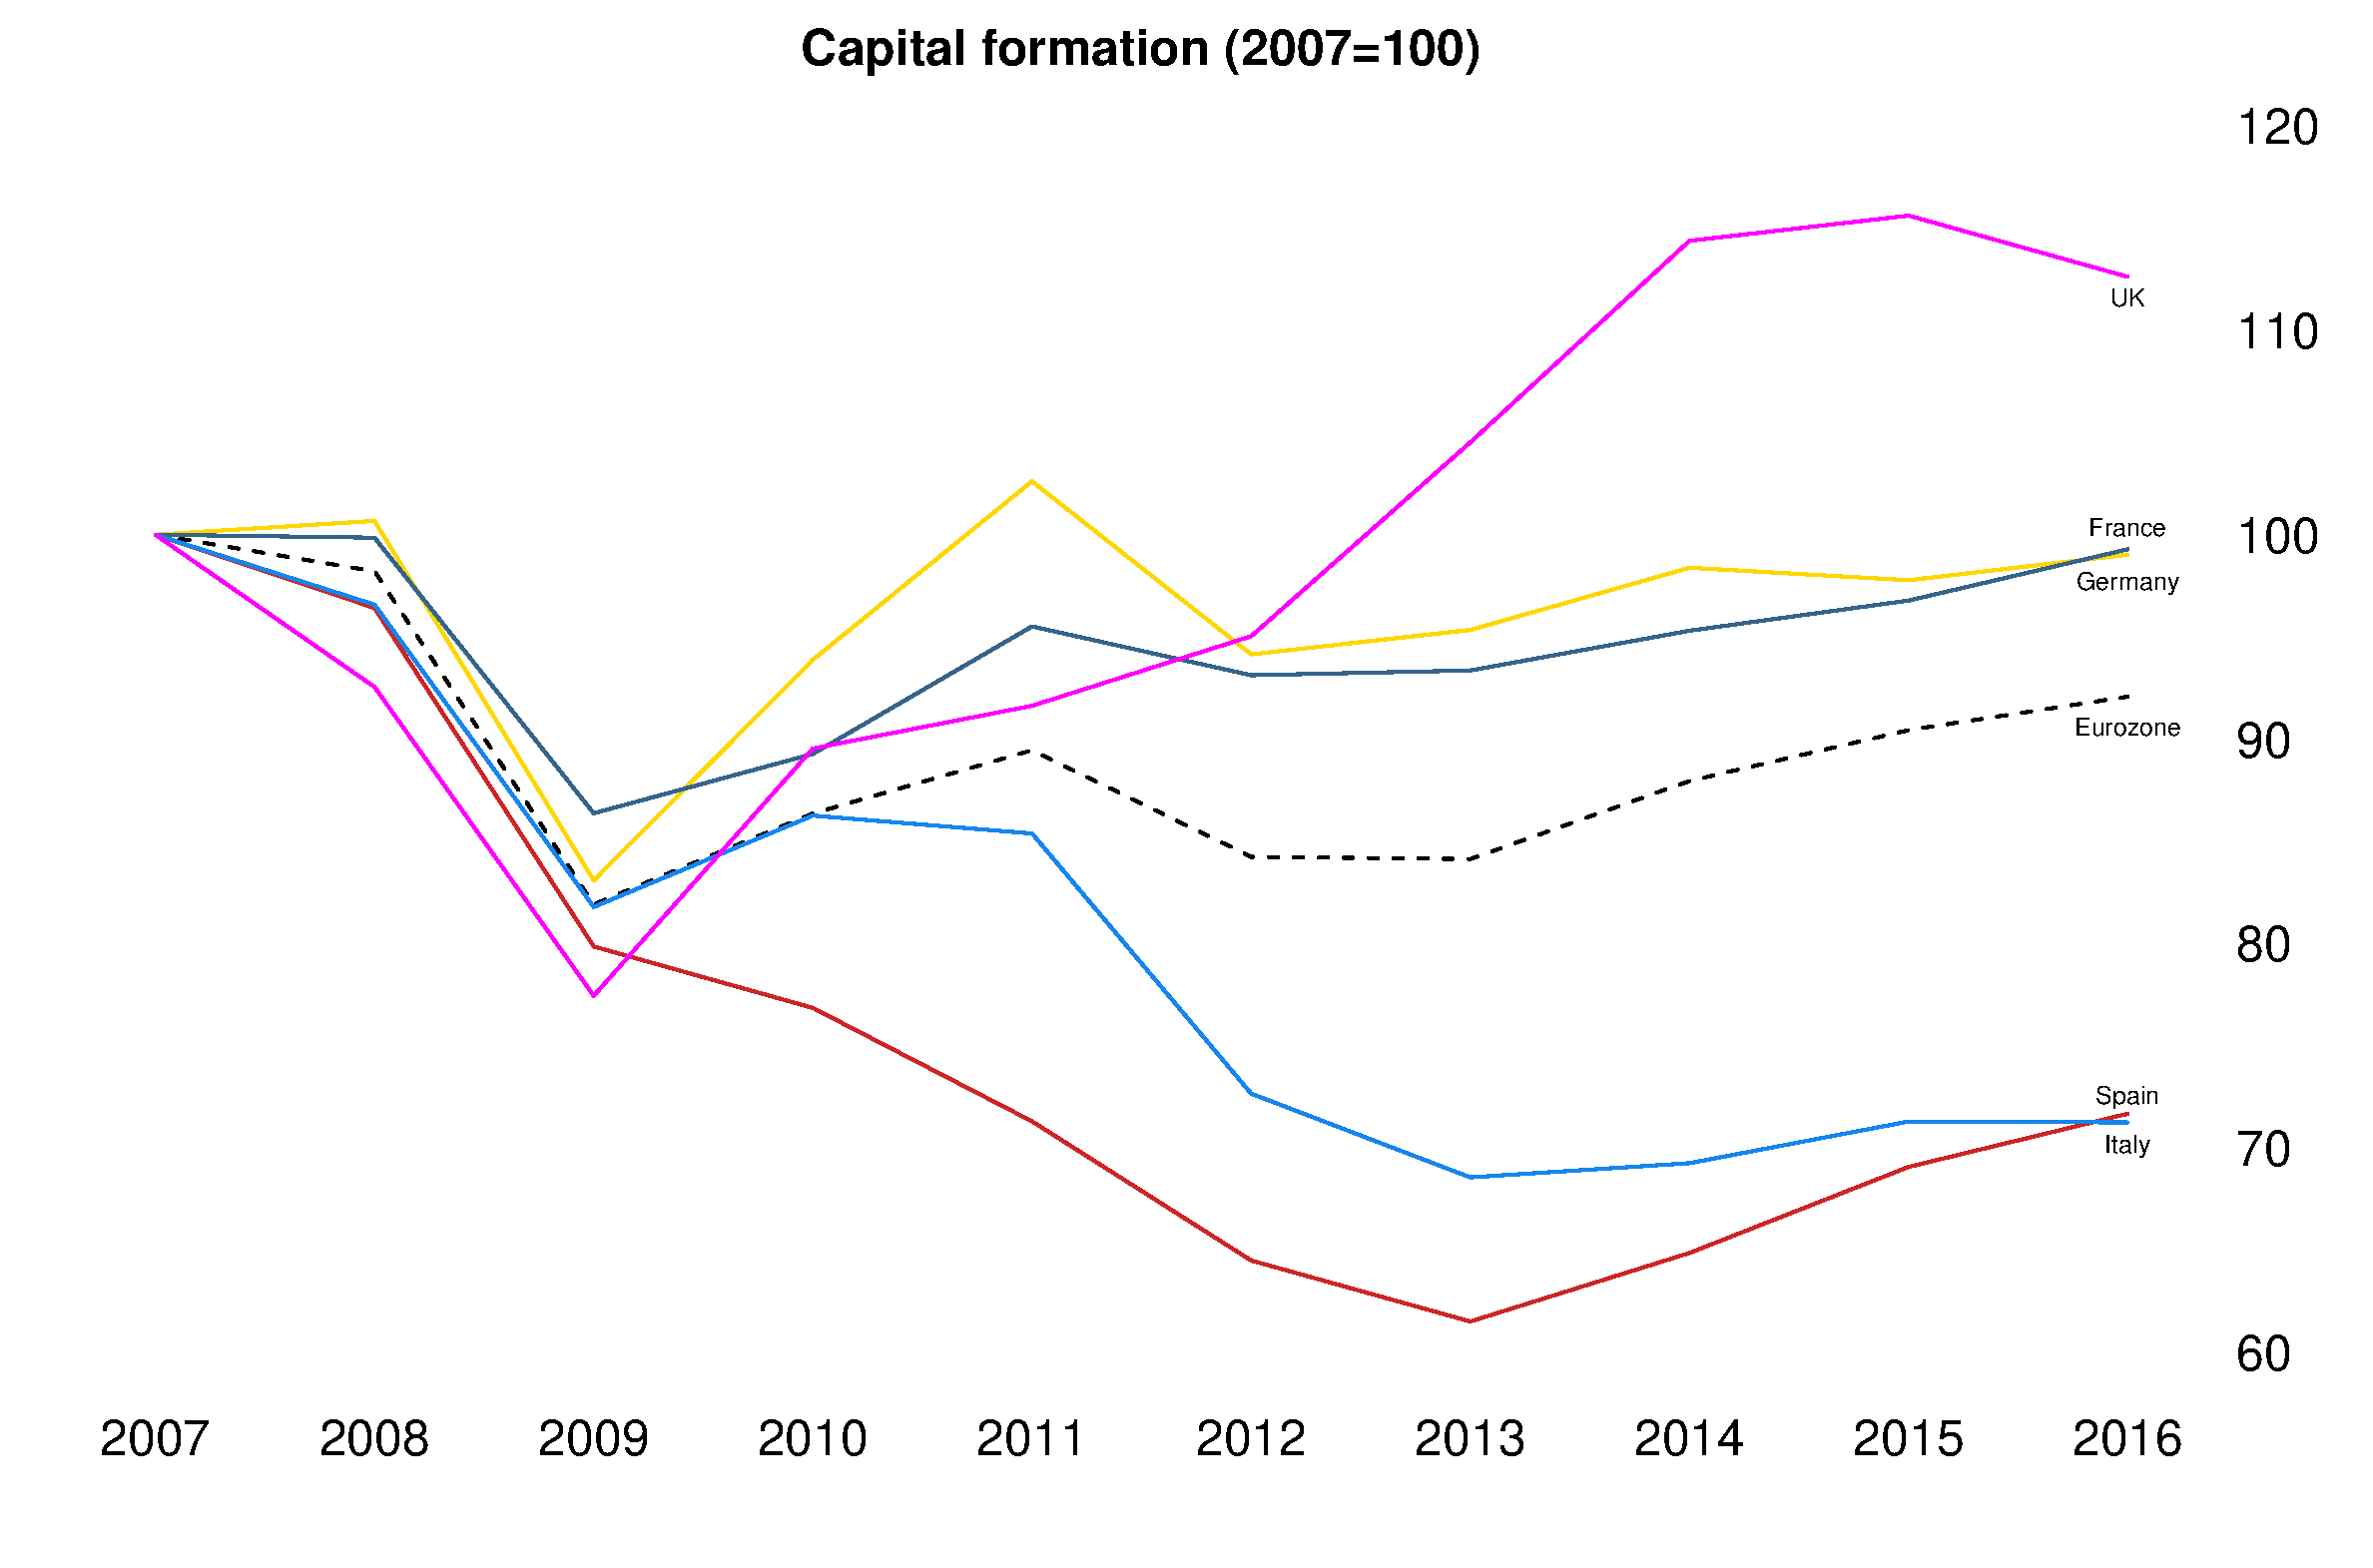
\includegraphics[scale=.3]{capital_formation.eps}
  \end{figure}
\end{frame}
%--------------------------------------

%--------------------------------------
\begin{frame}
  \begin{figure}
    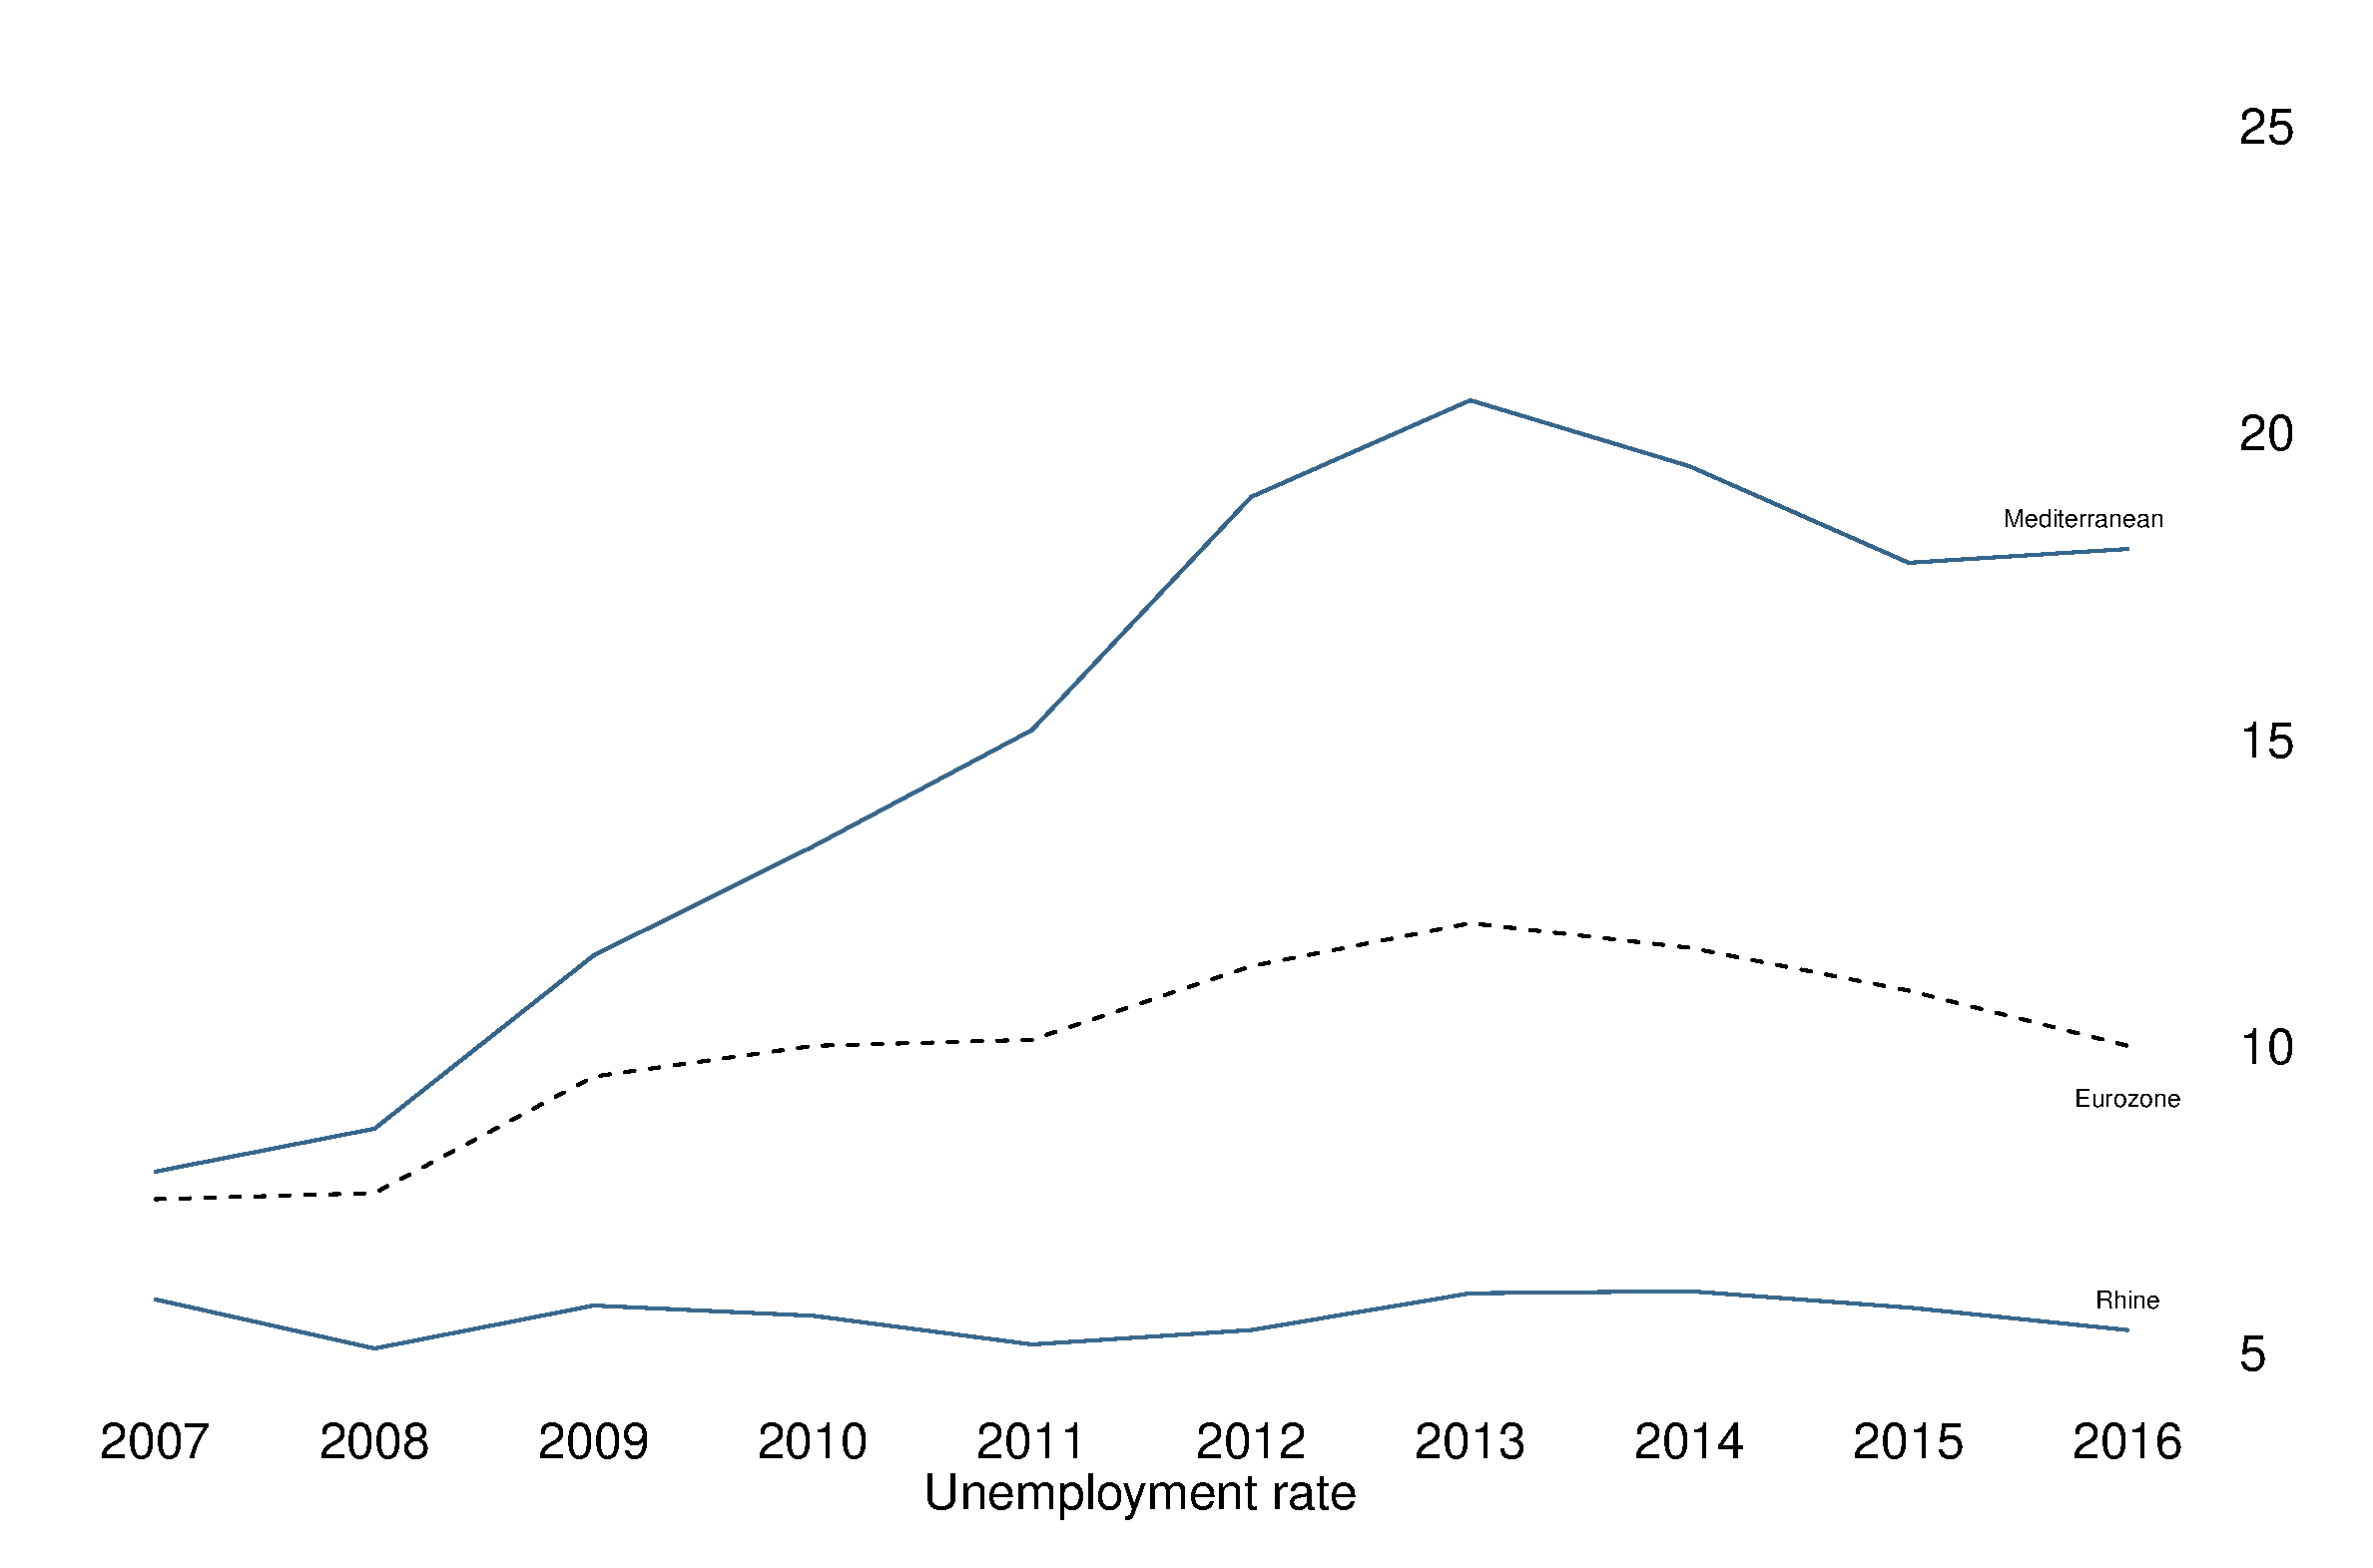
\includegraphics[scale=.3]{unemployment.eps}
  \end{figure}
\end{frame}
%--------------------------------------

%--------------------------------------
\begin{frame}
  \begin{figure}
    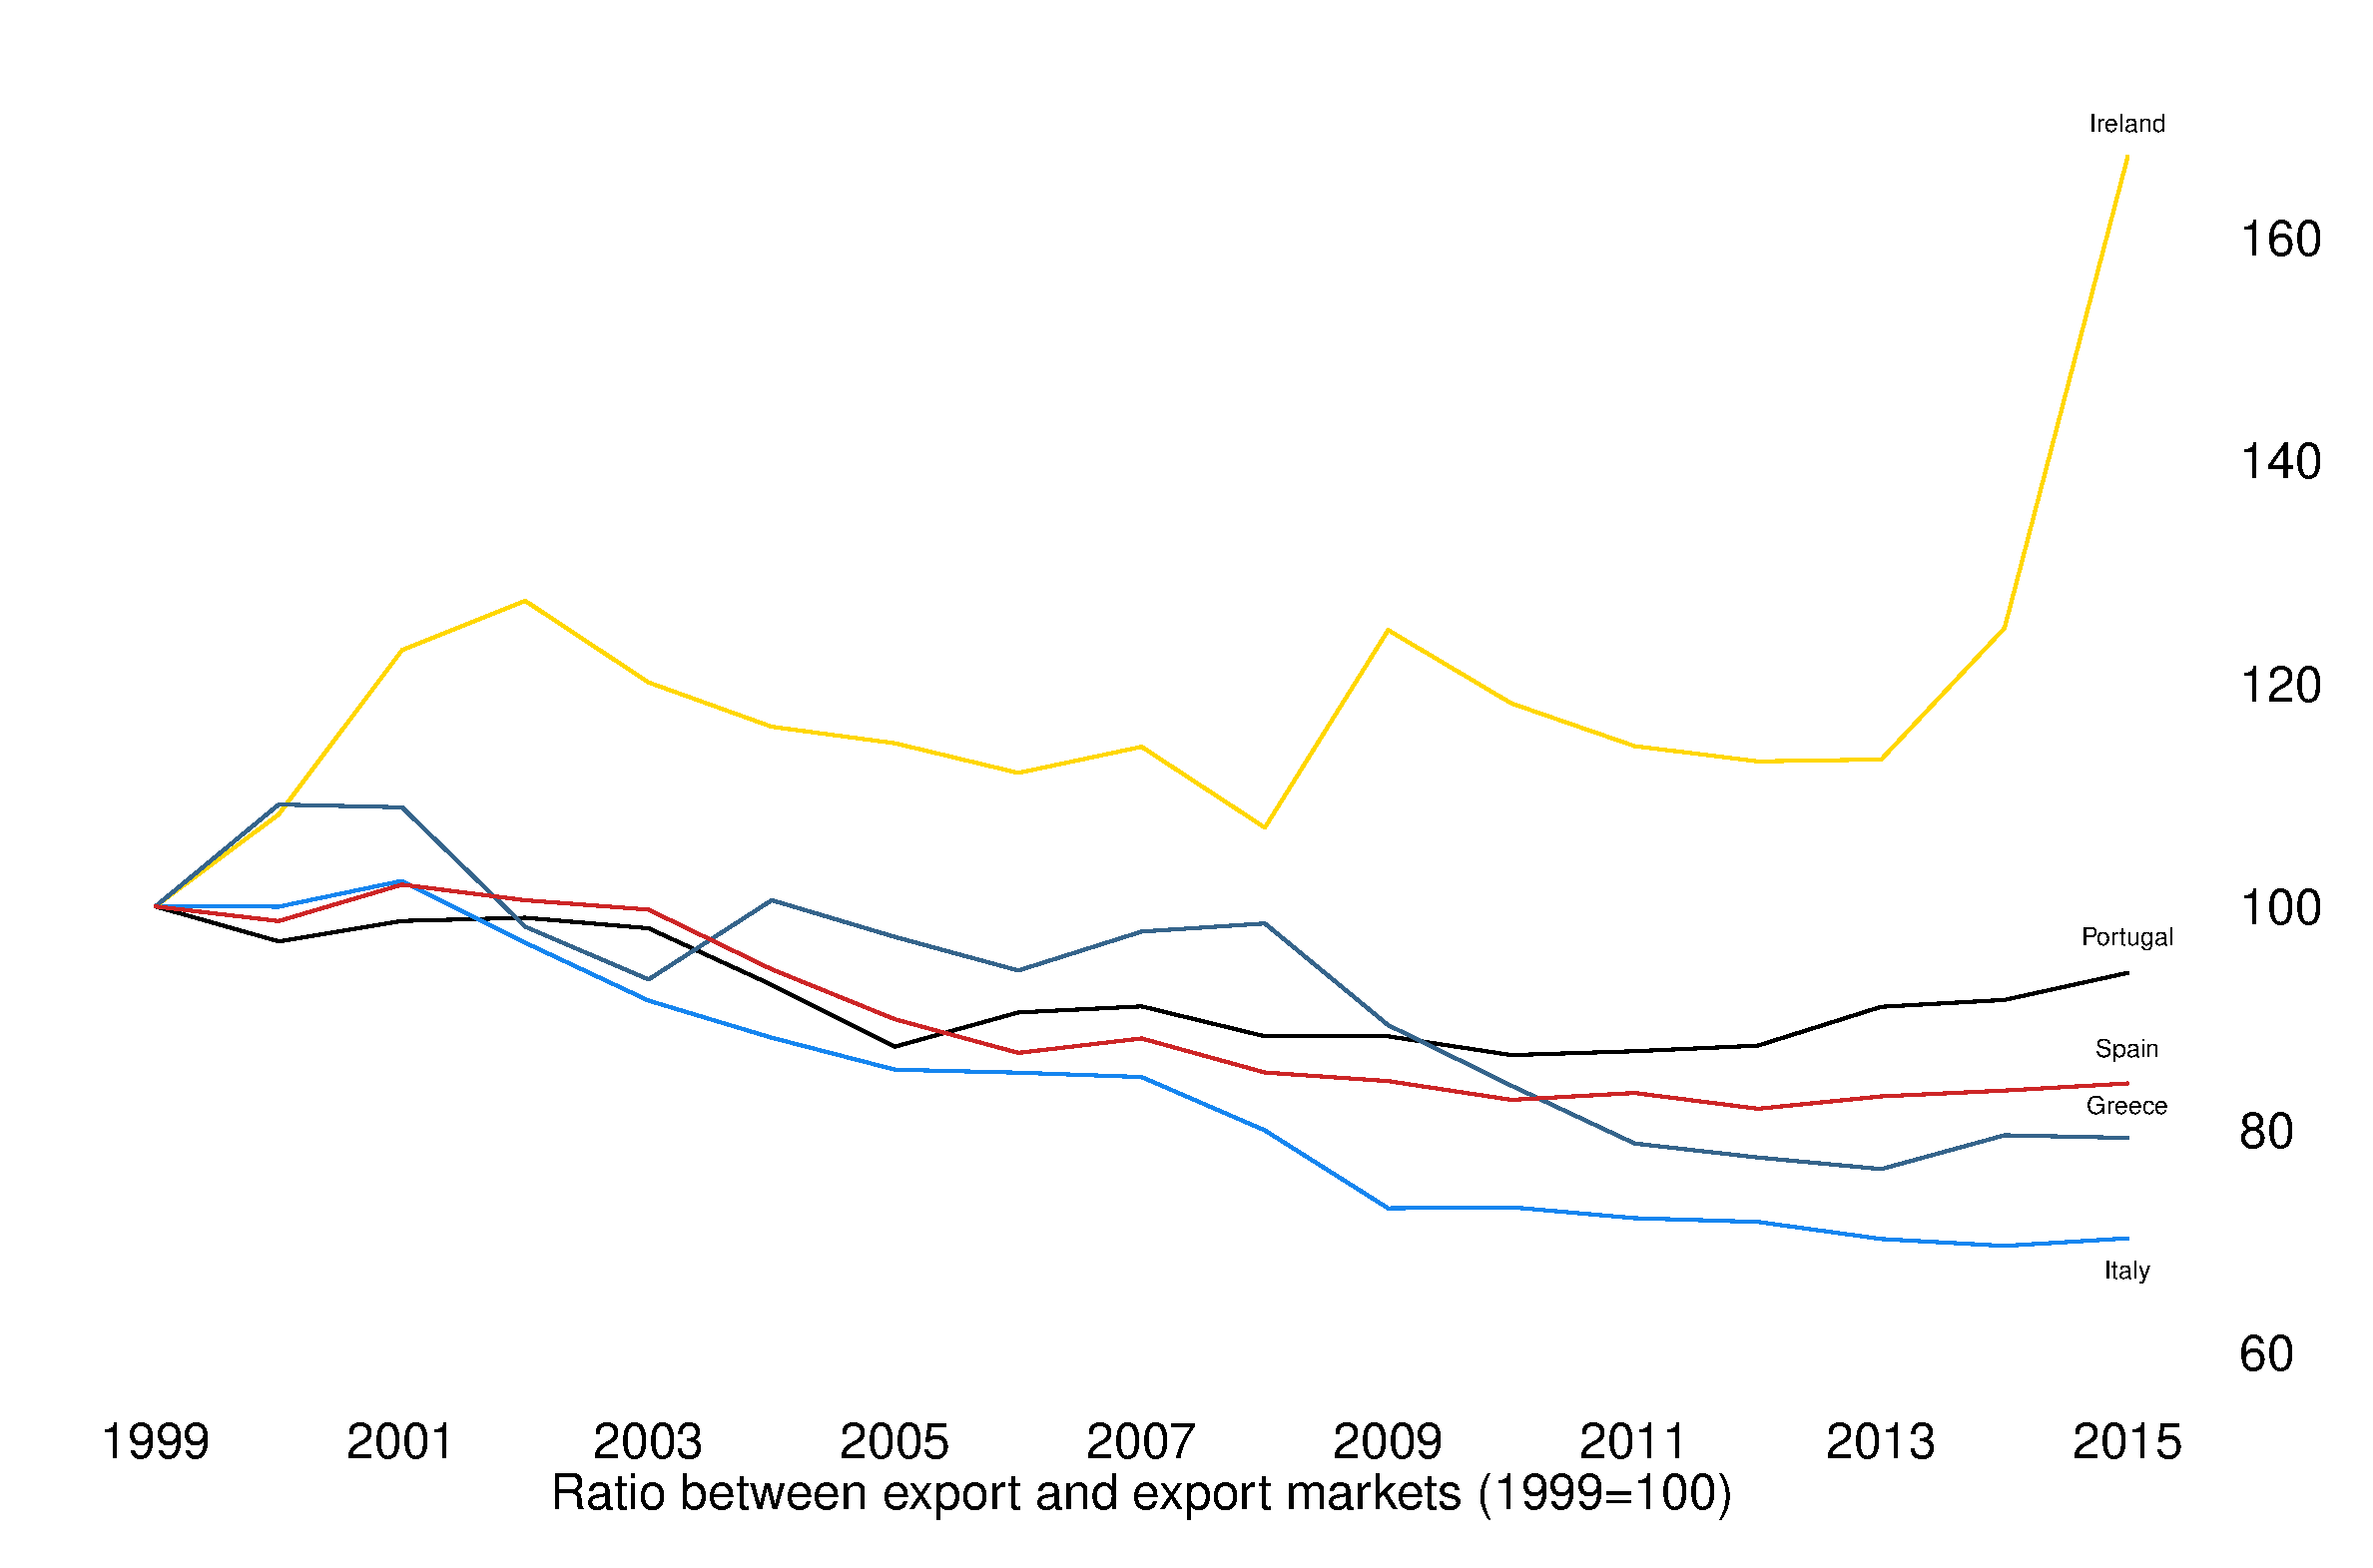
\includegraphics[scale=.3]{pigs_exports.eps}
  \end{figure}
\end{frame}
%--------------------------------------

%--------------------------------------
\begin{frame}
  \begin{figure}
    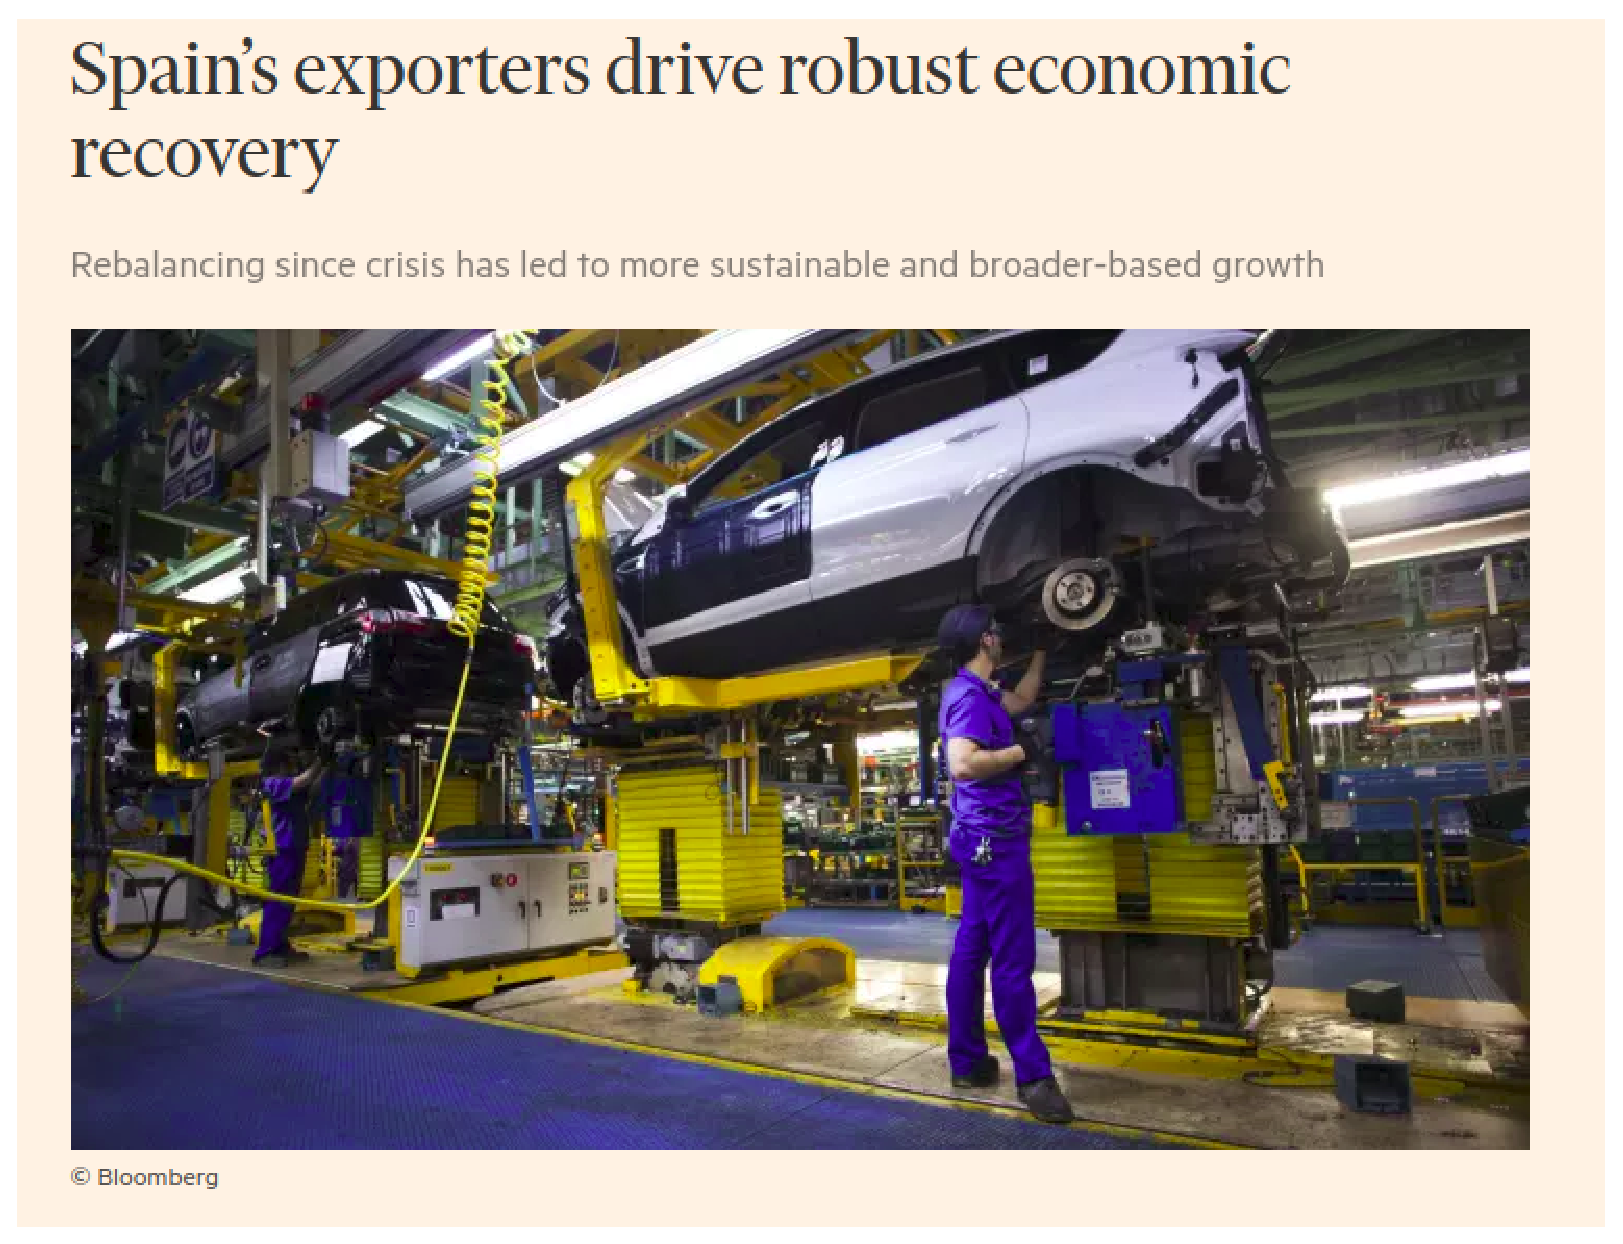
\includegraphics[scale=.4]{spain2.eps}
  \end{figure}
\end{frame}
%--------------------------------------

%--------------------------------------
\end{document}

